 % -*- Mode:TeX -*-

%% IMPORTANT: The official thesis specifications are available at:
%%            http://libraries.mit.edu/archives/thesis-specs/
%%
%%            Please verify your thesis' formatting and copyright
%%            assignment before submission.  If you notice any
%%            discrepancies between these templates and the 
%%            MIT Libraries' specs, please let us know
%%            by e-mailing thesis@mit.edu

%% The documentclass options along with the pagestyle can be used to generate
%% a technical report, a draft copy, or a regular thesis.  You may need to
%% re-specify the pagestyle after you \include  cover.tex.  For more
%% information, see the first few lines of mitthesis.cls. 

%\documentclass[12pt,vi,twoside]{mitthesis}
%%
%%  If you want your thesis copyright to you instead of MIT, use the
%%  ``vi'' option, as above.
%%
%\documentclass[12pt,twoside,leftblank]{mitthesis}
%%
%% If you want blank pages before new chapters to be labelled ``This
%% Page Intentionally Left Blank'', use the ``leftblank'' option, as
%% above. 

\documentclass[12pt,twoside,fleqn]{mitthesis}
\usepackage{graphicx,xcolor}
\usepackage{booktabs}
\usepackage[font={small}]{caption}
\usepackage[labelfont=bf]{caption}
\captionsetup[algorithm]{font=small}
\usepackage{notoccite}
\usepackage{lgrind}
\pagestyle{plain}
\usepackage{url}
\usepackage{algorithm}
\usepackage[noend]{algpseudocode}
\usepackage[english]{babel}
\usepackage{amssymb}
\usepackage[utf8]{inputenc}
\usepackage{enumerate}
\usepackage{hyperref}
\usepackage{amsmath}
\hypersetup{colorlinks=true, linkcolor={black}, citecolor={blue}, urlcolor={magenta}}
\usepackage{emptypage}
\usepackage{eso-pic}


%% This bit allows you to either specify only the files which you wish to
%% process, or `all' to process all files which you \include.
%% Krishna Sethuraman (1990).
%
%\typein [\files]{Enter file names to process, (chap1,chap2 ...), or `all' to process all files:}
%\def\all{all}
%\ifx\files\all \typeout{Including all files.} \else \typeout{Including only \files.} \includeonly{\files} \fi

\begin{document}
% -*-latex-*-
% 
% For questions, comments, concerns or complaints:
% thesis@mit.edu
% 
%
% $Log: cover.tex,v $
% Revision 1.8  2008/05/13 15:02:15  jdreed
% Degree month is June, not May.  Added note about prevdegrees.
% Arthur Smith's title updated
%
% Revision 1.7  2001/02/08 18:53:16  boojum
% changed some \newpages to \cleardoublepages
%
% Revision 1.6  1999/10/21 14:49:31  boojum
% changed comment referring to documentstyle
%
% Revision 1.5  1999/10/21 14:39:04  boojum
% *** empty log message ***
%
% Revision 1.4  1997/04/18  17:54:10  othomas
% added page numbers on abstract and cover, and made 1 abstract
% page the default rather than 2.  (anne hunter tells me this
% is the new institute standard.)
%
% Revision 1.4  1997/04/18  17:54:10  othomas
% added page numbers on abstract and cover, and made 1 abstract
% page the default rather than 2.  (anne hunter tells me this
% is the new institute standard.)
%
% Revision 1.3  93/05/17  17:06:29  starflt
% Added acknowledgements section (suggested by tompalka)
% 
% Revision 1.2  92/04/22  13:13:13  epeisach
% Fixes for 1991 course 6 requirements
% Phrase "and to grant others the right to do so" has been added to 
% permission clause
% Second copy of abstract is not counted as separate pages so numbering works
% out
% 
% Revision 1.1  92/04/22  13:08:20  epeisach

% NOTE:
% These templates make an effort to conform to the MIT Thesis specifications,
% however the specifications can change.  We recommend that you verify the
% layout of your title page with your thesis advisor and/or the MIT 
% Libraries before printing your final copy.
\title{Automatic calibration of an urban microclimate model under uncertainty \vspace{12pt}}

\author{Jiachen Mao}
\prevdegrees{B.Eng., Tongji University (2015) \vspace{12pt}}
\department{Department of Architecture}

\degree{\vspace{12pt} Master of Science in Building Technology \vspace{12pt}}

% If you wish to list your previous degrees on the cover page, use the 
% previous degrees command:
%       \prevdegrees{A.A., Harvard University (1985)}
% You can use the \\ command to list multiple previous degrees
%       \prevdegrees{B.S., University of California (1978) \\
%                    S.M., Massachusetts Institute of Technology (1981)}

% If the thesis is for two degrees simultaneously, list them both
% separated by \and like this:
% \degree{Doctor of Philosophy \and Master of Science}

% As of the 2007-08 academic year, valid degree months are September, 
% February, or June.  The default is June.
\degreemonth{September}
\degreeyear{2018}
\thesisdate{August 10, 2018}

%% By default, the thesis will be copyrighted to MIT.  If you need to copyright
%% the thesis to yourself, just specify the `vi' documentclass option.  If for
%% some reason you want to exactly specify the copyright notice text, you can
%% use the \copyrightnoticetext command.  
%\copyrightnoticetext{\copyright IBM, 1990.  Do not open till Xmas.}

% If there is more than one supervisor, use the \supervisor command
% once for each.
\supervisor{Leslie K. Norford}{George Macomber (1948) Professor in Construction Management}

% This is the department committee chairman, not the thesis committee
% chairman.  You should replace this with your Department's Committee
% Chairman.
\chairman{Sheila Kennedy}{Professor of Architecture\\Chairman, Department Committee on Graduate Students}

% Make the titlepage based on the above information.  If you need
% something special and can't use the standard form, you can specify
% the exact text of the titlepage yourself.  Put it in a titlepage
% environment and leave blank lines where you want vertical space.
% The spaces will be adjusted to fill the entire page.  The dotted
% lines for the signatures are made with the \signature command.
\maketitle

% The abstractpage environment sets up everything on the page except
% the text itself.  The title and other header material are put at the
% top of the page, and the supervisors are listed at the bottom.  A
% new page is begun both before and after.  Of course, an abstract may
% be more than one page itself.  If you need more control over the
% format of the page, you can use the abstract environment, which puts
% the word "Abstract" at the beginning and single spaces its text.

%% You can either \input (*not* \include) your abstract file, or you can put
%% the text of the abstract directly between the \begin{abstractpage} and
%% \end{abstractpage} commands.

% First copy: start a new page, and save the page number.
\cleardoublepage
% Uncomment the next line if you do NOT want a page number on your
% abstract and acknowledgments pages.
% \pagestyle{empty}
\setcounter{savepage}{\thepage}
\begin{abstractpage}
% $Log: abstract.tex,v $
% Revision 1.1  93/05/14  14:56:25  starflt
% Initial revision
% 
% Revision 1.1  90/05/04  10:41:01  lwvanels
% Initial revision
% 
%
%% The text of your abstract and nothing else (other than comments) goes here.
%% It will be single-spaced and the rest of the text that is supposed to go on
%% the abstract page will be generated by the abstractpage environment.  This
%% file should be \input (not \include 'd) from cover.tex.
Simulation models play an important role in the design, analysis, and optimization of modern energy and environmental systems at building or urban scale. However, due to the extreme complexity of built environments and the sheer number of interacting parameters, it is difficult to obtain an accurate representation of real-world systems. Thus, model calibration and uncertainty analysis hold a particular interest, and it is necessary to evaluate to what degree simulation models are imperfect before implementing them during the decision-making process. In contrast to the extensive literature on the calibration of building performance models, little has been reported on how to automatically calibrate physics-based urban microclimate models. 

This thesis illustrates a general methodology for automatic model calibration and, for the first time, applies it to an urban microclimate system. The study builds upon the previously reported and updated Urban Weather Generator (UWG) to present a deep look into an existing urban district area in downtown Abu Dhabi (UAE) during 2017. Based on 30 candidate inputs covering the meteorological factors, urban characteristics, vegetation variables, and building systems, we performed global sensitivity analysis, Monte Carlo filtering, and optimization-aided calibration on the UWG model. In particular, an online hyper-heuristic evolutionary algorithm (EA) is proposed and developed to accelerate the calibration process. The UWG is a fairly robust simulator to approximate the urban thermal behavior for different seasons. The validation results show that, in single-objective optimization, the online hyper-heuristics can robustly help EA produce quality solutions with smaller uncertainties at much less computational cost. Finally, the resulting calibrated solutions are able to capture weekly-average and hourly diurnal profiles of the urban outdoor air temperature similar to the measurements for certain periods of the year.

\end{abstractpage}

% Additional copy: start a new page, and reset the page number.  This way,
% the second copy of the abstract is not counted as separate pages.
% Uncomment the next 6 lines if you need two copies of the abstract
% page.
% \setcounter{page}{\thesavepage}
% \begin{abstractpage}
% % $Log: abstract.tex,v $
% Revision 1.1  93/05/14  14:56:25  starflt
% Initial revision
% 
% Revision 1.1  90/05/04  10:41:01  lwvanels
% Initial revision
% 
%
%% The text of your abstract and nothing else (other than comments) goes here.
%% It will be single-spaced and the rest of the text that is supposed to go on
%% the abstract page will be generated by the abstractpage environment.  This
%% file should be \input (not \include 'd) from cover.tex.
Simulation models play an important role in the design, analysis, and optimization of modern energy and environmental systems at building or urban scale. However, due to the extreme complexity of built environments and the sheer number of interacting parameters, it is difficult to obtain an accurate representation of real-world systems. Thus, model calibration and uncertainty analysis hold a particular interest, and it is necessary to evaluate to what degree simulation models are imperfect before implementing them during the decision-making process. In contrast to the extensive literature on the calibration of building performance models, little has been reported on how to automatically calibrate physics-based urban microclimate models. 

This thesis illustrates a general methodology for automatic model calibration and, for the first time, applies it to an urban microclimate system. The study builds upon the previously reported and updated Urban Weather Generator (UWG) to present a deep look into an existing urban district area in downtown Abu Dhabi (UAE) during 2017. Based on 30 candidate inputs covering the meteorological factors, urban characteristics, vegetation variables, and building systems, we performed global sensitivity analysis, Monte Carlo filtering, and optimization-aided calibration on the UWG model. In particular, an online hyper-heuristic evolutionary algorithm (EA) is proposed and developed to accelerate the calibration process. The UWG is a fairly robust simulator to approximate the urban thermal behavior for different seasons. The validation results show that, in single-objective optimization, the online hyper-heuristics can robustly help EA produce quality solutions with smaller uncertainties at much less computational cost. Finally, the resulting calibrated solutions are able to capture weekly-average and hourly diurnal profiles of the urban outdoor air temperature similar to the measurements for certain periods of the year.

% \end{abstractpage}

\cleardoublepage

\chapter*{Acknowledgments}

Summary is a skill that may take years to master, a period of time which perhaps I have not fully experienced, thus making my gratitude to those, who have managed to help me relieve my stress and make MIT my beloved home over these two years, with short statements a formidable challenge that goes beyond any of my reasonable articulation. But if there is one thing that I have learned along with the experience that formed this work, it is to challenge the convention, extend the boundary, and believe in yourself.

All my education and research at MIT over these two years have taught me that getting the ultimate correct answer toward any question may never be possible, but it is always possible to answer it to your best knowledge and effort. That answer, I believe, is already useful for many things and people in this world. Here, I shall make an attempt to answer the question again and do what I think to be not shy of impossible -- express my appreciation in a summary.

First and foremost, to my dear advisor, Professor \textit{Leslie K. Norford}, who has absolutely exceeded my expectations, not just in the academic work, but also in his virtue on my journey toward wisdom, pragmatism, and philosophy. In various ways, Les is truly one of the very best role models I could wish to have in my life. While I may be striving to solve problems in the future beyond his wing, I will always look up to him with my highest respect, rectitude, and honor.

There is another person who has surpassed my reasonable notion. I would like to deliver my sincere gratitude to my dear friend, Professor \textit{Afshin Afshari}, who devoted his effort and time to introduce me his splendid research and remotely offer me any help, although we have never met in person. With his exceptional charm, Afshin has always been there for support and advice, which I shall never forget.

In addition, \textit{Yangyang Fu} deserves to be recognized and appreciated. Suffice to say, Yangyang is the one whom at the start of my research during college I thought to be an ordinary labmate but turned out to be a true friend who has supported me any time when I need. He has been a critical part leading to the completion of this thesis, consequently contributing to a lot of my nostalgic memories over time.

I surely would not be honest if I do not admit that there were many others who have provided help for this work. Namely, I would like to thank Professor \textit{Peter R. Armstrong} for supplying the very important data and his insightful comments on my thesis. I would also want to express my great thank-you to Drs. \textit{Peter J. Kempthorne} and \textit{Victor-Emmanual Brunel} for their advice on the uncertainty/sensitivity analysis, to Professors \textit{Dimitris J. Bertsimas} and \textit{Patrick Jaillet} for their advice on the optimization algorithm, and to \textit{Qinzi Luo} for the discussions on the HVAC system.

Finally, I would like to gratefully acknowledge that this research was carried out at the MIT Building Technology Lab with sponsorship supported by the MIT/Masdar Institute Collaborative Program (Ref. No. 02/MI/MIT/CP/11/07633/GEN/G/00), the Leon Hyzen Fellowship, and the George Macomber Chair Scholarship from 2016 to 2018. The views and opinions expressed in this thesis are those of the author and hereby do not necessarily reflect the official policy or position of any agency. Possible errors in the thesis indicate the limitations of the author, who nevertheless hopes the underlying insights could benefit others.


\cleardoublepage

\vspace*{2.5in}
\hspace*{\fill}
\textit{To my dear parents.}
%\hspace*{\fill}
\vspace*{\fill}


%%%%%%%%%%%%%%%%%%%%%%%%%%%%%%%%%%%%%%%%%%%%%%%%%%%%%%%%%%%%%%%%%%%%%%
% -*-latex-*-

% Some departments (e.g. 5) require an additional signature page.  See
% signature.tex for more information and uncomment the following line if
% applicable.
% % -*- Mode:TeX -*-
%
% Some departments (e.g. Chemistry) require an additional cover page
% with signatures of the thesis committee.  Please check with your
% thesis advisor or other appropriate person to determine if such a 
% page is required for your thesis.  
%
% If you choose not to use the "titlepage" environment, a \newpage
% commands, and several \vspace{\fill} commands may be necessary to
% achieve the required spacing.  The \signature command is defined in
% the "mitthesis" class
%
% The following sample appears courtesy of Ben Kaduk <kaduk@mit.edu> and
% was used in his June 2012 doctoral thesis in Chemistry. 

\begin{titlepage}
\begin{large}
This doctoral thesis has been examined by a Committee of the Department
of Chemistry as follows:

\signature{Professor Jianshu Cao}{Chairman, Thesis Committee \\
   Professor of Chemistry}

\signature{Professor Troy Van Voorhis}{Thesis Supervisor \\
   Associate Professor of Chemistry}

\signature{Professor Robert W. Field}{Member, Thesis Committee \\
   Haslam and Dewey Professor of Chemistry}
\end{large}
\end{titlepage}


\pagestyle{plain}
% -*- Mode:TeX -*-
%% This file simply contains the commands that actually generate the table of
%% contents and lists of figures and tables.  You can omit any or all of
%% these files by simply taking out the appropriate command.  For more
%% information on these files, see appendix C.3.3 of the LaTeX manual. 
\tableofcontents
\newpage
\listoffigures
\newpage
\listoftables


%% This is an example first chapter.  You should put chapter/appendix that you
%% write into a separate file, and add a line \include{yourfilename} to
%% main.tex, where `yourfilename.tex' is the name of the chapter/appendix file.
%% You can process specific files by typing their names in at the 
%% \files=
%% prompt when you run the file main.tex through LaTeX.

\chapter{Introduction}

\AddToShipoutPictureBG*{%
  \AtPageUpperLeft{%
    \hspace*{18.25cm}%
    \raisebox{-3cm}{%
      \makebox[0pt][r]{\parbox{\textwidth}{\begin{flushright}\textit{``It was the best of times, it was the worst of times.''}\\
      Charles Dickens\end{flushright}}}
}}}%

This research is motivated by the energy and environmental concerns we face in the context of increasing global climate change and massive urban growth. In general, it aims to potentially provide a step toward improving the urban sustainability.

\section{The need}

Global concern about depletion of non-renewable energy resources and anthropogenic climate change has become increasingly prevalent in recent years \cite{stocker2014climate}. Over the next decade, the United Nations predicts that we need to plan and build new homes for billions of city-dwellers worldwide \cite{united2015world}. \textit{Homo sapiens} has evolved into \textit{homo urbanus} \cite{grimond2007world}. This unprecedentedly continuous urbanization, if shaped merely by informal or inadequate policy measures, can potentially lead to worrisome consequences for the built environment, the economy at national or international level, and the well-being of humanity at large. 

In response to mitigating these on-going threats, the IPCC \cite{stocker2014climate} urges dramatic reduction in greenhouse gas (GHG) emissions and sustainable adaption of societies to a new climate context. Many governmental administrations have prioritized, among other actions, decarbonizing the energy system and reducing GHG emissions at local or global scales in order to achieve a clean-energy economy \cite{obama2017irreversible}. While the magnitude of GHG emissions varies among different cities, the building-related emission is always a key contributor. Urban systems need to be better understood to effectively tackle these problems in existing or new neighborhoods, not only which current sectors may cause the environmental issues but also what future changes may best reduce the energy consumption. Furthermore, in some cases the anthropogenic climate change can be exacerbated by neighborhood-to-city-scale phenomena, such as the heat islands.

As cities develop, the urban areas are gradually filled by tall buildings and canyons with dense blocks of structures, forming different morphologies relative to rural terrain. Besides, more urban surfaces exposed to the environment lead to higher effective albedo, increased effective thermal inertia, lower wind velocity, and decreased convective heat removal. Added to this is the anthropogenic heat gain due to human activities and the lower evaporation due to vegetation reduction. As a consequence, the outdoor air temperatures in cities tend to be different from those in rural areas, a phenomenon known as the Urban Heat Island (UHI) effect\footnote{Sometimes, the urban-rural temperature difference could be negative (especially in the morning), which is called the Urban Cool Island (UCI) effect.} \cite{oke1973city}.

The urban microclimate strongly depends on the urban surface layer. The latter is determined by the energy balance \cite{arnfield2003two, ooka2011thermal} between the received net radiation (both short-wave and long-wave), the sensible and latent heat fluxes transferred to the air, the heat storage in urban structures and the ground, and the anthropogenic heat sources, as shown in \textbf{Figure 1-1}. The energy-balance characteristics may vary \cite{salamanca2010new, grimmond1999heat} with city location, built form, urban geometry, surface materials, etc. So, the UHI effect tends to vary significantly from one location to another, and should be considered as site-specific.

\begin{figure}
\centering
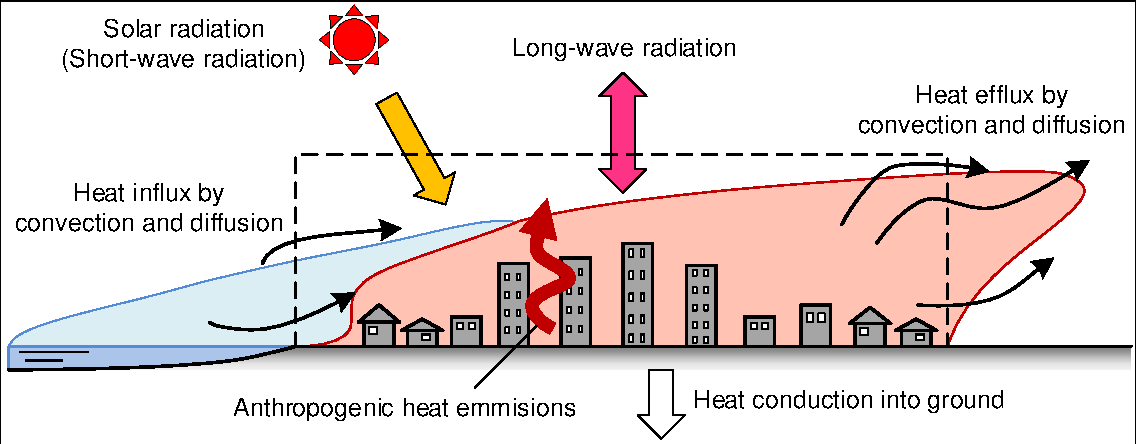
\includegraphics[width=.85\linewidth,trim=2 2 2 2.5,clip]{UHI.pdf}
\caption{Heat balance of the urban surface layer (mainly from Ref. \cite{ooka2011thermal}).}
\end{figure}

Regardless of the inherent uncertainties in predicting future climate and weather patterns, the UHI has been measured and documented throughout the world, including in Washington, DC, New York \cite{hicks2010heat}, Vancouver, Marseille \cite{lee2008vegetated}, London \cite{kolokotroni2012london}, Abu Dhabi \cite{martin2015estimation}, etc. In particular, Crawley \cite{crawley2008estimating} studied the UHI effect on an office building and suggested that the corresponding energy consumption could be modified between 5\% (increase in summer) and 10\% (decrease in winter). In order to meet the increasing peak demand in summer, more electricity generation by power plants will lead to higher emissions of VOCs, suspended particulates, and CO$_2$, as well as to aggravation of global warming and formation of harmful smog \cite{gorsevski1998air}. As a result, the UHI could indirectly cause various health problems leading to morbidity, disability, or even death \cite{gabriel2011urban}. Cities must undertake mitigation and adaptation measures to reduce the negative impacts of heat islands on the environment, the economy, and the population. However, aside from the social and economic concerns, developing effective adaptation strategies comes with a large technical challenge since an urban microclimate system comprises very complex physical relationships between many elements that may interact with each other \cite{masson2014adapting}. A good understanding of the mechanism and characteristics of UHI is thus a prerequisite for decision makers to identify and adopt reliable sustainability options, particularly during the design of new or renovated neighborhood areas.



\section{The state of the art}\label{ch1:opts}

\subsection{Urban-scale simulation model}
This pressing need motivates many energy and environment research communities to expand their scope to the urban realm \cite{reinhart2016urban}. Great efforts have been made to incorporate the UHI effect into thermal simulations \cite{salamanca2010new, crawley2008estimating, oxizidis2008computational}. In addition, some researchers have started to look at the physical behavior or causal factors of urban climate change and heat island effect via mesoscale computational fluid dynamics (CFD) simulations \cite{li2013multi}, analytical and empirical algorithms \cite{ignatius2015urban}, and physics-based urban canopy models \cite{lee2008vegetated}. As different models are developed for different uses, different spatial scales need to be clearly defined and different simulation models need to be elaborated in terms of their capabilities to predict corresponding energy and environmental conditions. Although the mesoscale models are regarded as state-of-the-art in atmospheric weather predictions \cite{roth2007review}, their applications still remain limited due to high computational cost and lack of boundary condition data.

As an alternative, Bueno et al. \cite{bueno2013urban} proposed and developed the Urban Weather Generator (UWG) to quickly estimate the UHI effect in the urban canopy layer and produce neighborhood-specific weather files, using the meteorological data measured at weather stations located in an open area outside the city. The UWG can also be considered as an offline bottom-up model to evaluate the building energy consumption at the neighborhood-to-city scale. It has been validated in Toulouse (France), Basel (Switzerland) \cite{bueno2013urban}, Singapore \cite{bueno2014computationally}, and Boston (USA) \cite{nakano2015urban}. With continuous improvements and updates \cite{yang2016curious}, the UWG has the potential to be a promising urban microclimate simulation engine that shows satisfactory performance with exceptionally low computational requirements.

However, despite the positive progress, simulation practice to date has only penetrated a small fraction of professional communities within the AEC industry. One recognized obstacle is the discrepancy, sometimes significant, between actual and predicted values. In general, prognostic law-driven models \cite{saltelli2008global} involve a suite of simplified physical relations describing the way various component disturbances (from system operation, human activity, material property, etc.) interact with each other and influence the aggregate physical behavior. Within these equations, both differential and algebraic, hundreds or even thousands of parameters exist. It is common for an engineer to make ad-hoc estimates for these parameters based on limited engineering knowledge, past user experience, and an abundance of trial and error. As a result, even though many inputs seem empirically validated, the simulated output could be far from the real scenario. It is ironic that at the time when simulation is the most popular, parameters of simulation may be the least reliable, which inevitably reduces the confidence of simulated results and curtails the use of simulation models to some extent. It is hence necessary to match simulation with measurement, a process called ``model calibration.''

\subsection{Model uncertainty and sensitivity}

Although some studies use calibrated models, their underlying calibration techniques are unclear. In order to dive deeper into model calibration, it is important to consider ``model uncertainty'' \cite{hopfe2011uncertainty}. Validation of a complex-system model is notoriously difficult, especially when the purpose of the model is to look at some non-observable or unmeasured physical behavior. The reason stems from the fact that closed-loop simulations usually represent major simplifications and constraints. That is to say, ``\textit{the portion of the world captured by the model is an arbitrary `enclosure' of an otherwise open, interconnected system}'' \cite{rosen1991life}. Model errors are mainly caused by difficulties in capturing how exactly a system operates, due to software limitations and inaccurate parameter descriptions that cannot be completely modeled a priori. The input parameters are often calibrated manually by an expert, which may require days or weeks of work depending on model complexity. A commonly observed method tunes some specific parameters until the result meets an acceptance criterion without any uncertainty analysis.

Uncertainty quantification is often time-consuming and requires additional efforts in the overall design and/or retrofit phase of an engineering system, but can provide more robust decisions. However, not all the modeled aspects have the same level of importance and not every input parameter offers the same contribution to error propagation. As a result, uncertainty analysis is usually coupled with sensitivity analysis to measure the relative importance of various input parameters \cite{tian2013review}. In general, a single simulation only evaluates one single point in the parameter space without taking uncertainties into account. Consequently, building designers or city planners often perform manual parametric simulations varying one factor at a time, which is referred to as local analysis. This is why some cynics would say that ``\textit{models can be made to conclude anything provided that suitable assumptions are fed into them}'' \cite{economist1998fallout}. As many inputs in the model are associated with some degree of uncertainty, due to changeable conditions or lack of knowledge about the exact value, sensitivity analysis of model parameters plays an important role in the simulation process in order to achieve valuable information and increase model confidence.

Sensitivity analysis (SA), presented by Saltelli et al. \cite{saltelli2004sensitivity}, is a measure of the effect of an input on the output. In general, given the input uncertainties, one is able to assess the uncertainty in the model response (uncertainty analysis), and eventually to identify the inputs that contribute most to that uncertainty (sensitivity analysis). Thus, SA can be of tremendous help in subsequent model analysis, including simulation-based optimization \cite{nguyen2014review}, meta-model analysis \cite{mao2016towards}, automatic model calibration \cite{heo2012calibration}, etc. The SA methods can generally be divided into local and global approaches \cite{saltelli2004sensitivity}. The local methods require fewer computations but are ill-suited for complex systems. The global methods are regarded as more versatile to handle non-linear, non-additive, and non-monotonic systems \cite{tian2013review}.

A brief literature review suggests that the global SA has been widely applied in building thermal simulations \cite{macdonald2002quantifying, heiselberg2009application, de2009identification, eisenhower2012uncertainty, nguyen2015performance, menberg2016sensitivity}. In addition, some researchers have started to look at the causal factors of urban microclimate and heat island via parametric studies \cite{salamanca2010new, lee2008vegetated, martin2015estimation, bueno2013urban, nakano2015urban, hamdi2008inclusion}. However, to the author's best knowledge, there is nearly no related work on performing the global SA in urban microclimate models with respect to a large multiplicity of factors. This is because the global SA approaches are so computationally expensive that most urban-scale simulations cannot afford them. Fortunately, with acceptable performances and exceptionally low computational requirements, the UWG could enable a first step toward the exploration of the global design space with various input parameters in urban simulations. Once the ``weak'' parameters are determined by SA, they could be set at nominal values, thereby reducing the parameter space and increasing the calibration efficiency. The remaining influential input set is considered by a more rigorous calibration process.

\subsection{Optimization-aided model calibration}

Given the evidence that manually tuning the parameters can be viewed as an optimization process, it is natural to think about using computers to implement calibration in automatic or semi-automatic means via optimization algorithms. Simulation-based optimization -- wherein a simulation model is embedded in the optimization -- has been increasingly applied in the building science community through mathematical and statistical methods to assist design analysis \cite{nguyen2014review, evins2013review, machairas2014algorithms} and model calibration \cite{reddy2006literature, coakley2014review, fabrizio2015methodologies}. A pioneering study was conducted by Wright \cite{wright1986optimised} in the 1980s, while the number of optimization-related papers has sharply increased since 2005 \cite{nguyen2014review}. Many open-source tools, such as the \textsc{GenOpt} by Wetter \cite{wetter2009generic}, are now available to provide the capabilities of coupling various building performance simulations to effectively support optimization.

Generally speaking, an objective performance function is formulated to define a max/min target, while some constraint functions are employed to reduce the possibility of deviating too far from the reality. Since the performance function asso-ciated with building or urban thermal-physical behavior is usually discontinuous, non-differentiable, multi-modal, and locally-flat \cite{wetter2004convergent}, traditional gradient-based algorithms cannot successfully search the whole parameter space. On the other hand, heuristic-based algorithms (e.g., evolutionary algorithm) have been frequently used in building or urban performance optimization, mainly owing to their abilities to obtain good solutions with some degree of efficiency and robustness. In particular, a brief literature review indicates that heuristic-based algorithms can perform reliable calibration for building energy models \cite{robertson2015reduced, yang2016automated, ruiz2016genetic, ruiz2017analysis}. To the author's best knowledge, there is nearly no work on performing optimization-based calibration of physics-based urban microclimate models, due partly to the expensive computational costs.

At the current stage, calibration still relies to some extent on expert judgment and engineering experience (e.g., in the selection of candidate inputs). So, we recognize that the computer is more likely to act as a supplement to optimize and accelerate the calibration by transforming manual adjustment into automatic tuning. However, application of numerical optimization in the calibration process, while abstracting the physical objective as a tractable mathematical problem, inevitably neglects some real physical details in the constraint(s). Indiscriminant use could result in mathematical match but physical mismatch, which is why some researchers would criticize such methodology. This naturally necessitates the incorporation of uncertainty analysis after calibration to test reliability.

Finally, although simulation-based optimization has been actively discussed, one practical concern is the computation time. A typical model optimization could take days or weeks of computation to find optimal or near-optimal solutions. Given the time-constrained nature of engineering applications, it is necessary to develop novel optimization methods that are able to find high-quality solutions as quickly as possible.

\section{The goal}

This study was initiated with the intention to account for uncertainty in developing more coherent and integrated strategies concerning the energy and environmental issues in the urban system. The overall goal of this thesis is to identify a general methodology to the topic of automatic model calibration and apply it to an urban microclimate system. Essentially, the proposed ideas involve various concepts and methods borrowed from allied scientific disciplines in a more mathematical and statistical point of view. Corresponding analysis builds upon the newest Urban Weather Generator (UWG) to present a deep look into an existing district area located in downtown Abu Dhabi (UAE).

The core of the thesis is divided into \textit{two} parts, which correspond to two journal publications \cite{mao2017global,mao2018optimization} that have come out of this research. The first part is devoted to global sensitivity analysis, which is used to determine the relative impacts of input parameters on estimates of the urban outdoor air temperature. The second part is devoted to optimization-aided model calibration, which is used to auto-tune the selected input parameters so that the UWG model can represent the urban microclimate as precisely as possible. To the author's best knowledge, this is to date the first time to perform global sensitivity analysis and automatic calibration on physics-based urban microclimate models.

\textbf{Chapter 1} overviews the state of the art in urban microclimate simulation research and states the thesis goal. \textbf{Chapter 2} introduces the basic mechanism and major updates of the newest UWG for urban microclimate simulation. \textbf{Chapter 3} illustrates a baseline model of the selected case study for the proposed methodologies detailed in \textbf{Chapter 4}. In particular, we have developed a global regression-based sensitivity analysis, a Monte Carlo filtering technique, and an online hyper-heuristic evolutionary algorithm for the current research. Finally, results and discussions are provided in \textbf{Chapter 5}, and the corresponding conclusions and prospects for future work are outlined in \textbf{Chapter 6}.

The final achievement of this study is expected to be helpful in using simulation-based analysis as a deeper basis for providing the tool, guideline, recommendation, best-practice example, and background information to practitioners and researchers in the field of building and/or urban system study. In this sense, a modeling approach that is able to robustly integrate field measurements and computer simulations has the potential to significantly improve the way buildings and/or cities are designed and operated. This research aims to represent an initial step toward such promising vision.

\chapter{Urban Weather Generator}

\AddToShipoutPictureBG*{%
  \AtPageUpperLeft{%
    \hspace*{18.35cm}%
    \raisebox{-3cm}{%
      \makebox[0pt][r]{\parbox{\textwidth}{\begin{flushright}\textit{``All models are wrong, but some are useful.''}\\
      George Box\end{flushright}}}
}}}%

In order to capture the UHI effect and to simulate the microclimate condition, the Urban Weather Generator (UWG) was developed by Bueno et al. \cite{bueno2013urban} as a stand-alone program to map a reference weather file to the estimated conditions at a neighborhood scale based on the specific urban area characteristics.

\section{Program introduction}

The wisdom of UWG comes from the fact that many communities do not have access to the microclimate information from local experimental measurements and mesoscale simulation results, while the rural meteorological information can be easily found in currently available weather files. Starting with the rural weather data provided in the EPW format and the urban characteristics, the UWG outputs the simulated urban weather data (during either an entire calendar year or just a subset thereof) that can be readily used in the EPW format.

\begin{figure}
\centering
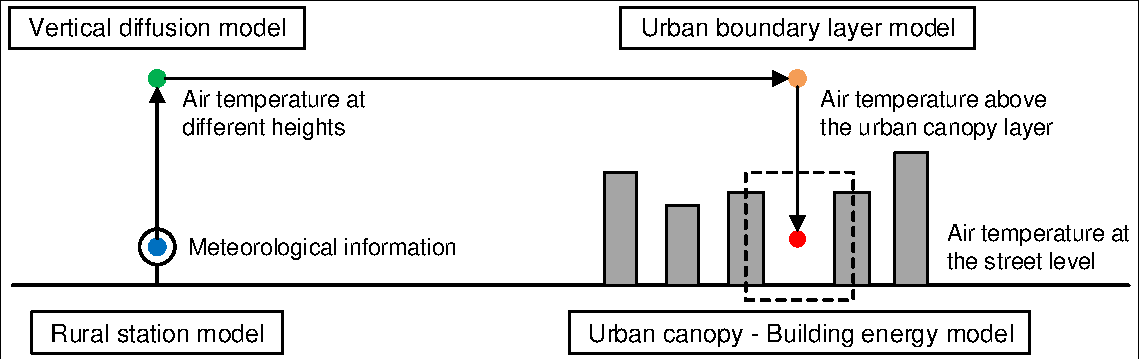
\includegraphics[width=.8\linewidth,trim=2 2 2 2,clip]{UWG.pdf}
\caption{Four coupled models in the UWG (mainly from Ref. \cite{bueno2013urban}).}
\end{figure}

As shown in \textbf{Figure 2-1}, the UWG consists of four coupled models: the rural station model (RSM), the vertical diffusion model (VDM), the urban boundary layer model (UBLM), and the urban canopy-building energy model (UC-BEM). Detailed physical mechanisms of these models can be found in Refs. \cite{bueno2013urban, bueno2013calculation}. Originally written in \textsc{Matlab}, following update of the UWG program further includes XML \cite{nakano2015urban} and Excel \cite{yang2016curious} interfaces to allow flexibility in input formats of the urban characteristics. General workflow of the UWG program is depicted in \textbf{Figure 2-2}. The version used in this thesis is a macro-enabled Excel interface along with compiled \textsc{Matlab} scripts of the UWG as a standalone urban microclimate simulation package.

\begin{figure}
\centering
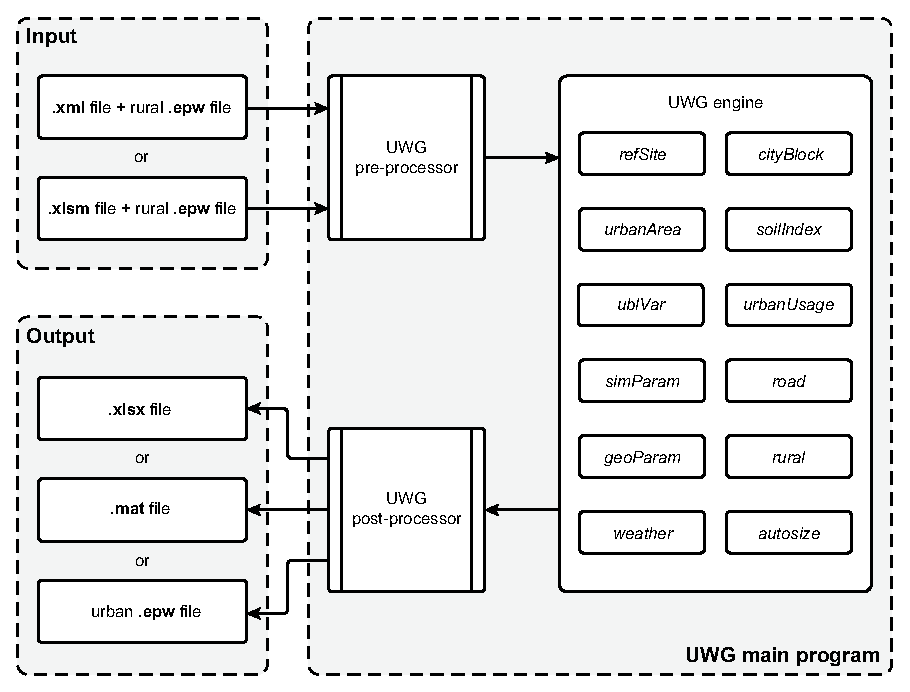
\includegraphics[width=.825\linewidth]{UWGEngine.eps}
\caption{General workflow of the UWG program (mainly from Ref. \cite{yang2016curious}).}
\end{figure}

Based on the main UWG code, \textsc{Dragonfly} is a new component for Grasshopper and Rhino that allows users to model and estimate large-scale climate phenomena, such as the UHI effect. This is accomplished with the help of several urban thermal simulation engines, including the UWG and CitySim \cite{robinson2009citysim}. It also links to several climate-related datasets such as the Hadley Global Circulation Model (for climate change projections) and to several satellite image datasets such as the Landset and MODIS from NASA. The \textsc{Dragonfly} program intends to make many large-scale climate variables accessible to the visual scripting interface of Grasshopper as well as the 3D visualization interface of Rhino. The latest executable tool and program code (in Python) are currently maintained by Mackey et al. \cite{mackey2015dragonfly} on GitHub.

\section{Program update}

Since the previous version in 2014 \cite{bueno2014computationally}, the UWG has been updated in 2016 \cite{yang2016curious}, especially for the urban boundary layer model and the urban canopy-building energy model, with the purpose of making it more physically sound and more capable to handle increasingly detailed building definition. Major updated features of the current UWG are re-emphasized and described below.

\subsection{Urban canopy model}

Based on the Town Energy Balance (TEB) scheme proposed by Masson \cite{masson2000physically}, the UWG maps the 3D urban geometry to a 2D canyon model consisting of a wall, roof, and road, representative of the average urban characteristics. While the previous version bounded the canyon volume by twice the building height, the urban boundary layer (UBL) in the new version extends down to the top of the building. All heat released from the roof is assumed to directly enter the UBL. This makes the formulation more consistent with the original TEB scheme.

The direct solar radiation in the new version is also updated for numerical stability. According to Masson \cite{masson2000physically}, their fractions are given by:

\begin{equation}
K_{w,dir}=\min \Bigl\{ \frac{w_r}{h_{bld}} (\frac{1}{2} - \frac{\theta_0}{\pi}) + \frac{1}{\pi} \tan (\lambda)(1 - \cos (\theta_0)),\; 1 \Bigr\}\,,
\end{equation}

\begin{equation}
K_{r,dir}=\min \Bigl\{ \frac{2\theta_0}{\pi} - \frac{2}{\pi} \frac{h_{bld}}{w_r} \tan (\lambda)(1 - \cos (\theta_0)),\; 1 - 2 r_{aspect} K_{w,dir} \Bigr\}\,,
\end{equation}

\vspace{15pt}
\noindent where $K_{w,dir}$ is capped to 1 as the sun approaches the horizon.

While Masson defined these terms to scale the direct solar radiation received by a horizontal surface, the value specified in a standard EPW file is the direct normal radiation, namely the solar radiation received by a surface perpendicular to the sunlight direction. This indicates that the previous model had a slightly excessive solar gain. Thus, the direct solar radiation in the newest UWG is modified as:
\vspace{12pt}
\begin{equation}
S_{hor,dir} = S_{norm,dir} \cos (\lambda)\,.
\end{equation}

\vspace{9pt}
In terms of the infrared radiation (IR) exchange, the previous version seemed to over-estimate the IR absorption by bodies of air \cite{fenn1985optical}. To correct this over-estimation, the air is now assumed to be essentially transparent to the long-wavelength (LW) radiation emitted from its boundary surfaces. This assumption has been validated with MODTRAN simulations \cite{yang2016curious}, showing that the IR absorption of the air is almost negligible for the thick air bodies (around 1 km) considered in the UWG. Thus, the net LW heat exchanges with the atmosphere for the roof, wall, and road are given as:

\begin{equation}
Q_{LW,roof} = \epsilon_{roof} (Q_{LW,down} - \sigma T^4_{roof})\,,
\end{equation}
\vspace{-1em}
\begin{equation}
\begin{split}
\hspace{-1.5pt} Q_{LW,wall} & = \epsilon_{wall} VF_{wall-sky} (Q_{LW,down} - \sigma T^4_{wall}) \\
& \hspace{12pt}+\hspace{3pt} \sigma \epsilon_{road} \epsilon_{wall} VF_{wall-road} (1 - r_{shade}) (T^4_{road} - T^4_{wall})\,,
\end{split}
\end{equation}
\vspace{-0.25em}
\begin{equation}
\begin{split}
\hspace{-1.5pt} Q_{LW,road} & = \epsilon_{road} VF_{road-sky} (1 - r_{shade}) (Q_{LW,down} - \sigma T^4_{road}) \\
& \hspace{12pt}+\hspace{3pt} \sigma \epsilon_{road} \epsilon_{wall} VF_{road-wall} (1 - r_{shade}) (T^4_{wall} - T^4_{road})\,,
\end{split}
\end{equation}

\vspace{21pt}
\noindent where $Q_{LW,down}$ has accounted for the radiative effect due to the water vapor and carbon dioxide contained in the UBL.

Since the latent heat exchange between the four coupled models was not fully considered, Yang \cite{yang2016curious} decided to remove the humidity calculation for canyon in the new version of UWG. This calculation requires consideration of the moisture from vegetation, soil, combustion, nearby bodies of water, etc., and these components have not been precisely modeled in the current UWG. It is also worth noting that the latent heat balance in the urban canyon has not been formally validated \cite{bueno2013urban,bueno2014computationally}. Thus, the absolute humidity in the rural area is assumed the same as that in the urban area, and is then used to calculate the relative humidity for the generated EPW file. When accounting for the solar radiation received by the vegetation, we only consider its sensible portion in the energy balance, subtracting a prescribed latent-energy fraction.

When the urban weather file is generated, the calculated canyon wind speed is included, instead of the rural wind speed used by previous versions. The calculation is detailed in the appendixes of Refs. \cite{bueno2013urban,bueno2014computationally}. In addition, the new UWG incorporates a user-specified hourly schedule for the traffic-generated heat flux, as a counterpart to the schedules defined in the building energy model, to make the simulated diurnal microclimate profile more accurate. Finally, the new version of UWG reads the soil temperatures from the EPW file, and uses these values as the boundary condition to obtain the road layer temperature profile. It is also worth noting that the road elements in the new version are divided into thinner layers (with maximum of 5 cm) so that the surface temperature fluctuation can be captured more precisely.

\subsection{Urban boundary layer model}

The urban boundary layer (UBL) model solves an energy balance for a control volume above the urban canopy layer (UCL) where the boundary conditions can be imposed \cite{bueno2013calculation}. The UBL is considered as a region of well-mixed and isothermal air below a capping inversion.

As explained in \textbf{Subsection 2.2.1}, the IR portion of the energy exchange added in 2014 \cite{bueno2014computationally} is now removed. Thus, the energy balance of the current UBL model remains the same as the original version in 2012 \cite{bueno2013calculation}, defined as:

\begin{equation}
V_{CV} \rho c_v \frac{d\theta_u}{dt} = H_u + \int u_{ref} \rho c_p (\theta_{ref} - \theta_u) dA_f\,,
\end{equation}

\vspace{15pt}
\noindent where the term on the LHS stands for the thermal inertia of the control volume, and the second term on the RHS stands for the advection effect.

The heat exchange at top of the control volume is assumed negligible when the vertical profile of the potential temperature provided by the vertical diffusion model is constant. So, the energy balance of the UBL model is driven only by the heat flux from the bottom or the lateral sides of the volume surface.

The advection effect is driven by either the horizontal flow or the radial urban-breeze circulation where the wind direction is not taken into account. Therefore, the rural weather data seems applicable to large concentric regions surrounding the urban area \cite{hidalgo2010scaling}.


\subsection{Building energy model}

The building energy model approximates the heat balance of the indoor air temperature for each building. For simplicity, the air temperature is assumed uniform within the entire building envelope. As a result, the UWG can capture the building energy operations and calculate the waste heat emissions from HVAC systems, which are the potentially significant sources of heat in the energy balance of an urban canyon.

Whereas the old version only specified the total internal heat load in buildings, the new UWG takes into account the variation in the types of heat loads. As shown in \textbf{Table 2.1}, the updated UWG treats the convective, latent, and radiant heat loads separately. The convective and latent heat exchange is added directly into the indoor air heat balance, while the radiant heat flux is received by the ceiling and floor. The view factors from lights and occupants to the ceiling and floor are assumed close to unity.

\begin{table}[]
\centering
\footnotesize
\caption{Fractions of the internal heat loads.}
\label{my-label}
\begin{tabular}{lllll}
\toprule
                    & Occupancy load & Equipment load & Lighting load & Added to \\ \hline
Convective fraction & 0.5            & 0.5            & 0.3           & Air      \\
Latent fraction     & 0.3            & 0              & 0             & Air      \\
Radiant fraction    & 0.2            & 0.5            & 0.7           & Mass     \\
\bottomrule
\end{tabular}
\vspace{2.5ex}

\raggedright Note: The fraction values are selected based on ASHRAE Handbook -- Fundamentals \cite{handbook2009american}.
\end{table}

To simplify the estimation of various building types at the neighborhood scale, commercial building reference data is imported from the US DOE online database \cite{deru2011us} into a spreadsheet associated with UWG. This allows the users to specify the building types that make up the urban area, instead of modeling all the buildings individually. Accordingly, the updated UWG simulates the hourly schedules of occupancy, lighting, and equipment loads for each building type using the default values provided in the DOE reference building database, with flexible options for user customization. The goal is a better estimation of the building energy use pattern at the urban scale and the temporal sensible heat fluxes released into the surrounding environment. In addition, we consider a single building zone with a generic thermal mass and use the multi-zone-weighted average to calculate the internal heat gain. The simplified building models have been validated against the original models in Ref. \cite{yang2016curious}.

For the heating mechanism in the updated version, the internal heat gain is added into the building control volume based on the heating requirement, instead of based on the supply air temperature and mass flow rate. On the other hand, the cooling demand is determined by a psychrometric model based on the apparatus dew point. If the energy demand is greater than the system capacity, the system capacity is then used to calculate the supply air temperature.

In order to properly size the building elements, detailed information for the case study is determined according to local summaries and then is substituted into the DOE reference building database. As for the thermal properties of the building envelope, if the insulation layer is too thin (less than 1 cm), it will not be modeled in the structural element to avoid solver instability. Such omission will not significantly affect the thermal characteristics of the structure. However, the surface optical properties, such as the albedo and emissivity, are still taken into account.

Finally, while the previous version calculated the waste heat based on the total building energy consumption, the updated version treats the waste heat in more detail. The energy consumed by lights and equipment is considered as the heat flux received by either indoor air or internal surfaces, eventually merging with the canyon air through windows and walls. The waste heat added directly into the canyon is calculated based on the HVAC-related waste heat (with a predetermined fraction), as well as the waste heat from hot water usage and gas consumption\footnote{Assuming that the zones where gas equipment is used are well-ventilated (indicated by exhaust rate for EnergyPlus models), the heat loads of gas equipment are not included in the internal sensible heat loads \cite{yang2016curious}. Hence, similar to space and water heating, a specified fraction of the gas consumption is added to the waste heat from the building(s).}.


\chapter{Baseline urban design}

\AddToShipoutPictureBG*{%
  \AtPageUpperLeft{%
    \hspace*{18.25cm}%
    \raisebox{-3.25cm}{%
      \makebox[0pt][r]{\parbox{\textwidth}{\begin{flushright}\textit{``Scientists investigate that which already is;\\ Engineers create that which has never been.''}\\
      Albert Einstein\end{flushright}}}
}}}%

In this chapter, a baseline model is established based on the newest version of UWG for a typical district in downtown Abu Dhabi (UAE). The baseline model is validated using the measurements in 2016 for the subsequent research.

\section{Case study in Abu Dhabi}

Abu Dhabi has been developed rapidly over the past 60 years. Its climate is characterized by a very hot summer from July to September and a mild winter from December to February. The city experiences an environment with generally high temperatures and insufficient rainfall throughout the year. The K\"{o}ppen climate classification subtype for Abu Dhabi is BWh (tropical and subtropical desert climate).

This case study was conducted in District E3 (see \textbf{Figure 3-1}), which is representative of the large city blocks in downtown Abu Dhabi. The total land area of District E3 is about 193,351 m$^2$. As shown in \textbf{Figure 3-1(b)}, there is a row of high-rise residential, office, and hotel buildings on the outer borders surrounding a number of medium- and low-rise buildings in the inner part. In total, 70 buildings are considered in the baseline model, including 59 residential buildings, five office buildings, three hotels, one mosque, one school, and one hospital. In general, the buildings built in the 1990s have smaller window-to-wall ratios, while the buildings built after 2000 are mostly glazed over the fa\c{c}ade. This makes Abu Dhabi an interesting case with heterogeneous building forms located in a tropical or subtropical climate zone.

\begin{figure}
\centering
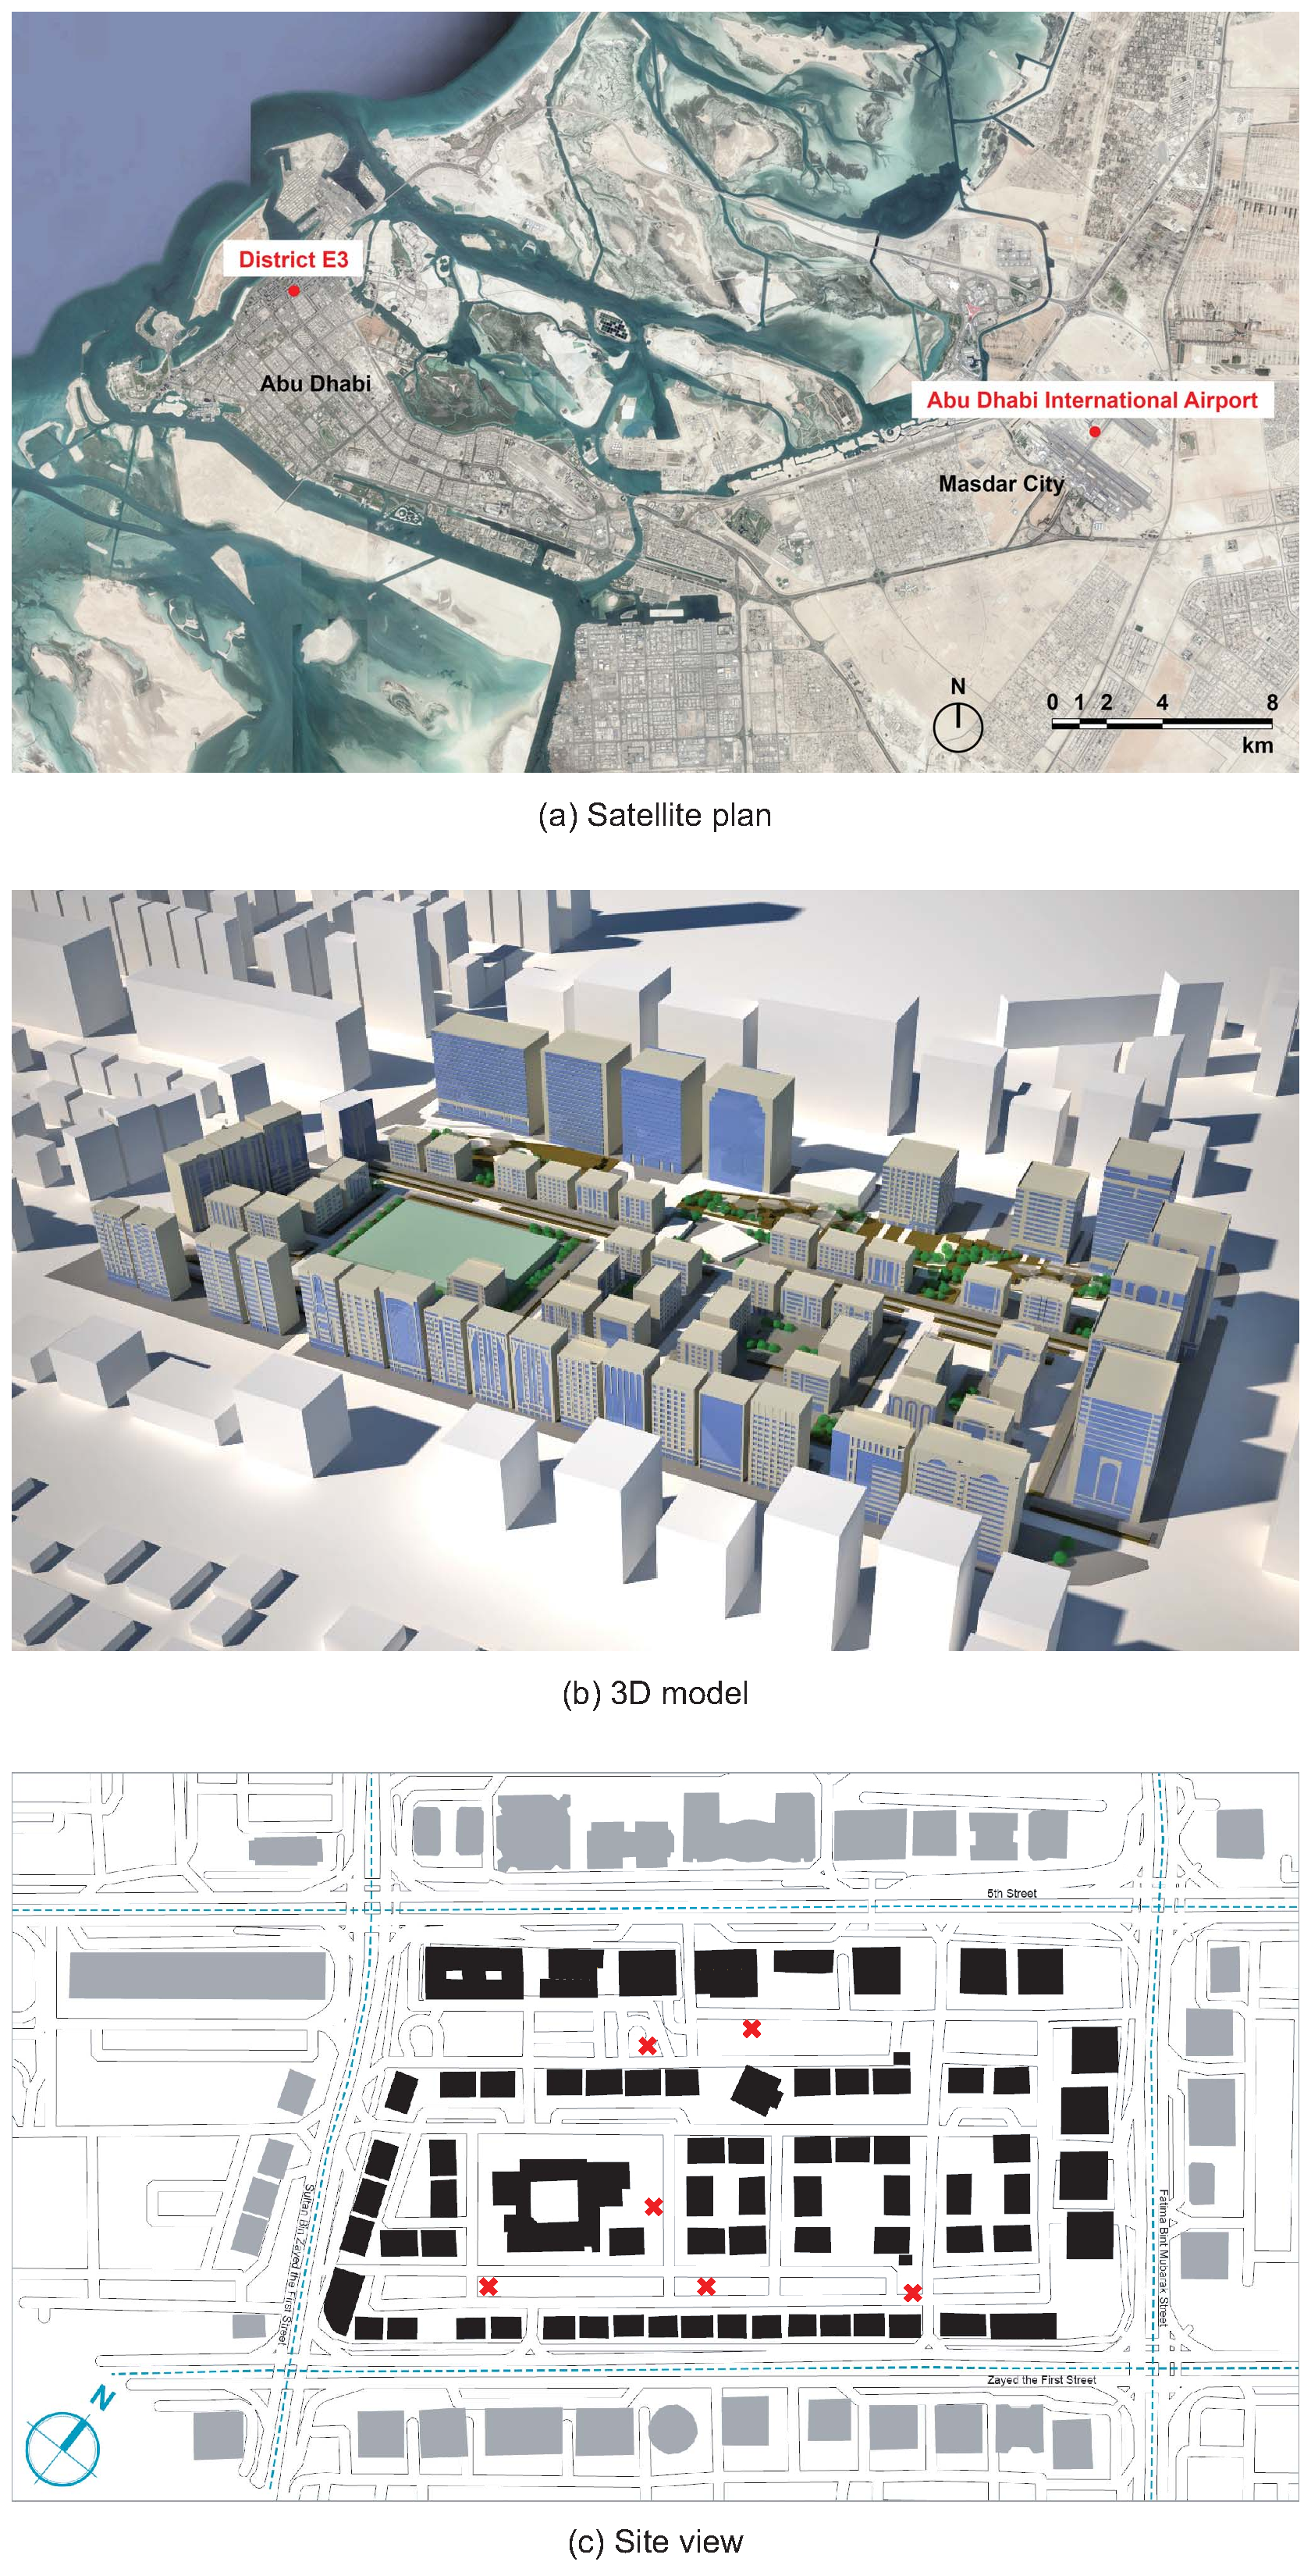
\includegraphics[width=.73\linewidth,trim=1 1 1 1,clip]{DistrictE3.pdf}
\caption{District E3 in downtown Abu Dhabi (UAE).}
\end{figure}

\begin{table}[]
\footnotesize
\begin{center}
\caption{Inputs of the UWG used in the baseline model with field data from District E3 in Abu Dhabi.}
\label{my-label}
\begin{tabular}{ll}
\toprule
Parameter                                    & Setting                 \\ \hline 
\rule{0pt}{4ex} \textit{General information} \vspace{6pt}                &                         \\
\hspace{12pt}Location                                     & Abu Dhabi               \\
\hspace{12pt}Latitude                                     & 24.490$^{\circ}$                 \\
\hspace{12pt}Longitude                                    & 54.366$^{\circ}$                 \\
\hspace{12pt}Simulation time-step                         & 300 s                   \\
\hspace{12pt}Weather data time-step                       & 3600 s                  \\
\hspace{12pt}Simulation period for validation                            & 10/01/2016 -- 10/07/2016 \\
                                             & 11/01/2016 -- 11/07/2016 \\
                                             & 12/01/2016 -- 12/07/2016 \vspace{6pt} \\
\vspace{6pt}\textit{Meteorological factors}              &                         \\
\hspace{12pt}Daytime urban boundary layer height          & 700 m                   \\
\hspace{12pt}Nighttime urban boundary layer height        & 80 m                    \\
\hspace{12pt}Reference height of the VDM                  & 150 m                   \\
\hspace{12pt}RSM temperature reference height             & 10 m                    \\
\hspace{12pt}RSM wind reference height                    & 10 m                    \\
\hspace{12pt}Circulation coefficient                      & 1.2                     \\
\hspace{12pt}UCM-UBL exchange coefficient                 & 0.3                     \\
\hspace{12pt}Heat flux threshold for daytime conditions   & 200 W m$^{-2}$               \\
\hspace{12pt}Heat flux threshold for nighttime conditions & 50 W m$^{-2}$                \\
\hspace{12pt}Minimum wind velocity                        & 0.1 m s$^{-1}$               \\
\hspace{12pt}Rural average obstacle height \vspace{6pt}               & 0.1 m                   \\
\vspace{6pt}\textit{Urban characteristics}               &                         \\
\hspace{12pt}Average building height                      & 35 m                    \\
\hspace{12pt}Fraction of waste heat into canyon           & 0.3                     \\
\hspace{12pt}Building density                             & 0.24                    \\
\hspace{12pt}Vertical-to-horizontal ratio                 & 2.2                     \\
\hspace{12pt}Urban area characteristic length             & 1000 m                  \\
\hspace{12pt}Road albedo                                  & 0.165                   \\
\hspace{12pt}Pavement thickness                           & 1.25 m                  \\
\hspace{12pt}Traffic sensible anthropogenic heat (peak)   & 19.6 W m$^{-2}$              \\
\hspace{12pt}Traffic latent anthropogenic heat (peak) \vspace{6pt}    & 2.0 W m$^{-2}$               \\
\vspace{6pt}\textit{Vegetation variables}                &                         \\
\hspace{12pt}Urban vegetation coverage                    & 0.01                    \\
\hspace{12pt}Urban tree coverage                          & 0.01                    \\
\hspace{12pt}Start month of vegetation participation      & January                 \\
\hspace{12pt}End month of vegetation participation        & December                \\
\hspace{12pt}Vegetation albedo                            & 0.25                    \\
\hspace{12pt}Latent fraction of grass                     & 0.6                     \\
\hspace{12pt}Latent fraction of tree                      & 0.7                     \\
\hspace{12pt}Rural vegetation coverage                    & 0.01                    \\
\bottomrule
\end{tabular}
\end{center}
Note: Detailed physical definition of the parameters can be found in Refs. \cite{bueno2013urban,bueno2013calculation}. In particular, Ref. \cite{bueno2013urban} illustrates the parameters in the rural station model (RSM) and urban canopy-building energy model (UC-BEM), while Ref. \cite{bueno2013calculation} illustrates the parameters in the vertical diffusion model (VDM) and urban boundary layer model (UBLM).
\end{table}


\begin{table}[]
\footnotesize
\begin{center}
\caption{Building parameters for the detailed model (DM) in the UWG.}
\label{my-label}
\makebox[\linewidth]{
\begin{tabular}{lllllll}
\toprule
Building parameter              & Residential & Hotel  & Office  & Mosque & School & Hospital \\ \hline
Total floor area (m$^2$)           & 382,086     & 99,666 & 140,886 & 2070   & 15,159 & 10,589   \\
Glazing ratio                   & 0.39        & 0.75   & 0.72    & 0.11   & 0.34   & 0.90      \\
Wall U-value (W m$^{-2}$ K$^{-1}$)        & 2.70         & 2.27   & 1.71    & 2.70    & 2.70    & 1.71     \\
Roof U-value (W m$^{-2}$ K$^{-1}$)        & 0.74        & 0.74   & 0.53    & 0.74   & 0.74   & 0.53     \\
Window U-value (W m$^{-2}$ K$^{-1}$)      & 3.88        & 2.40    & 2.40     & 3.88   & 3.88   & 2.40      \\
Window SHGC                     & 0.75        & 0.36   & 0.36    & 0.75   & 0.75   & 0.36     \\
Infiltration rate (ACH)         & 0.75        & 0.50    & 0.30     & 0.75   & 0.75   & 0.20      \\
Lighting load density (W m$^{-2}$)   & 8           & 10     & 12      & 8      & 15     & 15       \\
Equipment load density (W m$^{-2}$)  & 12          & 13     & 15      & 5      & 10     & 15       \\
Occupancy density (m$^2$ person$^{-1}$) & 25          & 10     & 10      & 10     & 8      & 15       \\
Indoor air temperature set point ($^{\circ}$C)       & 22          & 22     & 22      & 22     & 22     & 22       \\
Chiller COP                     & 2.5         & 2.5    & 2.5     & 2.5    & 2.5    & 2.5      \\
\bottomrule
\end{tabular}
}
\end{center}
Note: The values are determined based on the corresponding data taken from the local building design/energy codes provided by the Abu Dhabi Municipality (via personal contact), the on-site survey, and the prevailing engineering practices \cite{martin2015estimation,deru2011us,radhi2009evaluating,afshari2014life}.
\end{table}

The parameters used for establishing the baseline model can be categorized into four groups: meteorological factors, urban characteristics, vegetation variables, and building systems. Since detailed data collection efforts on building properties would become impractical at the urban scale, it is necessary to abstract a building stock into ``building archetypes.'' While such division is of tremendous importance for modeling reliability, the process usually remains \textit{ad hoc} based on generic assumptions. In our case study, the descriptions of the baseline model are based on careful selections of typical design and construction with corresponding data taken from the Abu Dhabi Municipality (via personal contact) and prevailing engineering practices \cite{martin2015estimation,bueno2013urban,bueno2014computationally,bueno2013calculation,deru2011us,radhi2009evaluating,afshari2014life}. A summary of the key input parameters is shown in \textbf{Tables 3.1 and 3.2}. The structural elements of the DOE reference buildings based on the Miami climate are modified according to the current building descriptions, since the climate in Miami is quite similar to that in Abu Dhabi.

\section{Model of anthropogenic heat flux}

In urban studies, anthropogenic heat flux is defined as the heat released due to human activities \cite{oke2002boundary}. According to Sailor \cite{sailor2011review}, it generally includes the heat from building operation, traffic vehicles, and human metabolism.

A methodology is proposed to evaluate the aggregated effect of building energy models on the outdoor microclimate conditions in the subsequent uncertainty/sensi-tivity analysis and model calibration. The underlying expectation is that the average building in a specific urban area is more thermally homogeneous and generic than each particular building. Two models of District E3 with different levels of detail are compared via UWG. The first model, referred to as the detailed model (DM), includes the exact information for the six building archetypes extracted from available resources. The second model, referred to as the averaged model (AM), maintains the assumptions of the building energy model but considers only one building archetype using weighted average values. The key parameters of the building geometry, energy load, and HVAC system are all set as weighted averages based on corresponding area or volume. We assume that the schedules for each building prototype cannot be averaged and thus remain unchanged. This method is adopted only if the objective is to evaluate the overall energy consumption of a neighborhood area, rather than the energy performance of a specific building. \textbf{Tables 3.2 and 3.3} summarize the parameters in DM and AM, respectively.

\begin{table}[]
\footnotesize
\begin{center}
\caption{Building parameters for the averaged model (AM) in the UWG.}
\label{my-label}
\begin{tabular}{ll}
\toprule
Building parameter                    & Weighted average \\ \hline
Glazing ratio                         & 0.48             \\
Wall U-value (W m$^{-2}$ K$^{-1}$)              & 2.5              \\
Roof U-value (W m$^{-2}$ K$^{-1}$)              & 0.7              \\
Window U-value (W m$^{-2}$ K$^{-1}$)            & 3.25             \\
Window SHGC                           & 0.58             \\
Infiltration rate (ACH)               & 0.6              \\
Lighting load density (W m$^{-2}$)         & 10               \\
Equipment load density (W m$^{-2}$)        & 13               \\
Occupancy density (m$^2$ person$^{-1}$)       & 19               \\
Indoor air temperature set point ($^{\circ}$C) & 22               \\
Chiller COP                           & 2.5              \\
\bottomrule
\end{tabular}
\end{center}
Note: The wall-, window-, and roof-related parameters are averaged based on the wall, window, and roof area, respectively. The internal heat gains are averaged based on the floor area. The infiltration level is averaged based on the building volume.
\end{table}

In the meantime, there has been a completed research project working exclusively on quantifying the traffic-related anthropogenic heat in District E3 \cite{afshari2017estimation}, since the outdoor metabolic heat is negligible and the building-related waste heat can be calculated by the UWG. The novelty of the method lies in the assumption that the air quality measurements can be a proxy for traffic intensity. In particular, the BTEX (Benzene, Toluene, Ethylbenzene, and m-, p-, o-Xylenes) concentration levels appear strongly correlated with the traffic intensity \cite{afshari2017estimation}.

The normalized diurnal profiles of the traffic intensity were derived using the BTEX concentrations measured in a downtown air quality monitoring station near District E3 during calendar year 2012. We neglect the seasonal dependence and focus on the variance on a daily basis, since the diurnal average BTEX profile is not sensitive to seasons. As shown in \textbf{Figure 3-2}, the Friday profile is quite different from the workday profile, whereas Saturdays present wide similarities with workdays. There are two peaks at 9 am and 10 pm and one minimum at 5 am in the workday diurnal profile. The Friday profile also peaks at 10 pm, while the high values persist during the nighttime. Such differences can be explained by cultural and climatic reasons. In Abu Dhabi, it is worth noting that the weekend is Friday and Saturday; Friday is the weekly Muslim holy day, a day of public worship.

\begin{figure}
\centering
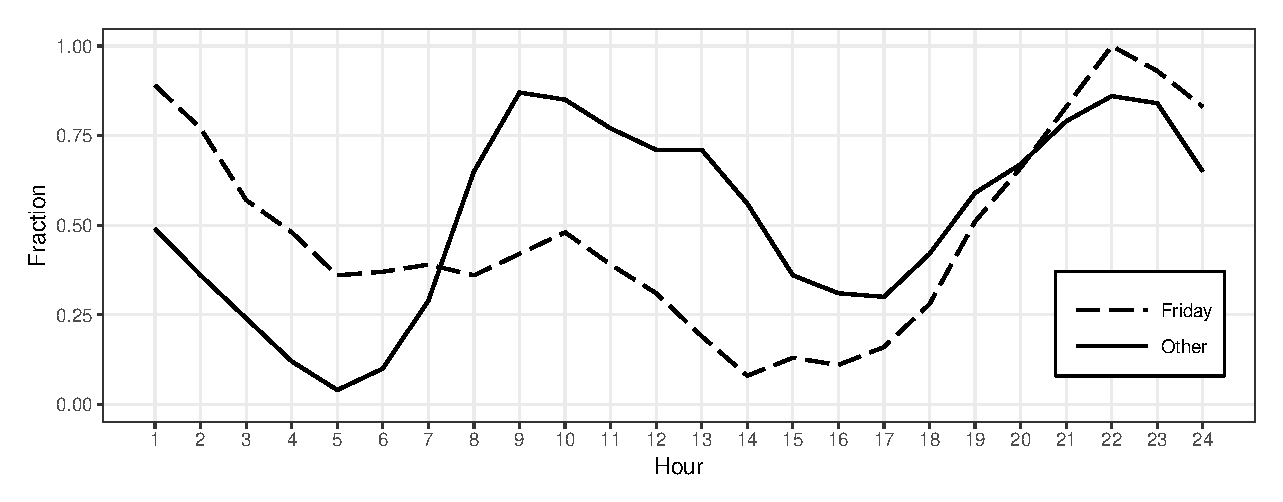
\includegraphics[width=.8\linewidth]{TrafficHeat.eps}
\caption{Normalized diurnal profile of the average traffic intensity in Abu Dhabi based on the BTEX concentration (mainly from Ref. \cite{afshari2017estimation}).}
\end{figure}

The normalized profile has been calibrated using either a bottom-up method based on high-resolution satellite images of the traffic intensity, or a top-down method based on average macro-economic and demographic variables \cite{afshari2017estimation}. Both methods have been applied and the results were quite similar. The peak traffic sensible anthropogenic heat load for the diurnal profile is 19.6 W/m$^2$, based on the full site. This is quite consistent with the result produced by Quah and Roth \cite{quah2012diurnal} in Singapore. The peak latent heat load due to motorized traffic is estimated to be 2.0 W/m$^2$.

\section{Reference and sensor data for validation}

The rural reference weather data used for the baseline model is taken from the Masdar Institute Field Station (24.436N, 54.612E), an isolated laboratory building in Masdar City. The station was built near the Abu Dhabi International Airport, 28 km from the downtown area (see \textbf{Figure 3-1(a)}). The rural station is basically surrounded by deserts connecting Abu Dhabi, Dubai, and Al Ain. Due to regular maintenance to ensure data quality, the measured data during calendar year 2016 is used for running the UWG to validate the baseline model. As shown in \textbf{Figure 3-3}, Abu Dhabi has a maximum temperature in August 2016 (about 47.3 $^{\circ}$C) and a minimum temperature in February 2016 (about 8.7 $^{\circ}$C).

\begin{figure}
\centering
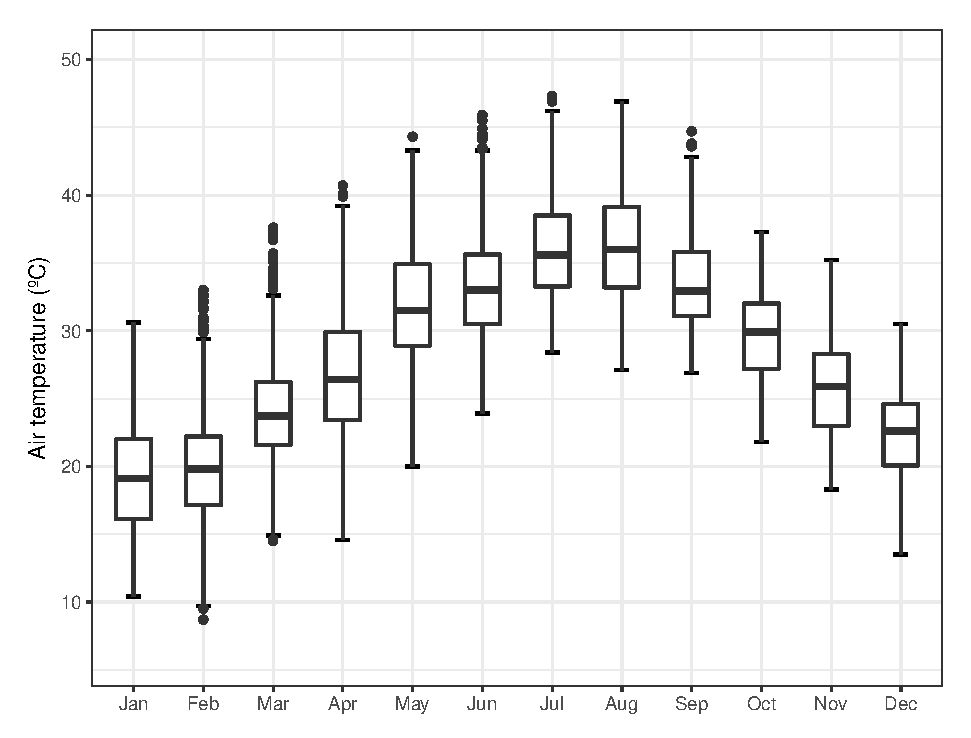
\includegraphics[width=.6\linewidth]{Weather2016.eps}
\caption{Monthly outdoor air temperature measured at the rural station in Abu Dhabi during 2016.}
\end{figure}

Temperature observations from installed urban sensors are compared with the predicted values by the UWG baseline model. In fall 2016, several arrays of sensors were attached to six lamp poles in District E3 at different sites, representing a range of land usages, morphological parameters, building operations, etc. Each sensor array consists of temperature measurements (at 3, 4, 5.5, 7, and 8.5 m), relative humidity measurements (at 3 m), and wind measurements (at 6 m, only available in four of the six stations). The sensors were inspected against each other before deployment to ensure relative accuracy of readings.

We use the data measured in 2016 from three of the calibrated sensors that present consistent performances for validating the baseline model. The corresponding locations in (latitude, longitude) of the three sensors are (24.4902$^{\circ}$, 54.3654$^{\circ}$), (24.4894$^{\circ}$, 54.3663$^{\circ}$), and (24.4907$^{\circ}$, 54.3660$^{\circ}$). In particular, the temperature observations at 8.5 m are selected for the subsequent comparison, since they are more suitable to validate the current UWG outputs for this case study (given that the average building height is 35 m).

\section{Prediction of urban outdoor air temperature}

\textbf{Figure 3-4} compares the weekly-average profiles of rural and urban outdoor air temperature calculated by the model from October to December 2016. The diurnal pattern of UHI is characterized by a slightly cooler temperature in the urban area than in the rural area during the late morning, and a relatively warmer temperature from the afternoon to the early morning the next day. The urban-rural temperature differences are more intense in the early morning. This is quite consistent with the results from previous studies \cite{bueno2013urban,bueno2014computationally,oke2002boundary}. Generally speaking, due to the aggregate effect of the whole city, the UHI cannot be neglected in Abu Dhabi for the assessment of either thermal comfort or energy consumption.

\begin{figure}
\centering
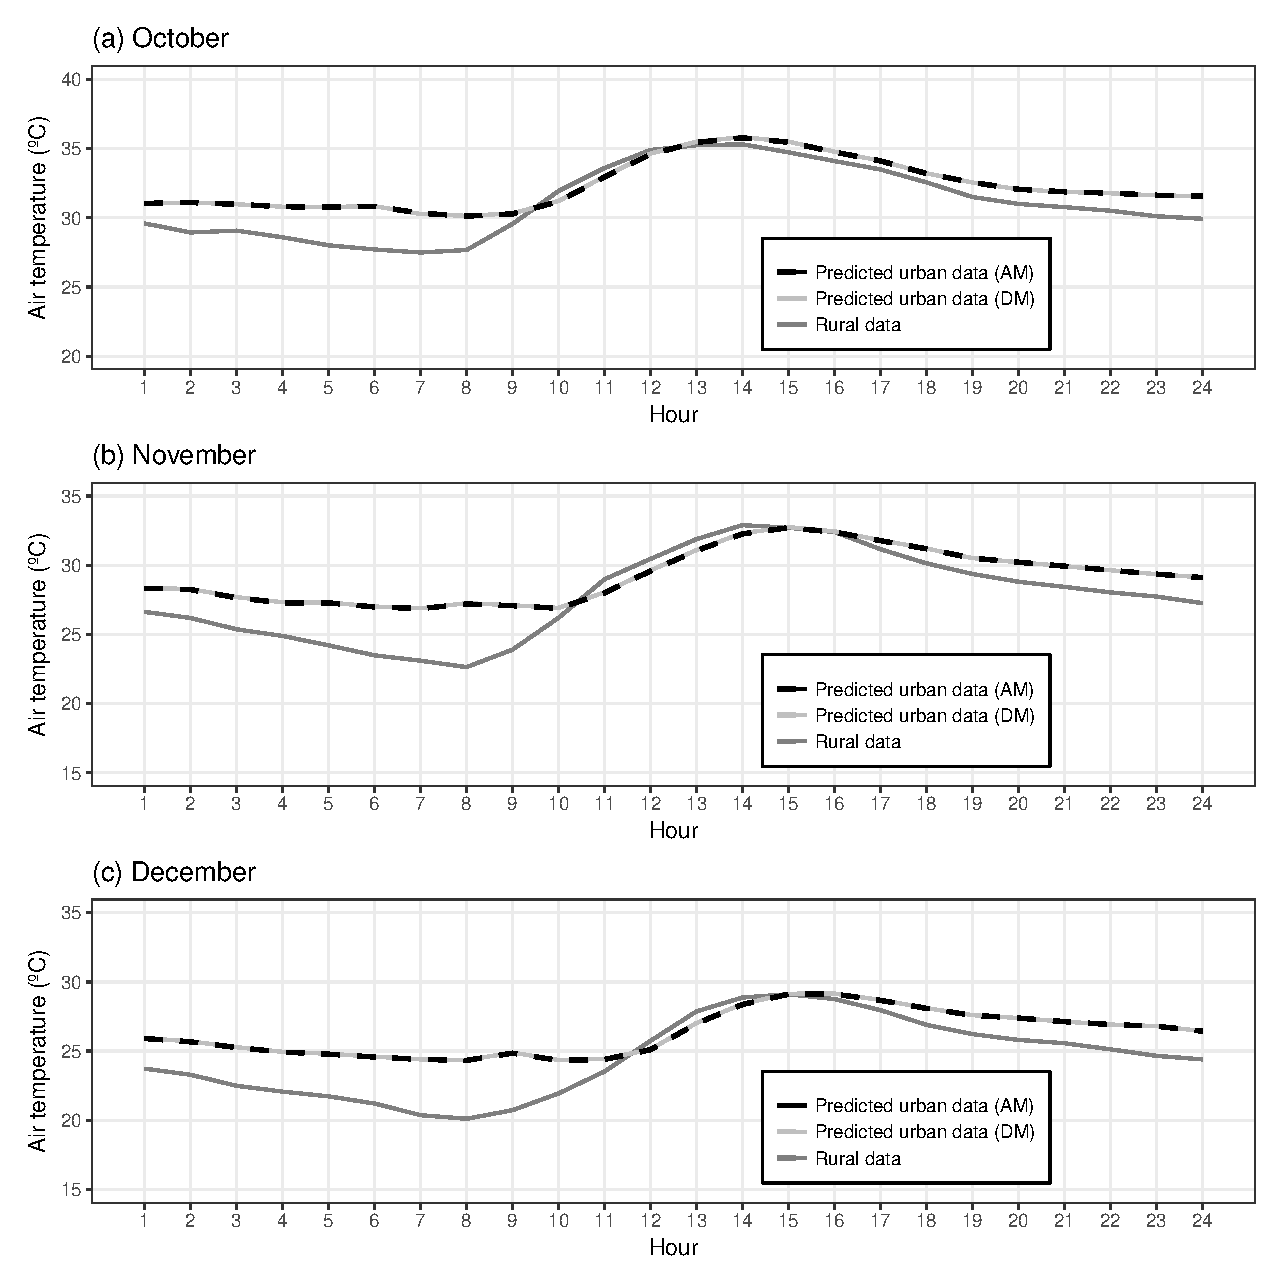
\includegraphics[width=.8\linewidth]{Figure3-4.eps}
\caption{Weekly-average diurnal profiles of the rural and urban outdoor air temperature: (a) Data between October 1 and 7, 2016; (b) Data between November 1 and 7, 2016; (c) Data between December 1 and 7, 2016.}
\end{figure}

We can also see that the DM and AM present almost the same profile of the urban outdoor air temperature. The differences in the diurnal pattern, computed as the root-mean-square error (RMSE) between the DM and AM, are all about 0.03 $^{\circ}$C from October to December. On the other hand, the difference in urban electricity use between the DM and AM can be observed to some extent in \textbf{Figure 3-5}, especially during the daytime. The corresponding diurnal differences, computed as the RMSE between the DM and AM, are respectively about 0.52, 0.59, and 0.64 MWh in October, November, and December. Usually there are more cooling demands during the daytime than during the nighttime for Abu Dhabi, resulting in more significant impacts of building-related parameters on the urban energy consumption. Nevertheless, the differences are not very high given the state of the art of urban energy modeling. This justifies the application of AM in the UWG to assess the aggregated effect of building energy models on the outdoor microclimate conditions in the subsequent uncertainty/sensitivity analysis and model calibration.

\begin{figure}
\centering
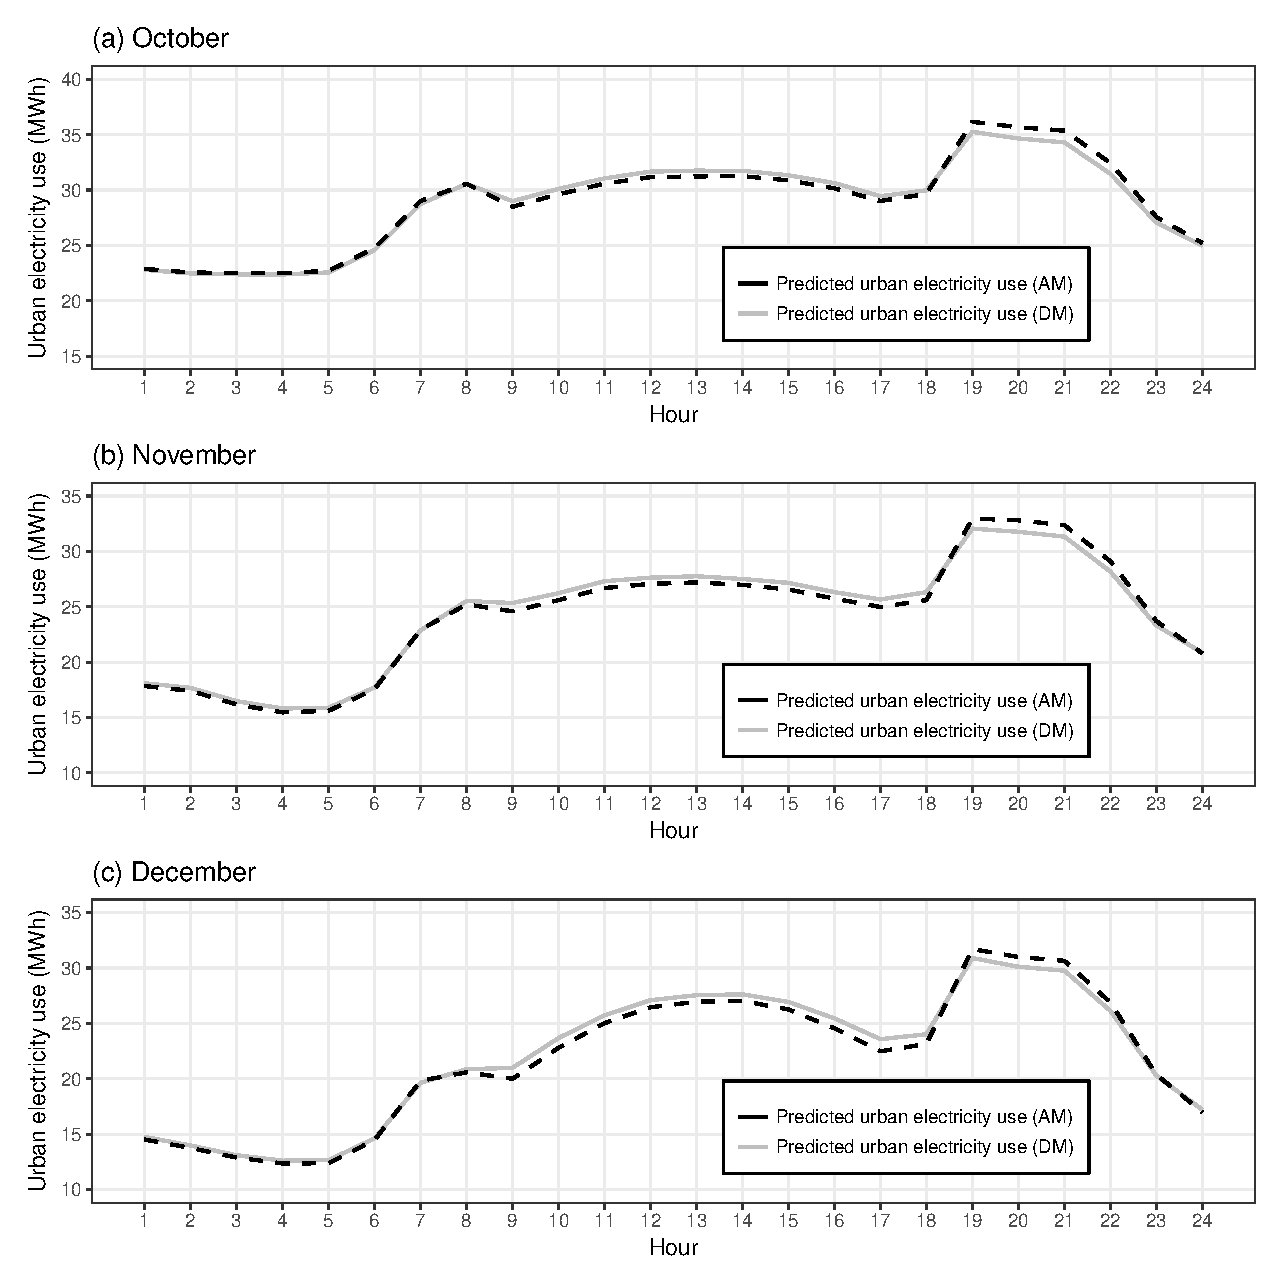
\includegraphics[width=.8\linewidth]{Figure3-5.eps}
\caption{Weekly-average diurnal profiles of the predicted urban electricity use: (a) Data between October 1 and 7, 2016; (b) Data between November 1 and 7, 2016; (c) Data between December 1 and 7, 2016.}
\end{figure}

The capacity of the UWG baseline model with the averaged building energy models to predict the urban outdoor air temperature is evaluated against the observations from October to December 2016, as shown in \textbf{Figure 3-6}. To properly describe the air temperature in the whole area of District E3 and to account for the sensor measurement uncertainty, we considered the average and standard deviation of the three sensors. \textbf{Figure 3-6} illustrates that the UWG tends to either over-predict or under-estimate the urban air temperature to some extent in the daytime. In general, the prediction performance is relatively better during the nighttime than during the daytime. Although validation of the electricity use prediction has not been performed -- due to our current inability to access such data -- we expect to obtain the corresponding meter data and will include such validation in the future. Still, considering the complexity of urban systems, the UWG can roughly capture the UHI pattern and produce some plausible values regarding the urban microclimate condition.

\begin{figure}
\centering
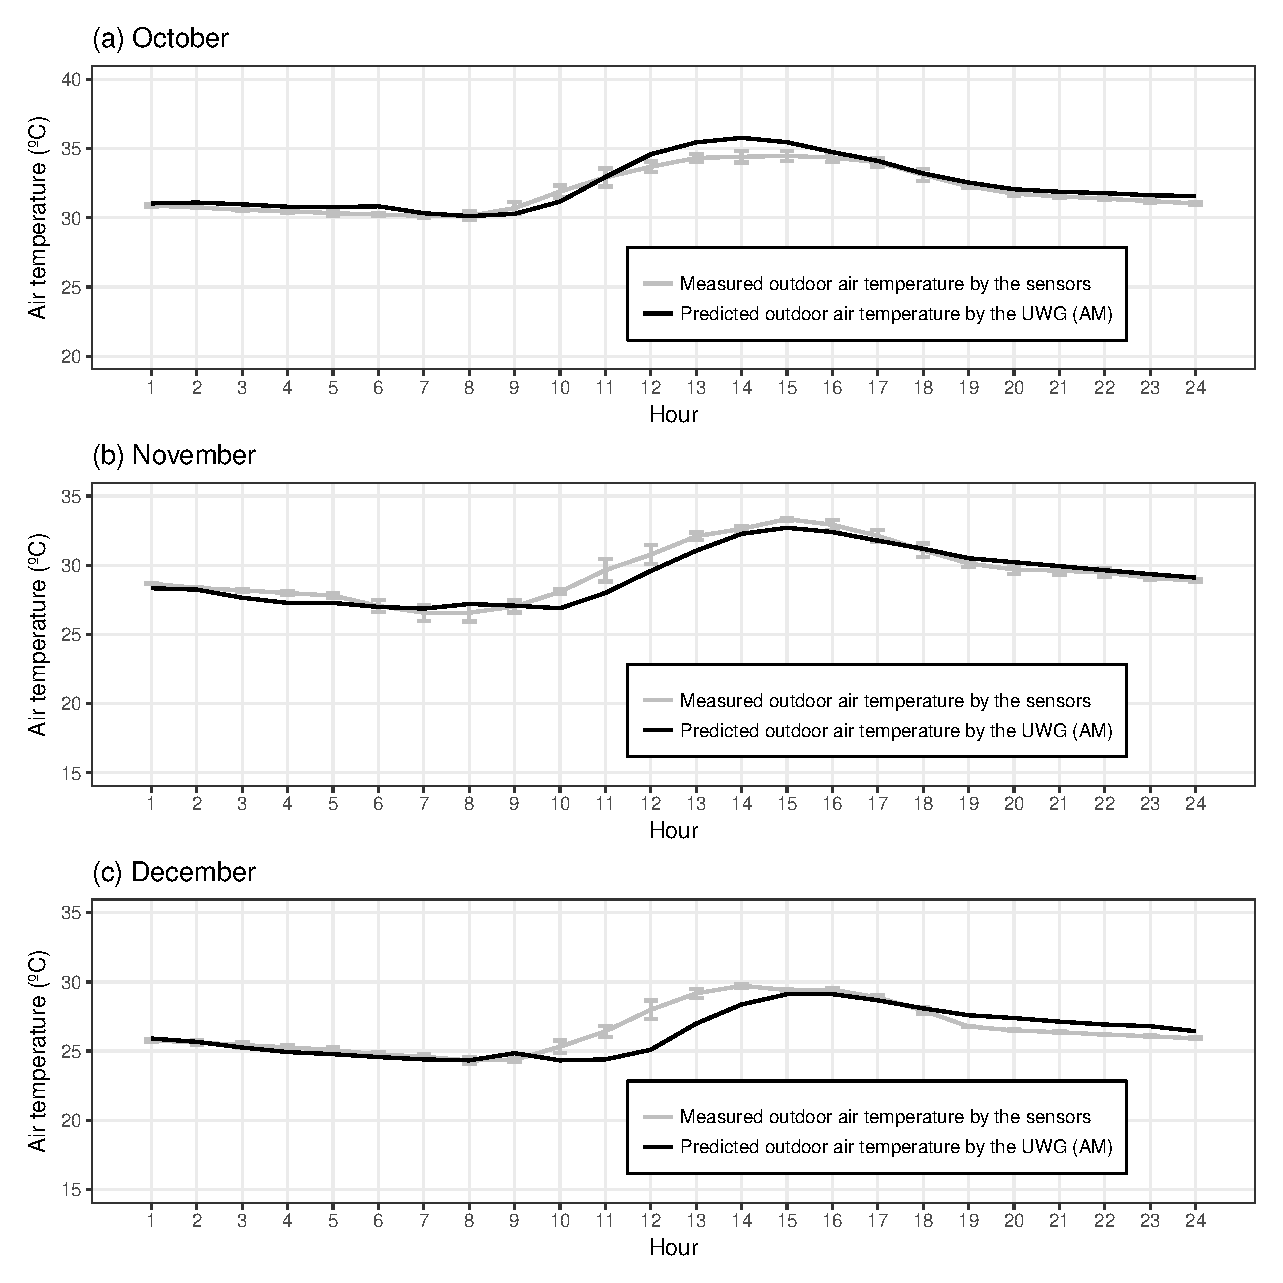
\includegraphics[width=.8\linewidth]{Figure3-6.eps}
\caption{Weekly-average diurnal profiles of the measured and predicted urban outdoor air temperature: (a) Data between October 1 and 7, 2016; (b) Data between November 1 and 7, 2016; (c) Data between December 1 and 7, 2016. The error bar represents the standard deviation of the measured urban outdoor air temperature from different sensors.}
\end{figure}

\chapter{Methodology}

\AddToShipoutPictureBG*{%
  \AtPageUpperLeft{%
    \hspace*{18.25cm}%
    \raisebox{-3cm}{%
      \makebox[0pt][r]{\parbox{\textwidth}{\begin{flushright}\textit{``Premature optimization is the root of all evil.''}\\
      Donald Knuth\end{flushright}}}
}}}%

The measurement uncertainty has been taken into account, but not the simulation uncertainty. The objectives of this chapter are to create a pool of candidate inputs with associated uncertainties, select the sensitivity analysis method to identify key system parameters, and develop the model calibration algorithm to auto-capture the system dynamics.

\section{Overview}

Model calibration is commonly regarded as an inverse estimation process where the selected input parameters are tuned to reconcile the outputs from simulation as closely as possible to the measurements. Generally there are three technical parts: model pre-establishment, model calibration, and model post-evaluation. In this study, the UWG is selected as the simulation engine to implement the calibration, since it can be applied to different climate zones and urban configurations to yield an estimation of the UHI effect to some extent.

\begin{figure}
\centering
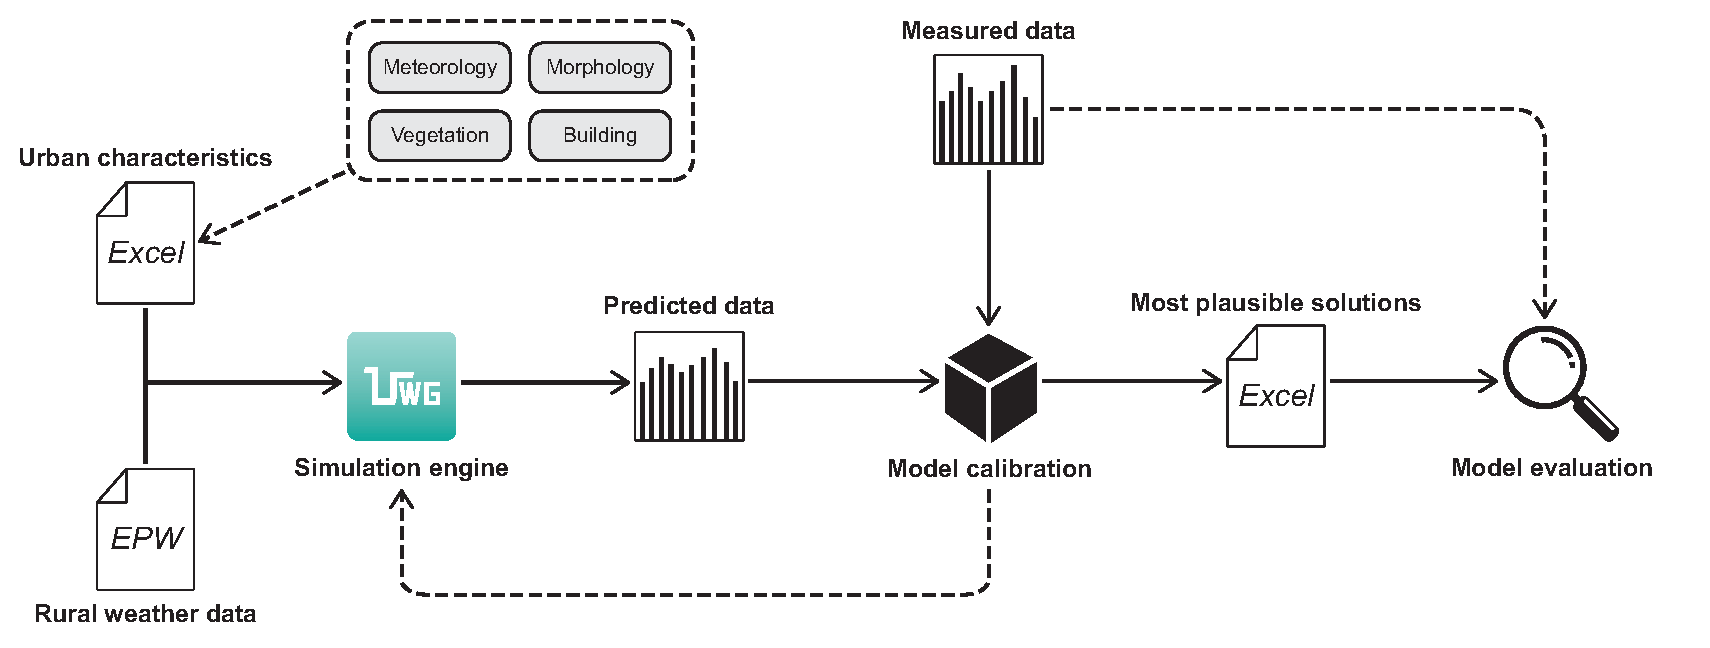
\includegraphics[width=.95\linewidth,trim=0 0 10 0,clip]{Figure4-1.eps}
\caption{General workflow of model calibration via the UWG.}
\end{figure}

As shown in \textbf{Figure 4-1}, the whole process starts by establishing case-specific UWG input files via the Excel interface facilitated by \textsc{Matlab}. Then, the simulated outputs are collected along with the measured data to initiate the calibration algorithm. Once the most plausible solutions are produced, they will be further examined to evaluate the system behavior.

The core methodology of calibrating a simulation program against the real data needs to be rational, robust, and efficient. Besides, it should have the flexibility for different users with different levels of preference and target. It is recognized from previous studies \cite{saltelli2002sensitivity,oliva2003model} that calibrating a detailed model with numerous parameters is a highly underdetermined problem, which may yield multiple non-unique solutions. The conventional wisdom is that once a model is calibrated in a certain sense, the effect of some intended adaption measures (i.e., parameter variations) could be assessed with a high level of confidence. This idea could be misleading since the urban microclimate condition is the aggregate behavior of many components in the system. Even if the optimization algorithm exhibits an overall good calibration performance, some of the individual parameters might be inaccurately identified. Therefore, it is unlikely that any one optimal solution can be deemed the ``best.'' Instead, we posit that it is more reasonable to identify the most plausible solutions (that are able to perform well under some specified measure) with associated uncertainties for a fairly robust calibration method.

Within this context, the calibration framework developed in this thesis generally enjoys the methodology proposed by Reddy et al. \cite{sun2006calibration,reddy2007calibrating}. The basic structure, shown in \textbf{Figure 4-2}, involves the following five steps:

\begin{figure}[h]
\centering
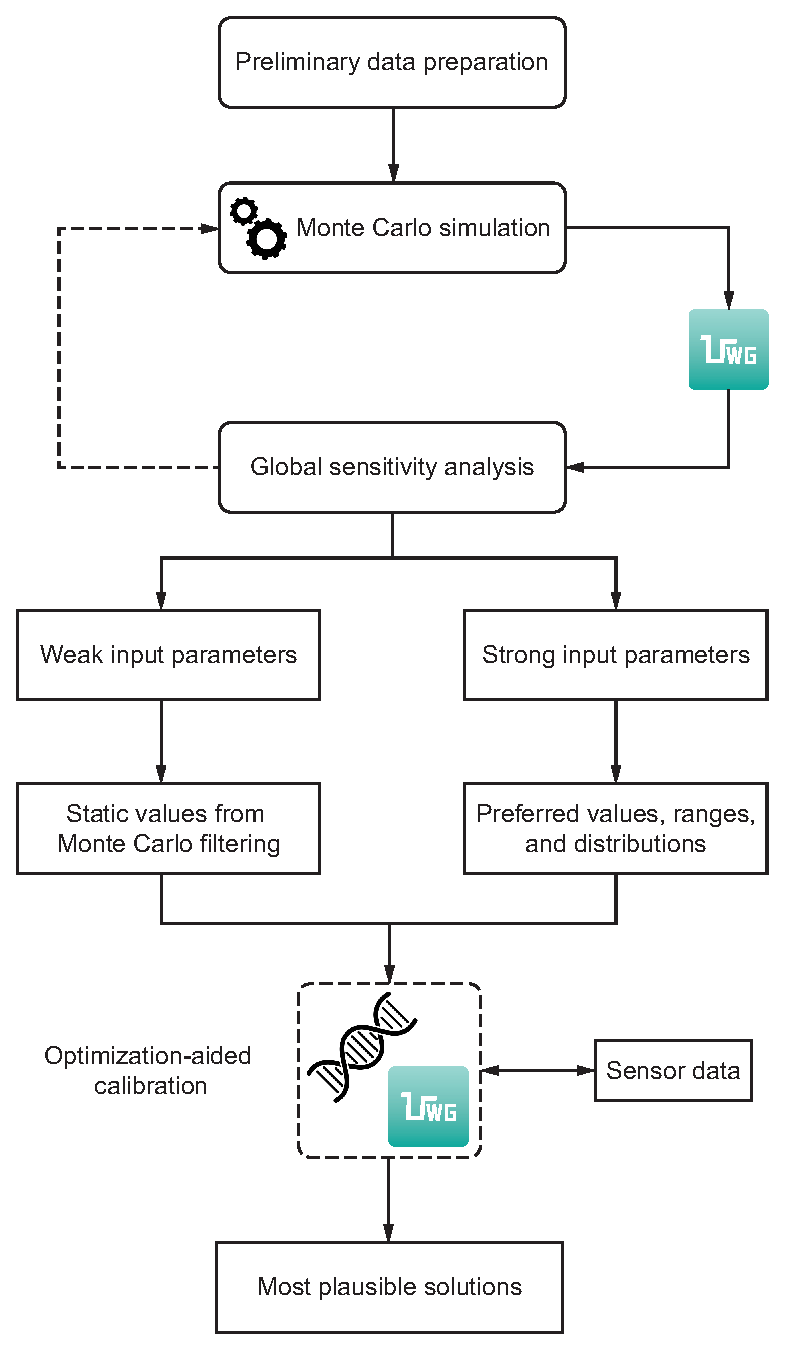
\includegraphics[width=.53\linewidth]{Figure4-2.eps}
\caption{Structure of an optimization-aided calibration method via the UWG.}
\end{figure}

\begin{enumerate}[\textit{Step} \itshape1:]
  \item Prepare the baseline information of the neighborhood area as precisely as possible. This enables the UWG to simulate the microclimate condition in the target street-level area.
  \item Identify a set of candidate parameters along with their preferred defaults and ranges. This provides some potential options for model calibration and adaption measures.
  \item Perform uncertainty and sensitivity analysis with different combinations of the inputs. This improves the understanding of the system by identifying the significant parameters.
  \item Apply guided search and optimization algorithm to refine the solutions automatically. This results in a set of plausible solutions that may represent the system dynamics.
  \item Evaluate the calibration effectiveness and efficiency of these solutions under uncertainty. This examines how likely the calibrated model is to yield biased system predictions.
\end{enumerate}

Since \textbf{Chapter 3} has detailed the baseline model of the present case study (\textit{Step 1}), the following subsections will further illustrate the technical guidelines and procedures of sensitivity/uncertainty analysis and model calibration (\textit{Steps 2-4}).

\section{Candidate input parameter}

Before conducting sensitivity/uncertainty analysis and model calibration, it is important to determine what input parameters with corresponding uncertainties are to be studied and what method is to be used. 

Defining a pool of candidate input parameters with reasonable uncertainties is often an arduous task which requires a sensible engineering judgment. Based on previous studies \cite{bueno2013urban,bueno2014computationally,bueno2013calculation} and local engineering practices \cite{martin2015estimation,deru2011us,radhi2009evaluating,afshari2014life}, 30 parameters are selected and categorized into four groups for the present study (see \textbf{Table 4.1}). For the parameters in the group of meteorological factors, urban characteristics, and vegetation variables, the uncertainty ranges are intentionally defined rather broadly in order to take all the possible uncertainties into account. In terms of most building-related parameters for a specific case study, values could be obtained within relatively small uncertainty ranges from available reports and technical specifications. The corresponding values of the remaining unselected parameters are taken as defaults from the data shown in \textbf{Tables 3.1 and 3.3}. Yet, disregarding uncertain input parameters can cause a fraction of the total output uncertainty to remain unexplained in the results, which should be considered in the interpretation of the outcomes.

Uncertainty can be generally classified as \textit{aleatory} and \textit{epistemic} uncertainty \cite{helton1996guest}. Aleatory uncertainty refers to the inherent randomness in the system behavior, while epistemic uncertainty comes from a lack of knowledge about the appropriate value in a specific application. The parameters associated with aleatory uncertainty are assumed to have a \textit{normal} distribution, which is suitable for measured physical properties. On the other hand, the parameters associated with epistemic uncertainty are approximated with a \textit{uniform} distribution, which represents that all the values are equally likely to happen. \textbf{Table 4.1} summarizes the distribution and uncertainty for each parameter.

\begin{table}[]
\footnotesize
\begin{center}
\caption{Uncertainty of the model parameters for District E3 in Abu Dhabi.}
\label{my-label}
\makebox[\linewidth]{
\begin{tabular}{lllll}
\toprule
No  & Parameter                                    & Unit        & Distribution & Uncertainty   \\ \hline
\multicolumn{5}{l}{\rule{0pt}{4ex}\textit{Meteorological factors}\vspace{6pt}}                                             \\
\hspace{6pt}A1  & Daytime urban boundary layer height          & m           & Uniform      & 500 -- 1000    \\
\hspace{6pt}A2  & Nighttime urban boundary layer height        & m           & Uniform      & 50 -- 100      \\
\hspace{6pt}A3  & Reference height of the VDM                  & m           & Uniform      & 100 -- 200     \\
\hspace{6pt}A4  & Circulation coefficient                      & -           & Uniform      & 0.8 -- 1.2     \\
\hspace{6pt}A5  & UCM-UBL exchange coefficient                 & -           & Uniform      & 0.1 -- 0.9     \\
\hspace{6pt}A6  & Heat flux threshold for daytime conditions   & W m$^{-2}$       & Uniform      & 150 -- 250     \\
\hspace{6pt}A7  & Heat flux threshold for nighttime conditions & W m$^{-2}$       & Uniform      & 40 -- 60  \vspace{6pt}     \\
\multicolumn{5}{l}{\textit{Urban characteristics}\vspace{6pt}}                                              \\
\hspace{6pt}B1  & Average building height                      & m           & Normal       & 35 $\pm$ 5        \\
\hspace{6pt}B2  & Fraction of waste heat into canyon           & -           & Uniform      & 0.1 -- 0.9     \\
\hspace{6pt}B3  & Building density                             & -           & Normal       & 0.25 $\pm$ 0.10   \\
\hspace{6pt}B4  & Vertical-to-horizontal ratio                 & -           & Normal       & 2.2 $\pm$ 0.5     \\
\hspace{6pt}B5  & Urban area characteristic length             & m           & Uniform      & 800 -- 1200    \\
\hspace{6pt}B6  & Road albedo                                  & -           & Normal       & 0.165 $\pm$ 0.080 \\
\hspace{6pt}B7  & Traffic sensible anthropogenic heat (peak)   & W m$^{-2}$       & Normal       & 20 $\pm$ 5   \vspace{6pt}     \\
\multicolumn{5}{l}{\textit{Vegetation variables}\vspace{6pt}}                                               \\
\hspace{6pt}C1  & Urban grass coverage                         & -           & Uniform      & 0 -- 0.1       \\
\hspace{6pt}C2  & Urban tree coverage                          & -           & Uniform      & 0 -- 0.1       \\
\hspace{6pt}C3  & Vegetation albedo                            & -           & Normal       & 0.25 $\pm$ 0.05   \\
\hspace{6pt}C4  & Latent fraction of grass                     & -           & Uniform      & 0.45 -- 0.75   \\
\hspace{6pt}C5  & Latent fraction of tree                      & -           & Uniform      & 0.5 -- 0.9     \\
\hspace{6pt}C6  & Rural vegetation coverage                    & -           & Uniform      & 0 -- 0.1  \vspace{6pt}     \\
\multicolumn{5}{l}{\textit{Building systems}\vspace{6pt}}                                                   \\
\hspace{6pt}D1  & Glazing ratio                                & -           & Normal       & 0.5 $\pm$ 0.15    \\
\hspace{6pt}D2  & Wall U-value                                 & W m$^{-2}$ K$^{-1}$   & Normal       & 2.5 $\pm$ 1       \\
\hspace{6pt}D3  & Window U-value                               & W m$^{-2}$ K$^{-1}$   & Normal       & 3.25 $\pm$ 1      \\
\hspace{6pt}D4  & Window SHGC                                  & -           & Normal       & 0.60 $\pm$ 0.15   \\
\hspace{6pt}D5  & Infiltration rate                            & ACH         & Uniform      & 0.1 -- 0.7     \\
\hspace{6pt}D6  & Chiller COP                                  & -           & Uniform      & 2 -- 4         \\
\hspace{6pt}D7  & Indoor air temperature set point             & $^{\circ}$C          & Uniform      & 20 -- 24       \\
\hspace{6pt}D8  & Equipment load density                       & W m$^{-2}$       & Normal       & 13 $\pm$ 3        \\
\hspace{6pt}D9  & Lighting load density                        & W m$^{-2}$       & Normal       & 10 $\pm$ 3        \\
\hspace{6pt}D10 & Occupancy density                            & m$^2$ person$^{-1}$ & Uniform      & 15 -- 25       \\
\bottomrule
\end{tabular}
}
\end{center}
Note: \\
(a) For the input parameter assumed to have a normal distribution, the uncertainty is represented as ($\mu \pm 3\sigma$), where $\mu$ is the mean and $\sigma$ is the standard deviation of the distribution. \\
(b) The parameter uncertainty is mainly assigned based on the data taken from the local building design/energy codes provided by the Abu Dhabi Municipality (via personal contact), the prevailing engineering practices \cite{martin2015estimation,deru2011us,radhi2009evaluating,afshari2014life}, and the previous investigations \cite{bueno2013urban,bueno2014computationally,bueno2013calculation}. \\
(c) The physical properties of some parameters (e.g., B6 and C3) are considered according to the work by Stewart and Oke \cite{stewart2012local}. \\
(d) Detailed physical definition of the parameters can be found in Refs. \cite{bueno2013urban,bueno2013calculation}. In particular, Ref. \cite{bueno2013urban} illustrates the parameters in the RSM and UC-BEM, while Ref. \cite{bueno2013calculation} illustrates the parameters in the VDM and UBLM.

\end{table}

\section{Global sensitivity analysis}

The next step is to design and implement a global sensitivity analysis (SA) to find the most influential parameters and to evaluate the effects of their uncertainties on the predicted urban microclimatic performance for different seasons in Abu Dhabi. Selecting analysis methods with suitable sensitivity indices usually relies on a good mathematical understanding of the engineering systems.

\subsection{Regression-based analysis}

Commonly used global SA methods in simulations include screening-based, regression-based, and variance-based methods. The technical details of these methods can be found in Refs. \cite{saltelli2004sensitivity,helton2006survey,storlie2009implementation}. The selection of the SA method for a specific case study depends on many factors, such as the research purpose, the number of input parameters, the potential computational cost, etc. In particular, the regression analysis based on Monte Carlo sampling is regarded as a good practice in the global SA of built environments \cite{de2009identification,eisenhower2012uncertainty,nguyen2015performance,menberg2016sensitivity}. This is because the quasi-random sampling techniques can potentially offer more detailed quantitative insights into the system behavior with moderate computational costs.

As a pilot, the present study performs a global regression-based SA using the random sampling method. Technically speaking, a Monte Carlo SA provides statistical outcomes to a problem by running multiple models with a probabilistically generated input sample. These simulated results are then used to quantify the output uncertainty and calculate the sensitivity indices. As recommended by Tian \cite{tian2013review}, we implement the \textsc{SimLab} \cite{simlab2} to automate the sampling work and use the \textsc{R} program \cite{pujolglobal} to conduct the uncertainty/sensitivity analysis. It is important to note that the Latin Hypercube (LH) sampling strategy is applied in this study due to its efficient stratification properties \cite{helton2006survey}.

\begin{figure}[!b]
\centering
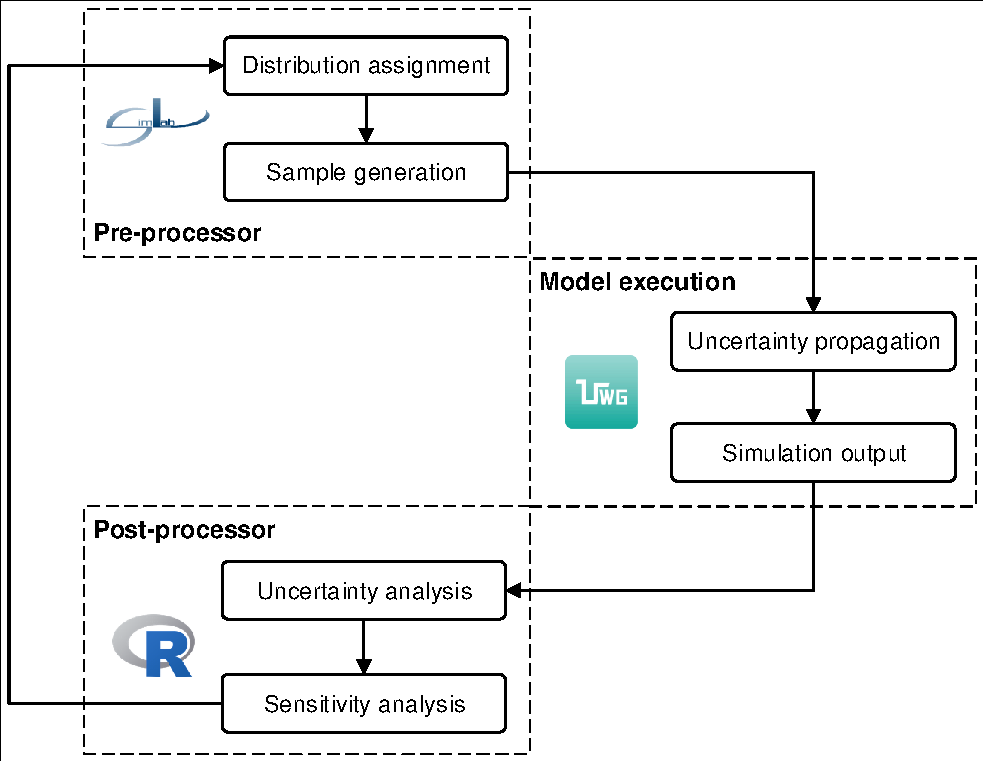
\includegraphics[width=.55\linewidth,trim=2 2 2 2,clip]{Framework.pdf}
\caption{General process of a global regression-based analysis using the \textsc{SimLab}, UWG, and \textsc{R} program.}
\end{figure}

The general analysis process is structured as shown in \textbf{Figure 4-3}. It starts by defining the distributions for aleatory and epistemic uncertainty and by producing the input samples automated via \textsc{SimLab}. Then, the sample data is read to create UWG input files via the Excel interface facilitated by \textsc{Matlab}. In the meantime, the \textsc{Matlab} code checks whether any severe or fatal errors occur during the parametric simulations. Finally, the outputs are collected to quantify the uncertainty/sensitivity indices, which is supported by the \textsc{R} sensitivity package. In the present study, effects due to the correlation between various inputs are assumed to be negligible.

The number of parametric simulations (sample size) for a reliable Monte Carlo analysis should be large enough to ensure convergence of the sensitivity indices but not be so large as to delay the SA process. For the regression-based analysis, although nearly no formal explanation has been presented, Saltelli et al. \cite{saltelli2004sensitivity} recommended the sample size of 1.5 -- 10 times the number of input parameters. Some researchers \cite{nguyen2015performance,menberg2016sensitivity} examined the convergence behavior with various simulation runs but gave quite different conclusions about the appropriate value. From the available experience and references, we choose to execute 1000 simulation runs for the summer and winter cases, respectively. This choice is a compromise between analysis accuracy and computational cost.

\subsection{Sensitivity index}

To estimate the sensitivity indices using the regression-based method, the model response is approximated by a multidimensional polynomial equation with a regression coefficient for each input. Then, the estimated regression coefficients are standardized using the variance of the corresponding input parameter and the variance of the model response \cite{saltelli2004sensitivity}. If a first-order polynomial is chosen, we will obtain the so-called standardized regression coefficient (SRC). The absolute value of the SRC represents a measure of parameter importance, with higher SRCs indicating more impact on the model output. In addition, the sign of the SRC shows whether the model output will increase or decrease as the corresponding input changes.

Many researchers \cite{tian2013review} have applied the sensitivity indices based on the rank transformation (SRRC) to investigate non-linear but monotonic models. However, the rank transformation techniques would change the model during the calculation, thereby leading to the sensitivity information of a different model \cite{saltelli2004sensitivity}. Such transformation would make the convergence of the sensitivity indices more difficult \cite{nguyen2015performance} and result in unstable outcomes. In addition, the available references indicate that the SRRC did not exhibit any outstanding performance \cite{de2009identification,nguyen2015performance}, while the SRC could keep quite stable and in good agreement with the indices from more sophisticated global SA methods \cite{menberg2016sensitivity}. Thus, the SRC is used in the present study to interpret a quantitative measure for the influence of the inputs on the model outputs.

However, the feasibility of the SRC is limited to the model responses that can be sufficiently approximated by the fitted regression model. The SRC is not reliable when the model under investigation is highly non-linear. In order to measure how well the regression model fits the model output, we use the coefficient of determination (R$^2$). Ranging from zero to one, the coefficient of determination tests how much the variance of the model response is explained by the variance of the regression model. The larger the R$^2$ is, the better the model will fit the data. Saltelli et al. \cite{saltelli2004sensitivity} have recommended a threshold of R$^2$ = 0.7 for a fairly strong regression model and its resulting SRCs.

\section{Model calibration}
 After the global SA is performed, the non-influential parameters will be fixed at some nominal values while the influential parameters will be further refined automatically via search and optimization algorithms. In particular, the Monte Carlo filtering technique and online hyper-heuristic evolutionary algorithm are proposed and developed in the present study. 

\subsection{Objective function}

Goodness-of-fit (GOF) is an index that relates the dispersion between the measured and simulated data via a statistical model. Many researchers \cite{ruiz2017analysis,reddy2007calibrating} have recommended and adopted the GOF as the objective for model calibration. Lower values mean that the model is more accurate and its behavior fits better with the real case. The GOF is defined as:

\begin{equation}
\textrm{GOF} = \sqrt{\frac{w^2_{\textrm{NMBE}} \textrm{NMBE}^2 + w^2_{\textrm{CV(RMSE)}} \textrm{CV(RMSE)}^2}{w^2_{\textrm{NMBE}} + w^2_{\textrm{CV(RMSE)}}}}\,,
\end{equation}
\vspace{12pt}
\noindent where
\vspace{0em}
\begin{equation}
\textrm{NMBE} = \frac{1}{\bar{m}} \frac{\sum_{i=1}^n (s_i - m_i)}{n}\,,
\end{equation}

\begin{equation}
\textrm{CV(RMSE)} = \frac{1}{\bar{m}} \sqrt{\frac{\sum_{i=1}^n (s_i - m_i)^2}{n-1}}\,.
\end{equation}

\vspace{15pt}
The NMBE (normalized mean bias error) quantifies the relative error of the simulated values with respect to the measured values summed over the selected number of time steps. Positive values indicate that the model over-estimates the actual scenarios, while the under-prediction produces negative values. As a counterpart, the CV(RMSE) (coefficient of variation of the root-mean-square error) indicates the variability of the errors (i.e., uncertainty) between the simulated ($s_i$) and measured ($m_i$) data. For numerical stability during optimization, $\bar{m}$ is set as the mean of the absolute values.

If the simulation results are plotted on an $x$-$y$ plane with NMBE and CV(RMSE) as the axes, one would like to identify a set of trade-off optimal solutions (i.e., a Pareto set) as the ``better'' solution set. This method is referred to as ``multi-objective optimization'' or ``Pareto optimization.'' For any given problem, the Pareto optimal set can be produced by an infinite number of Pareto points. A potential drawback of this approach is slower algorithm convergence and hence lower computational efficiency, compared with the performance of single-objective optimization \cite{ruiz2017analysis}. In addition, the problem of how to select the best solution from the Pareto set is not trivial since it depends on many aspects \cite{nguyen2014review}.

To avoid multi-objective optimization in the present case study, we use the idea of ``scalarization.'' Different weights are assigned to each index, and then the multi-objective function will be simplified as a weighted function of the criteria. Accordingly, we introduce a set of weights, $w_{\textrm{NMBE}}$ and $w_{\textrm{CV(RMSE)}}$, to impact our consolidated indices in Equation (4.1), where $w_{\textrm{NMBE}} + w_{\textrm{CV(RMSE)}} = 1$. Thus, the estimation of a Pareto front can be achieved by running single-objective optimizations with various weights.

In practice, energy and environment researchers would prefer the model to capture the bias (i.e., NMBE) more precisely than the variation (i.e., CV(RMSE)). This argument has been supported by the ASHRAE Guideline 14-2002 (RP-1051) \cite{reddy2007calibrating,guideline2002guideline}, which recommends a ratio of 3: 1 for $w_{\textrm{NMBE}}$: $w_{\textrm{CV(RMSE)}}$. Therefore, in the present study, we adopt this rule and set the $w_{\textrm{NMBE}}$ and $w_{\textrm{CV(RMSE)}}$ to be 0.75 and 0.25, respectively.

\subsection{Monte Carlo filtering}

Before conducting a fine calibration, it is important to reduce the dimensionality of the parameter space by identifying strong and weak parameters among the set of candidate inputs. Another intent is to detect the local ranges most likely to contain the ``actual'' value for each parameter. This can be achieved by adopting a blind Monte Carlo (MC) search coupled with sensitivity analysis (SA). In general, MC filtering is a process of rejecting sets of model outputs that are far from reality, while the SA can produce an influential parameter set that meets some prescribed criteria. Once the strong parameters are determined, the weak parameters can be fixed at some nominal values.

We have illustrated the details of regression-based SA through MC sampling in \textbf{Subsection 4.3}. After an LHMC batch run and regression-based analysis are completed, the strong parameters can be identified and the GOF indices can be computed for each trial. Those input vectors that result in unfavorable GOF values will be ruled out. On the other hand, the information contained in the ``good'' input vectors can be used to set values for the weak parameters, which can then be removed from further consideration in the calibration process. In particular, we use the average values of these promising input vectors to fix the weak parameters.

Once the MC filtering has identified a set of strong parameters, we can use the information advantageously to further fine-tune these influential inputs via heuristic-based search methods such as the evolutionary algorithm.

\subsection{Online hyper-heuristic evolutionary algorithm}

Evolutionary algorithms (EAs) have been widely used in a variety of complex real-world applications. However, EAs need to perform a large number of fitness (or objective) function evaluations in order to get optimal or near-optimal solutions. For engineering problems, each fitness function is evaluated via physics-based simulation, which often makes the whole process computationally expensive. Hyper-heuristics represent a class of methods that could address this barrier and reduce computational cost.

A hyper-heuristic search method seeks to automate, often by incorporation of statistical or machine learning techniques, the process of handling several simpler heuristics to efficiently solve computational search problems. The overall goal is to reduce the number of numerical simulations along a search path at the algorithm level. One popular paradigm is to construct a so-called surrogate or meta-model that can approximate the behavior of the original fitness function in the optimization process. The idea of hyper-heuristics can be traced back to the 1960s \cite{dunham1963design}, while managing approximate models in optimization via EAs has received continuous attention since the 1990s \cite{jin2005comprehensive}.

Based on how the surrogate models are used during the evolution, the hyper-heuristics can be further classified as \textit{offline} and \textit{online}. Offline hyper-heuristics utilize a surrogate model that is trained in advance, separately from the evolution process. This needs to be pre-validated and the surrogate must be updated to support a new case study. In online hyper-heuristics, a surrogate model is continuously retrained during the evolution and thus can make use of the most recent data. The self-updating mechanism without any pre-simulated database enables the online method to flexibly allow for many ``plug-and-play'' applications. Therefore, online hyper-heuristics have been very popular in engineering optimization problems \cite{tenne2010computational}.

\begin{table}[h]
\footnotesize
\begin{center}
\caption{Hyper-parameters of the evolutionary algorithm and support vector regression used in the model calibration.}
\label{my-label}
\begin{tabular}{ll}
\toprule
Hyper-parameter                         & Setting                        \\ \hline
\rule{0pt}{4ex}\textit{Evolutionary algorithm}\vspace{6pt}         &                                \\
\hspace{9pt}Algorithm type                          & Evolutionary strategy          \\
\hspace{9pt}Objective function                      & Goodness-of-fit                \\
\hspace{9pt}Parent population size $|P|$              & 120                            \\
\hspace{9pt}Offspring population size $|Q|$           & 120                            \\
\hspace{9pt}Surrogate population size $|S|$           & 360                            \\
\hspace{9pt}Maximum number of generations           & 60                             \\
\hspace{9pt}Maximum number of expensive evaluations & 2040                           \\
\hspace{9pt}Crossover algorithm                     & Laplace                        \\
\hspace{9pt}Crossover probability                   & 0.8                            \\
\hspace{9pt}Mutation algorithm                      & Power                          \\
\hspace{9pt}Mutation probability                    & 0.005                          \\
\hspace{9pt}Proportion of elitism                   & 0.2       \vspace{6pt}                    \\
\textit{Support vector regression}\vspace{6pt}      &                                \\
\hspace{9pt}Regression type                         & $\epsilon$-SV regression                \\
\hspace{9pt}Kernel function                         & Gaussian radial basis function \\
\hspace{9pt}Optimization method                     & Grid search                    \\
\hspace{9pt}Cross-validation                        & 5 folds                       
 \\
\bottomrule
\end{tabular}
\end{center}
Note: The hyper-parameters are set based on the prevailing engineering practices, previous related studies \cite{jin2005comprehensive,tenne2010computational,brownlee2015constrained,jin2011surrogate,deep2009real}, and trial and error. In particular, the surrogate population size is set to be three times of the parent population size \cite{brownlee2015constrained}, while the parent population size is set to be 10 times of the number of design parameters for single-objective optimization \cite{deep2009real}. The settings for the crossover and mutation operator follow the suggestions in Ref. \cite{deep2009real}. 
\end{table}

Although many researchers have utilized offline hyper-heuristics to calibrate the building energy models \cite{o2013leveraging,manfren2013calibration}, little is known to the author about the use of online hyper-heuristics. Very recently, some studies have been published to develop the online hyper-heuristic EAs for simulation-based multi-objective optimization in building design \cite{brownlee2015constrained,xu2016improving}. Therefore, we opt to embrace the methodology proposed by Brownlee and Wright \cite{brownlee2015constrained} and develop an online hyper-heuristic EA to calibrate an urban microclimate model. There are many possible ways to implement the general idea of online hyper-heuristics. The aim of this thesis is not to explore this whole space but simply to illustrate that one fairly straightforward application works well and that online surrogate model helps. As an illustrative example, the evolutionary strategy (ES) \cite{hansen1996adapting} in the \textsc{Matlab} environment and the support vector regression (SVR) \cite{cortes1995support} from LIBSVM \cite{chang2011libsvm} are selected for the present study due to their wide applications. \textbf{Table 4.2} summarizes the associated hyper-parameters. Although the convergence behavior of EA could be significantly affected by the hyper-parameters \cite{alajmi2014selecting}, we do not intend to explore this topic here and merely adopt some common settings.

\begin{figure}[h]
\centering
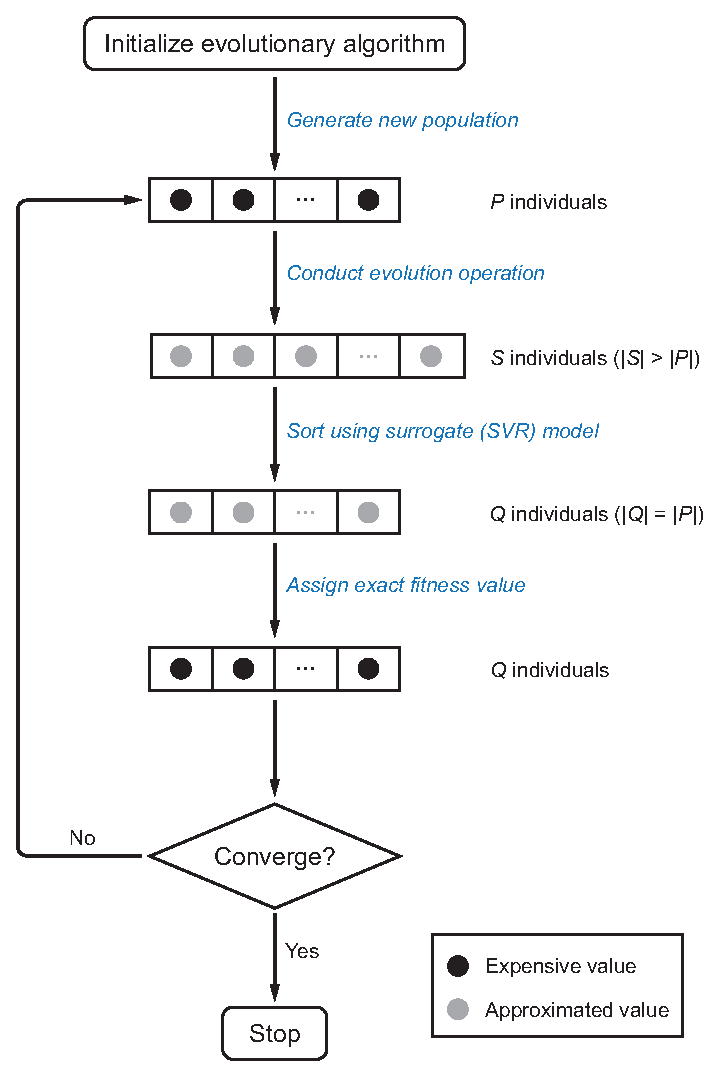
\includegraphics[width=.485\linewidth]{Figure4-3.eps}
\caption{General flowchart of an online hyper-heuristic EA (mainly from Ref. \cite{jin2011surrogate}).}
\end{figure}

\textbf{Figure 4-4} shows the procedure of an individual-based model management strategy, as described in Ref. \cite{jin2011surrogate}. In each generation, a local surrogate (SVR) model is trained if necessary. The role of SVR is to approximately evaluate the offspring in each generation and identify the most promising individuals among them, which will then be evaluated via expensive simulation. The latter are, of course, recorded and can be exploited as training patterns in the forthcoming generations. It is important to note that the surrogate model is \textit{not} used directly to examine the convergence behavior.

The pseudo-code of the proposed online hyper-heuristic EA for single-objective optimization is shown in \textbf{Algorithm 1}. The blue part (Steps 5-14) illustrates where and how a local surrogate model is built within the EA. At generation $t$, a surrogate (SVR) model needs to be updated if its accuracy is not acceptable. The SVR model is trained using the database $D$ that consists of previous population(s) $P$ and their expensive evaluations $F_{E,P}$ (Steps 5-10). Then, the crossover and mutation operators are used to generate a surrogate population $S$ (with size $|S| > |P|$) (Step 11). The SVR approximates the objective values in $S$ (Step 12), and the ES ranks $S$ (Step 13) with the highest ranking solutions inserted into the offspring population $Q$ (with size $|Q| = |P|$) (Step 14). $Q$ are then evaluated using the expensive UWG simulations, which will be appended into the database $D$ if they are not in $D$ before. Finally, the offspring $Q$ are assigned to be the parent $P$ in the next generation.

\begin{algorithm}[t]
\footnotesize
\caption{\textsc{Online Hyper-Heuristic Evolutionary Algorithm}}
\begin{algorithmic}[1]
\State initialize($P_t$) at $t$ = 1\Comment{Initialize new population}
\State $F_{E,P_t} = \textrm{obj-and-const-calc(} P_{t} \textrm{)}$\Comment{Expensive objective and constraint in $P$}
\State $D$ = cache($P_t$, $F_{E,P_t}$)\Comment{Store training data $P$ and $F$ into $D$}
\State \textbf{while} \textrm{not terminated} \textbf{do}
\color{blue}
\State \qquad \textbf{for all} \textrm{objective and constraint} \textbf{do}
\State \qquad\qquad \textrm{compute FPC in $P_{t}$}\Comment{Surrogate model performance}
\State \qquad\qquad \textbf{if} \textrm{FPC $<$ 0.7} \textbf{then}
\State \qquad\qquad \qquad \textrm{update-model($D$)}\Comment{Retrain model within the current generation}
\State \qquad\qquad \textbf{end if}
\State \qquad\textbf{end for}

\State \qquad $S = \textrm{make-new-pop(} P_{t} \textrm{)}$\Comment{Create surrogate population $S$ (with size $|S| > |P|$)}

\State \qquad $F_S = \textrm{obj-and-const-approx(} S \textrm{)}$\Comment{Approximated objective and constraint in $S$}

\State \qquad $S$ = rank($F_S, S$) \Comment{Rank individuals based on fitness values}

\State \qquad $Q_t$ = extract($S$) \Comment{Pre-select $Q$ individuals (with size $|Q| = |P|$)}
\color{black}

\State \qquad $F_{E,Q_t}$ = obj-and-const-calc($Q_t$) \Comment{Expensive objective and constraint in $Q$}

\State \qquad $D = D \cup (Q_t, F_{E,Q_t})$ \Comment{Add expensive evaluations into $D$}

\State \qquad $P_{t+1} = Q_t$ \Comment{Assign $Q$ as the next generation}

\State \qquad $t = t+1$\Comment{Increase generation counter}

\State \textbf{end while}

\end{algorithmic}
\end{algorithm}

The whole process continues until the evolution meets a stop criterion, e.g., the search exceeds the maximum number of generations or the maximum number of expensive simulations. In addition, we use a fitness prediction correlation (FPC) to measure the surrogate model accuracy. Usually the FPC is the Spearman's rank correlation, between the exact and approximated values, for one solution set. The threshold FPC for retraining is set as 0.7 \cite{brownlee2015constrained} for the present case study.
\chapter{Result and discussion}

\AddToShipoutPictureBG*{%
  \AtPageUpperLeft{%
    \hspace*{18.25cm}%
    \raisebox{-3cm}{%
      \makebox[0pt][r]{\parbox{\textwidth}{\begin{flushright}\textit{``The distance between insanity and genius is measured only by success.''}\\
      Bruce Feirstein\end{flushright}}}
}}}%

We have applied the proposed methods to an urban microclimate system simulated by the UWG. In particular, the UWG model has been calibrated based on the urban outdoor air temperature in District E3 of downtown Abu Dhabi (UAE) during 2017. This chapter presents and discusses the main results.

\section{Overview}

The case study was conducted in District E3, the same area detailed in \textbf{Chapter 3}. The measured rural data from the Masdar Institute Field Station during calendar year 2017 is used for running the UWG. For the urban outdoor air temperature, we use the data measured in 2017 from all six of the same calibrated sensors that present consistent performances. The locations of these sensors are depicted as the red-cross points in \textbf{Figure 3-1(c)}. The temperature observations at 8.5 m were selected for validating the calibrated models.

In this study, we use the urban-rural outdoor air temperature difference to cali-brate the UWG. A good fit between the predicted and measured temperature trajectories is one indication that the model has captured the thermal dynamics well. Other calibration studies based on energy use instead of air temperature may increase the solution uncertainty, since various combinations of the system properties can easily produce similar consumptions. We also find that some researchers have used air temperature to analyze or calibrate building thermal simulations \cite{ruiz2016genetic,ruiz2017analysis,spitz2012practical,cornaro2015thermal}.

First, a Latin Hypercube sample matrix of size $N = 1000$ has been generated and propagated via the UWG for summer (August 1-7) and winter (February 1-7) in 2017, respectively. For each trial, the predicted hourly outdoor air temperatures were saved. The computation of a one-week scenario lasted around \textit{one minute} on a 3.00GHz processor computer for each trial. To the author's knowledge, this is to date the fastest simulation engine to estimate the microclimate conditions for a specific urban site using physics-based model setting. Finally, corresponding indices (i.e., SRC and R$^2$) were calculated based on the generated results to enable uncertainty and sensitivity analysis.

Once the weak parameters were identified according to some specified criteria, their values were set via MC filtering based on the information contained in those input vectors with the lowest GOFs. The strong parameters, on the other hand, were considered to be tuned in the subsequent EA-based optimization. The objective function used to guide the EA is the GOF based on weekly-average diurnal profiles of the urban-rural outdoor air temperature difference in February 1-7 and August 1-7, 2017. That is, we are calibrating the strong parameters only based on the measurements in one summer week and one winter week.

In order to evaluate the associated uncertainty as predicted by the calibrated solutions, we ran 10 independent trials for both the traditional and online hyper-heuristic EAs. All the trials used the same stop criteria: the evolution ends when the number of expensive evaluations exceeds the maximum 2040 or the evolution lasts more than 60 generations. The goal is to find the algorithm setup returning the lowest GOF for the same number of evaluations within fixed computation budgets (i.e., better quality solution given the same effort); this goal precluded use of a convergence criterion. Also provided were comparisons of the computational effort required to obtain the same quality of solutions. An internal cache of previously-evaluated solutions is maintained in the online hyper-heuristic EA for each run, to avoid re-evaluating the same solutions. The solutions drawn from the cache do not count toward the limit of 2040. Finally, the resulting solution sets from the 10 trials of the online hyper-heuristic EA were evaluated using the measurements.

\section{Uncertainty analysis}

The cumulative distribution functions are used to present the results from the Monte Carlo simulations and to display percentiles and confidence intervals of the outputs. \textbf{Figure 5-1} illustrates the uncertainty range of the weekly-average diurnal profile of the predicted outdoor air temperature in summer and winter, 2017. The shaded area represents the predicted values ranging from the 5th to 95th percentile, while the solid line represents the predicted value of the 50th percentile (i.e., median). It can be said that a model is robust enough to simulate the underlying phenomenon if, fed by the inputs with a given uncertainty, it is able to produce responses in a suitably small range. Thus, we can claim from \textbf{Figure 5-1} that the UWG is a fairly good simulator to approximate the thermal behavior of an urban microclimate system for different seasons with a specific degree of robustness. In addition, the results are quite consistent with those in our former study \cite{mao2017global} when we performed identical analysis on the same UWG model for summer and winter in 2016.

\begin{figure}[]
\centering
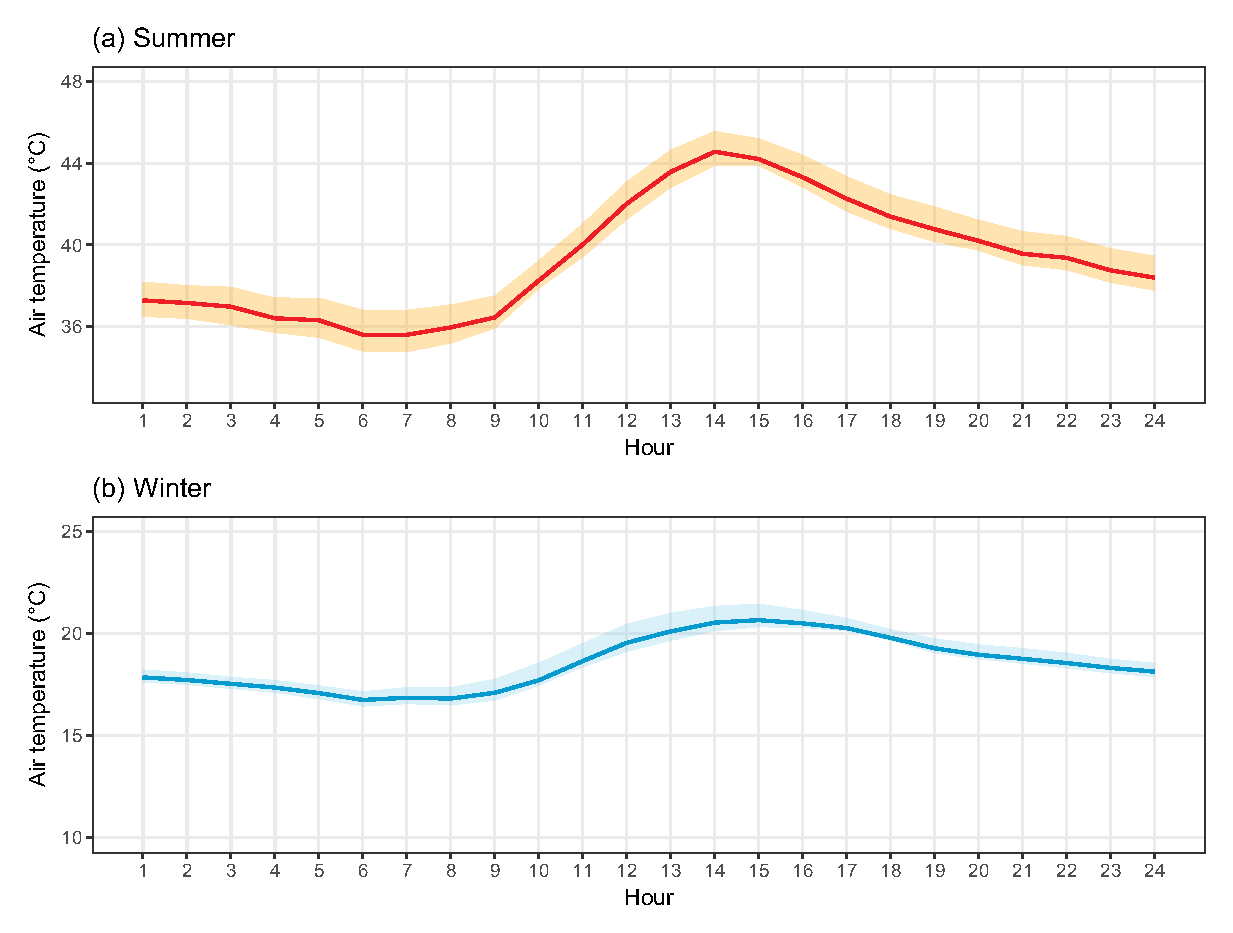
\includegraphics[width=.85\linewidth]{Figure5-1.eps}
\caption{Uncertainty range of the weekly-average diurnal profiles of the predicted urban outdoor air temperature based on Monte Carlo sampling: (a) Results between August 1 and 7, 2017 (summer); (b) Results between February 1 and 7, 2017 (winter). The shaded area represents the predicted values ranging from the 5th to 95th percentile. The solid line represents the predicted values of the 50th percentile.}
\end{figure}

It is interesting to observe that both the predicted summer uncertainty band and diurnal variation are generally larger than the winter ones. A possible reason lies in the seasonal variation of cooling load and solar radiation. During the summer in Abu Dhabi, the cooling demand and solar radiation become very high, resulting in a situation where the HVAC- and radiation-related parameters may have relatively larger impacts on the variation of the microclimate. During the winter, however, the role of these parameters in the urban thermal process becomes quite trivial.

\section{Sensitivity analysis}

Based on the evaluations with a large sample size, it seems reasonable to state that 0.025 (2.5\%) is a sufficient threshold for obtaining good SRC values \cite{saltelli2004sensitivity,menberg2016sensitivity}. Thus we decide that, for the present study, the parameter with an average of the absolute SRCs larger than 2.5\% over 24 hours in one day should have a significant impact on the model output. The resulting hourly coefficients of determination (R$^2$) are summarized in \textbf{Table 5.1}. The generally high R$^2$ values for most hours suggest that the higher-order effects due to non-linear behavior or parameter interaction play a fairly trivial role in the current model setting. This increases our confidence of using the SRC for the sensitivity analysis, which then identified 10 significant parameters for summer and eight for winter in 2017. \textbf{Figures 5-2 and 5-3} plot their hourly SRCs for each group respectively. The results are very consistent with those in our former study \cite{mao2017global} when we performed identical analysis on the same UWG model for summer and winter in 2016.

\begin{table}[]
\footnotesize
\centering
\caption{Coefficient of determination (R$^2$) of the regression model for the weekly-average diurnal profiles of the predicted urban outdoor air temperature during 2017.}
\begin{tabular}{lllllll}
\toprule
Hour & Summer & Winter &  & Hour & Summer & Winter \\ \hline
1    & 0.734  & 0.815  &  & 13   & 0.825  & 0.787  \\
2    & 0.712  & 0.810  &  & 14   & 0.797  & 0.778  \\
3    & 0.735  & 0.830  &  & 15   & 0.701  & 0.760  \\
4    & 0.778  & 0.797  &  & 16   & 0.745  & 0.741  \\
5    & 0.756  & 0.841  &  & 17   & 0.790  & 0.721  \\
6    & 0.815  & 0.855  &  & 18   & 0.796  & 0.738  \\
7    & 0.772  & 0.825  &  & 19   & 0.789  & 0.779  \\
8    & 0.782  & 0.818  &  & 20   & 0.751  & 0.761  \\
9    & 0.790  & 0.810  &  & 21   & 0.772  & 0.771  \\
10   & 0.731  & 0.768  &  & 22   & 0.718  & 0.783  \\
11   & 0.798  & 0.755  &  & 23   & 0.779  & 0.795  \\
12   & 0.837  & 0.783  &  & 24   & 0.770  & 0.807  \\
\bottomrule
\end{tabular}
\end{table}

\begin{figure}[h]
\centering
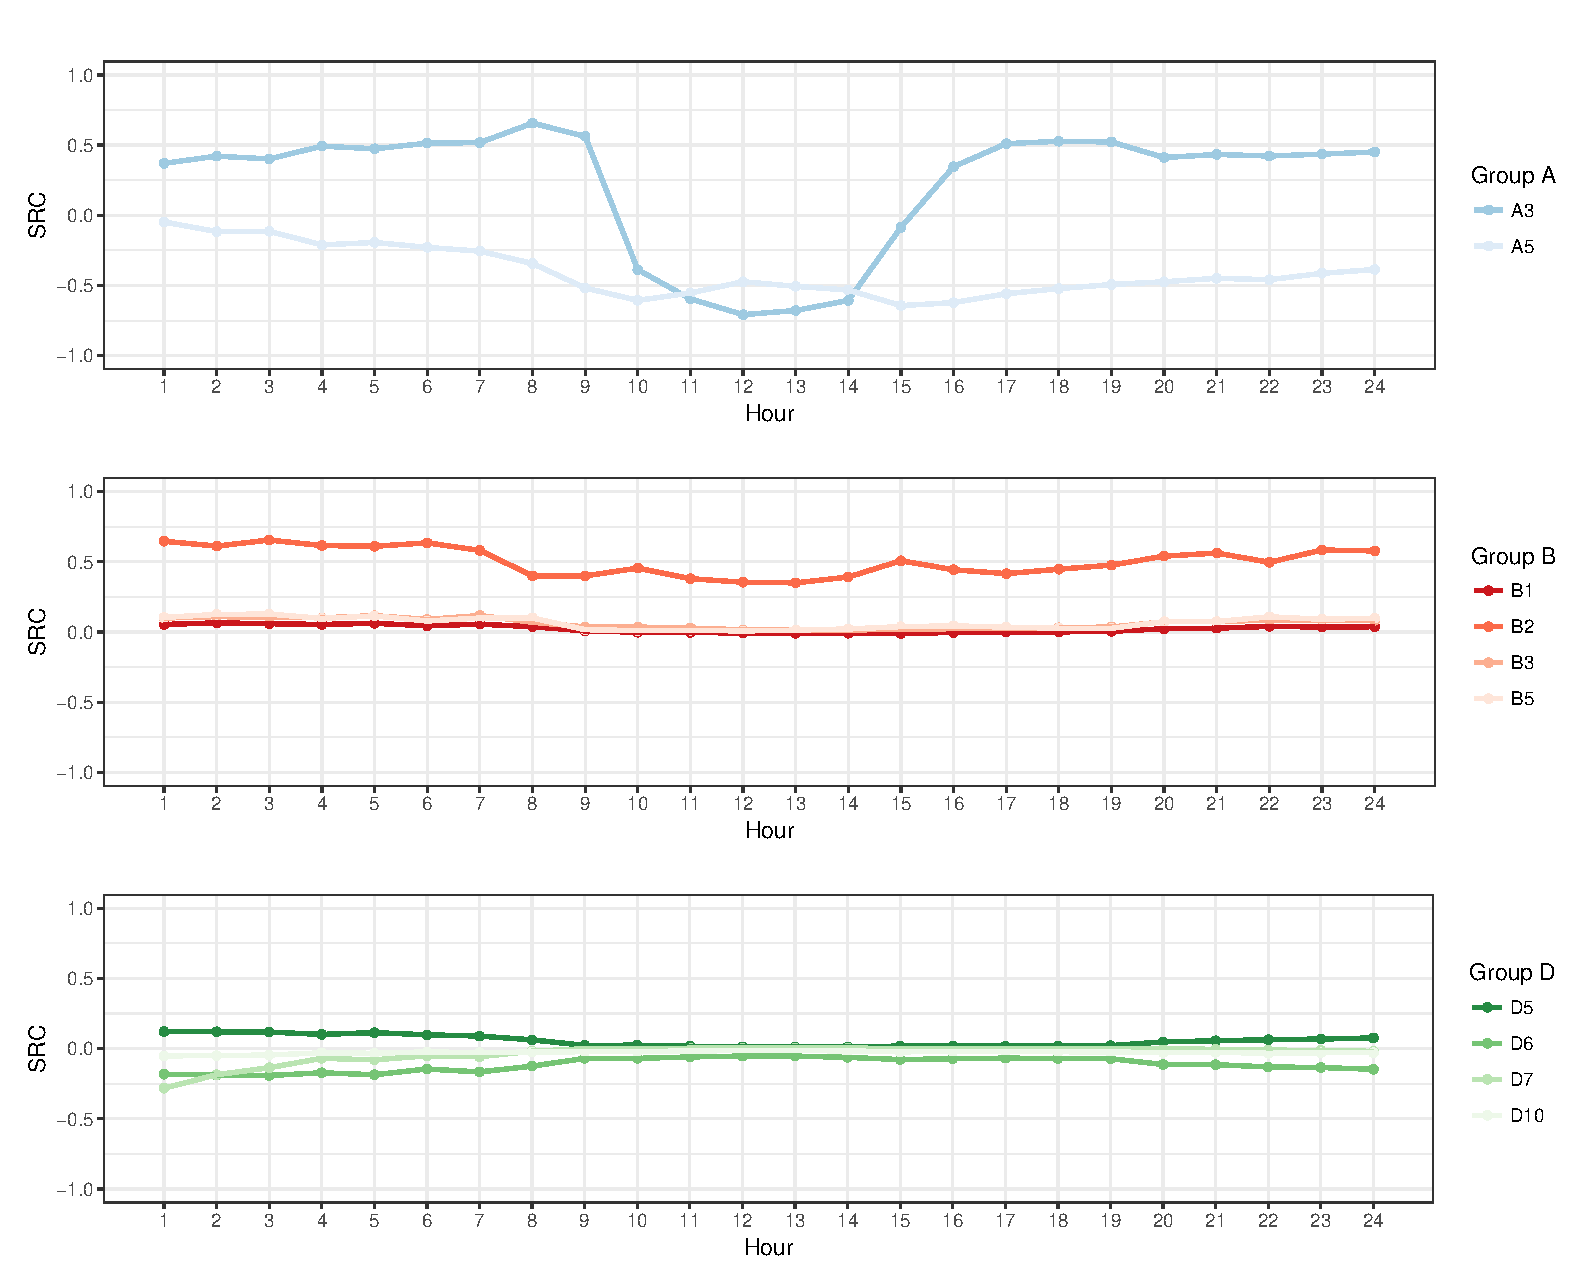
\includegraphics[width=.875\linewidth]{Figure5-2.eps}
\caption{The significant parameters obtained from the global sensitivity analysis of the weekly-average diurnal profiles of the predicted urban outdoor air temperature between August 1 and 7, 2017 (summer). The parameter denotations are the same as those defined in \textbf{Table 4.1}.}
\end{figure}

\begin{figure}[h]
\centering
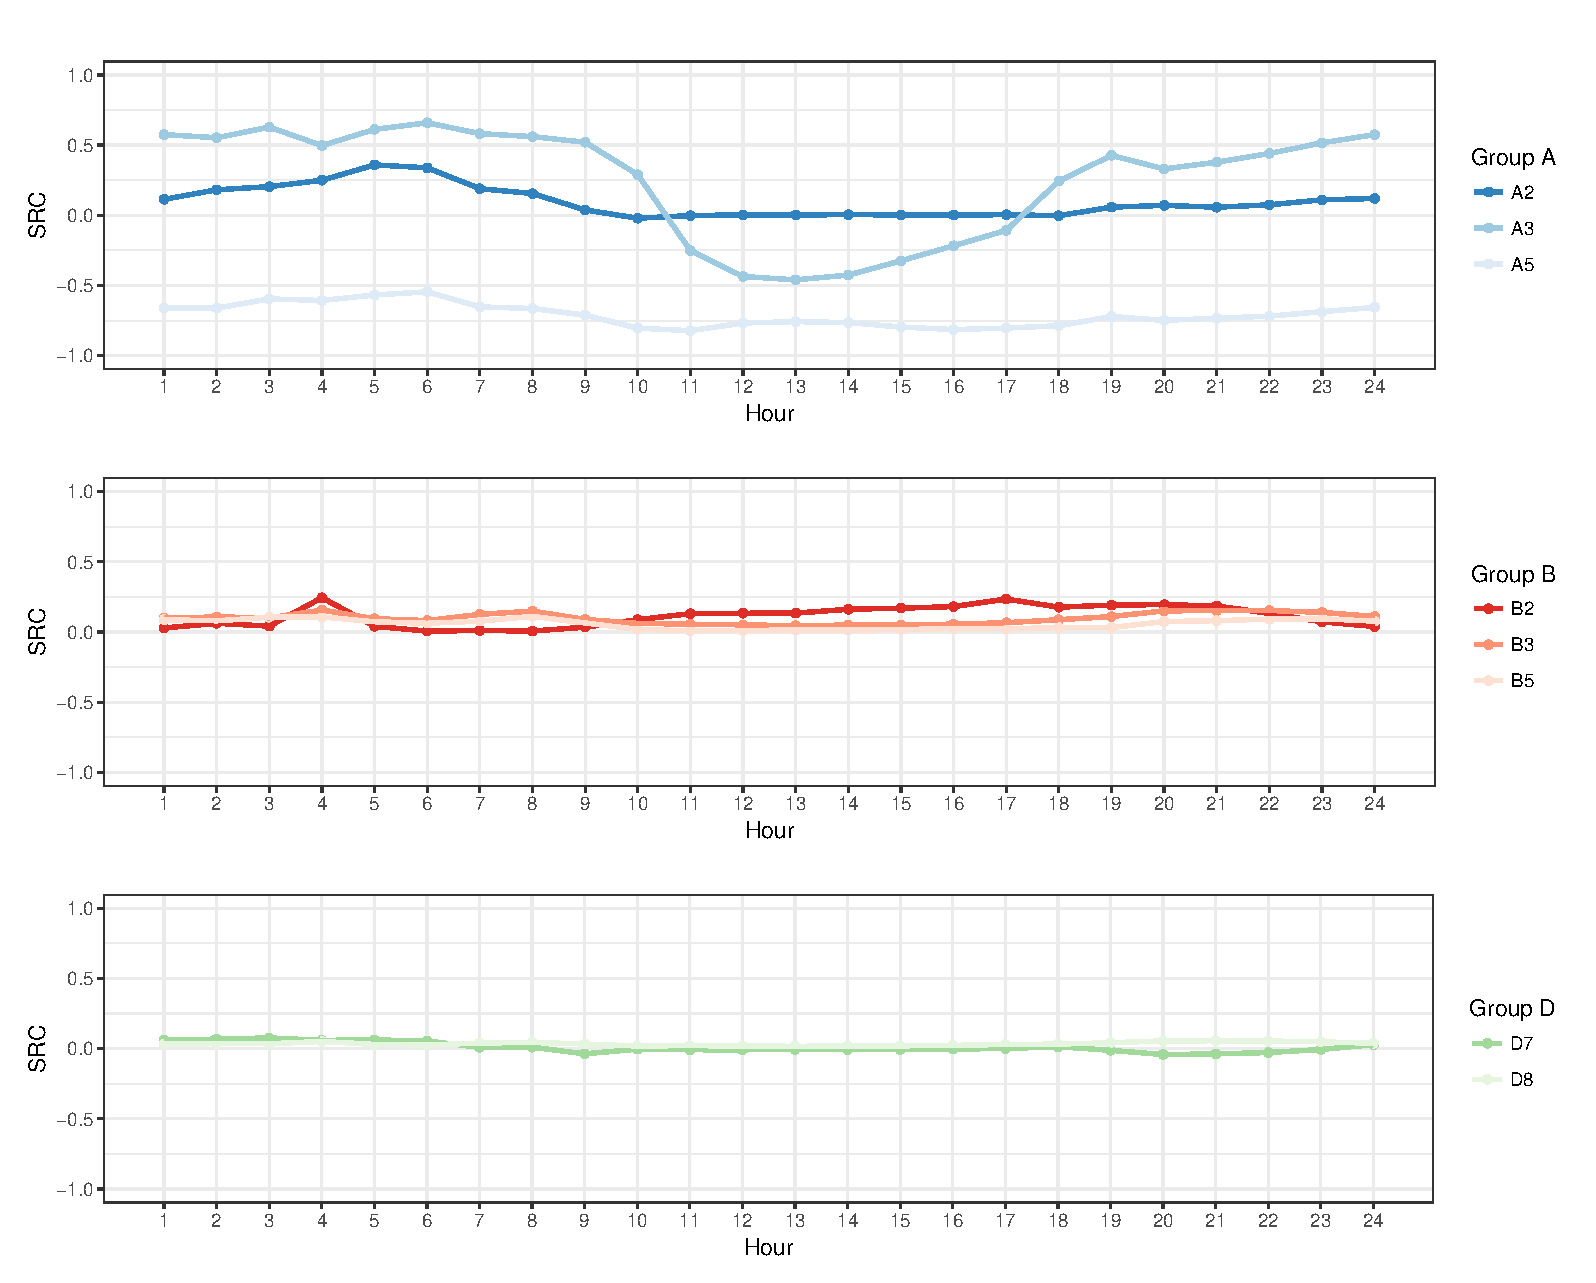
\includegraphics[width=.875\linewidth]{Figure5-3.eps}
\caption{The significant parameters obtained from the global sensitivity analysis of the weekly-average diurnal profiles of the predicted urban outdoor air temperature between February 1 and 7, 2017 (winter). The parameter denotations are the same as those defined in \textbf{Table 4.1}.}
\end{figure}

It is important to mention that no parameter in Group C (vegetation variables) is identified as a strong parameter. This can be explained by the fact that there is nearly no vegetation in Abu Dhabi, thus resulting in relatively smaller uncertainty ranges for the vegetation coverages (see \textbf{Table 4.1}). Previously, Bueno et al. \cite{bueno2013urban} reported that the case study of Basel (Switzerland) is sensitive to some vegetation parameters. We should emphasize that the UHI effect seems to vary locally from one place to another and thus the parameter sensitivity needs to be considered case by case.

It can also be seen from \textbf{Figures 5-2 and 5-3} that although all the parameters have an impact, the most critical ones are the reference height of the VDM (A3), the UCM-UBL exchange coefficient (A5), the fraction of waste heat into canyon (B2), and the nighttime urban boundary layer height (A2, for winter only). Ironically, these parameters remain the most uncertain among all the input variables. The reference height of the VDM and the nighttime urban boundary layer height are obtained from previous mesoscale atmospheric simulations \cite{li2013multi,hidalgo2008urban} because no observations are available. The UCM-UBL exchange coefficient and the fraction of waste heat into canyon are derived from the previous literature \cite{hanna2010wind} and well-educated guesses with limited domain knowledge. Since an urban system is typically characterized by a multiplicity of dynamic (building), stochastic (occupant), and probabilistic (weather) elements, it is difficult to find the exact values for these parameters for a given urban site. In order to capture the site-specific microclimate effects and reduce the uncertainty in the UWG model, additional numerical simulations of the established energy balances might be required. In addition, future improvement of the assessment would be to conduct more detailed estimate of higher-order effects, thus revealing deeper insights into the complex parameter behavior.

Finally, the difference between the summer and winter case suggests that we should focus on different parameters when studying different periods of time. Nevertheless, the identified key factors will be the subject of our subsequent research on the urban microclimate system in Abu Dhabi.

\section{Performance of the Monte Carlo filtering}

\begin{table}[!h]
\footnotesize
\begin{center}
\caption{List of the strong and weak parameters from the Monte Carlo filtering.}
\begin{tabular}{lll}
\toprule
Strong parameter                                  & Unit        & Range            \\ \hline
Nighttime urban boundary layer height (A2)        & m           & {[}50, 100{]}    \\
Reference height of the VDM (A3)                  & m           & {[}100, 200{]}   \\
UCM-UBL exchange coefficient (A5)                 & -           & {[}0.1, 0.9{]}   \\
Average building height (B1)                      & m           & {[}30, 40{]}     \\
Fraction of waste heat into canyon (B2)           & -           & {[}0.1, 0.9{]}   \\
Building density (B3)                             & -           & {[}0.15, 0.35{]} \\
Urban area characteristic length (B5)             & m           & {[}800, 1200{]}  \\
Infiltration rate (D5)                            & ACH         & {[}0.1, 0.7{]}   \\
Chiller COP (D6)                                  & -           & {[}2, 4{]}       \\
Indoor air temperature set point (D7)             & $^{\circ}$C          & {[}20, 24{]}     \\
Equipment load density (D8)                       & W m$^{-2}$       & {[}10, 16{]}     \\
Occupancy density (D10)                           & m$^2$ person$^{-1}$ & {[}15, 25{]}     \\ \hline
\rule{0pt}{2.75ex}Weak parameter                                    & Unit        & Value            \\ \hline
Daytime urban boundary layer height (A1)          & m           & 753.31           \\
Circulation coefficient (A4)                      & -           & 0.98             \\
Heat flux threshold for daytime conditions (A6)   & W m$^{-2}$       & 199.04           \\
Heat flux threshold for nighttime conditions (A7) & W m$^{-2}$       & 50.59            \\
Vertical-to-horizontal ratio (B4)                 & -           & 2.19             \\
Road albedo (B6)                                  & -           & 0.16             \\
Traffic sensible anthropogenic heat (peak) (B7)   & W m$^{-2}$       & 20.35            \\
Urban grass coverage (C1)                         & -           & 0.04             \\
Urban tree coverage (C2)                          & -           & 0.04             \\
Vegetation albedo (C3)                            & -           & 0.25             \\
Latent fraction of grass (C4)                     & -           & 0.61             \\
Latent fraction of tree (C5)                      & -           & 0.70             \\
Rural vegetation coverage (C6)                    & -           & 0.04             \\
Glazing ratio (D1)                                & -           & 0.50             \\
Wall U-value (D2)                                 & W m$^{-2}$ K$^{-1}$   & 2.52             \\
Window U-value (D3)                               & W m$^{-2}$ K$^{-1}$   & 3.18             \\
Window SHGC (D4)                                  & -           & 0.60             \\
Lighting load density (D9)                        & W m$^{-2}$       & 9.90             \\
\bottomrule
\end{tabular}
\end{center}
Note: \\
(a) The values of the weak parameters are set using the average of the top 20 promising input vectors in terms of the GOF. \\
(b) The identified strong parameters along with the associated ranges will be adjusted through an EA-based calibration process.
\end{table}

Given the results of SA, the weak parameters were then removed from the subsequent calibration process. Their static values were determined, somewhat arbitrarily, using the average of the 20 input vectors with the lowest GOFs. In addition, many strong parameters may have associated higher uncertainties and perhaps be more likely in need of tweaking, which can be done through EA-based optimization. The ranges of these to-be-tuned parameters were assigned by considering the uncertainties based on local building design/energy codes, prevailing engineering practices, and our previous investigations \cite{bueno2013urban,bueno2014computationally,nakano2015urban,yang2016curious}. \textbf{Table 5.2} summarizes the current settings to initiate both the traditional and online hyper-heuristic EAs for the following calibration tests. Each strong parameter is bounded via a uniform distribution in order to evaluate the mathematical optimality in terms of calibration performance.

\section{Performance of the online hyper-heuristics}

The overall goal of our calibration method is to minimize the GOF, stated by Equation (4.1), via parameter tuning. The EA is executed to search the design space of the 12 significant parameters identified by the SA. In order to compare the performances of the traditional and online hyper-heuristic EAs, we applied both EAs to the same calibration problem for 10 independent trials. The two EAs have the same settings for crossover operators, mutation operators, elitist strategies, etc.

\begin{figure}[]
\centering
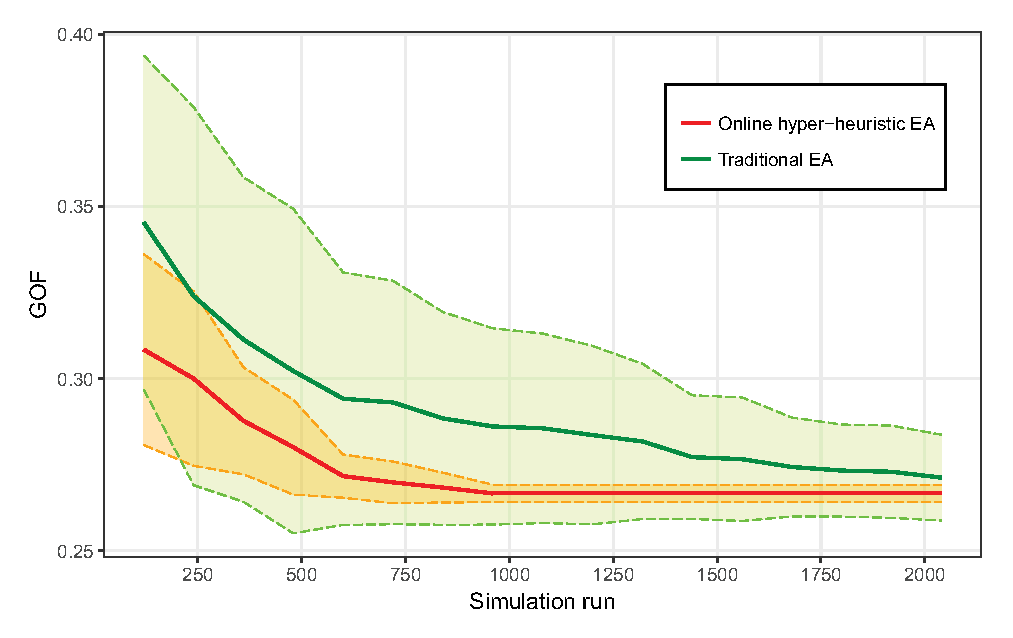
\includegraphics[width=.7\linewidth]{Figure5-4.eps}
\caption{Convergence behavior of the traditional and online hyper-heuristic EAs in terms of the UWG simulation runs (i.e., expensive evaluations). The solid line represents the average of the best fitness values over the 10 trials for the two algorithms, respectively. The shaded area inside the dashed lines represents one standard deviation of the best fitness values over the 10 trials for the two algorithms, respectively.}
\end{figure}

\textbf{Figure 5-4} shows the convergence behavior of the traditional and online hyper-heuristic EAs. For 2040 simulation runs, the online hyper-heuristic EA has, on average, converged to a slightly better near-optimal value than the traditional EA. That is, given the same computation budget, the online hyper-heuristic EA is able to find a slightly better objective value, on average, than the traditional EA for the present case study. In addition, the average number of expensive evaluations (i.e., the UWG simulations) required for the online hyper-heuristic EA to reach a near-optimal value is only around 1000, while that for the traditional EA roughly exceeds 2000. However, it is important to note that \textbf{Figure 5-4} only depicts the number of computationally expensive evaluations (i.e., simulation runs). The online hyper-heuristic EA should require a larger number of objective function evaluations than the traditional EA, because it needs to evaluate an additional surrogate population in each generation. The computation time for the function evaluations in the surrogate is negligible compared with that for the expensive evaluations via the UWG, even though the number of additional function evaluations in the surrogate is large. One could also compute the total number of function evaluations, including both expensive and surrogate evaluations, to see the difference (an option for future work), but what really matters in practice is the number of expensive evaluations during a simulation-based optimization. Therefore, the online hyper-heuristic EA seems to be about \textit{twice} as fast, on average, as the traditional EA for the same level of accuracy. In this case study, where a single simulation costs about two minutes on a single thread, using the online hyper-heuristic EA can approximately save at least one day, on average, for one calibration trial if no parallel computation is applied.

In addition, the optimum uncertainties of the two EAs (i.e., the shaded area inside the dashed lines in \textbf{Figure 5-4}) are quite different. Over these 10 trials, the online hyper-heuristic EA has a smaller uncertainty band, especially after $\sim$1000 expensive evaluations, which means that the results of one single trial of the online hyper-heuristic EA are more reliable and robust. In contrast, the traditional EA yields a much wider uncertainty band, which somewhat compromises the best fitness value identified in only one calibration trial. In single-objective optimization, a well-performed EA can produce most solutions that are expected to be clustered around the global optimum. Some others could be clustered around local optima and some outlying individuals may exist as well. Outliers are generated due to mutation, which intends to prevent the solution from being trapped in local optima. Searching solutions mostly in a specific parameter space would act in favor of the online surrogate model, whose predictive capability is progressively increased as more objective functions are evaluated. Therefore, the online hyper-heuristics can fairly produce more confident solutions when computation time is limited.

The solutions obtained from both the traditional and online hyper-heuristic EAs are summarized in \textbf{Table 5.3}. We found great consistency between the two algorithms over 10 trials, leading us to conclude that the EA is able to identify the sub-ranges of most strong parameters in our current settings. Besides, the solution uncertainties from the online hyper-heuristic EA are, in general, smaller than those from the traditional EA. This reinforces our argument that, in single-objective optimization, the online surrogate model can help EA produce the solutions that are robustly closer to the global optimum with much less computation time.

\begin{table}[]
\footnotesize
\begin{center}
\caption{Calibration results over the 10 trials of EA-based optimization.}
\makebox[\linewidth]{
\begin{tabular}{llll}
\toprule
Parameter                                  & Unit        & \vtop{\hbox{\strut Result from}\hbox{\strut traditional EA}}  & \vtop{\hbox{\strut Result from online}\hbox{\strut hyper-heuristic EA}}  \\ \hline
Nighttime urban boundary layer height (A2) & m           & 79.51 $\pm$ 13.92              & 89.57 $\pm$ 9.98                          \\
Reference height of the VDM (A3)           & m           & 171.96 $\pm$ 29.09             & 195.09 $\pm$ 11.86                        \\
UCM-UBL exchange coefficient (A5)          & -           & 0.10 $\pm$ 0.00                & 0.10 $\pm$ 0.00                           \\
Average building height (B1)               & m           & 34.48 $\pm$ 2.42               & 35.68 $\pm$ 1.16                          \\
Fraction of waste heat into canyon (B2)    & -           & 0.14 $\pm$ 0.03                & 0.16 $\pm$ 0.01                           \\
Building density (B3)                      & -           & 0.33 $\pm$ 0.02                & 0.33 $\pm$ 0.01                           \\
Urban area characteristic length (B5)      & m           & 1116.43 $\pm$ 108.50           & 1176.47 $\pm$ 29.97                       \\
Infiltration rate (D5)                     & ACH         & 0.24 $\pm$ 0.13                & 0.15 $\pm$ 0.09                           \\
Chiller COP (D6)                           & -           & 3.25 $\pm$ 0.87                & 3.86 $\pm$ 0.05                           \\
Indoor air temperature set point (D7)      & $^{\circ}$C          & 21.22 $\pm$ 1.50               & 20.65 $\pm$ 1.05                          \\
Equipment load density (D8)                & W m$^{-2}$       & 14.19 $\pm$ 1.09               & 14.45 $\pm$ 0.43                          \\
Occupancy density (D10)                    & m$^2$ person$^{-1}$ & 20.13 $\pm$ 3.09               & 22.43 $\pm$ 0.93                          \\
\bottomrule
\end{tabular}
}
\end{center}
Note: The results are presented as ``average $\pm$ one standard deviation'' from the solutions over the 10 trials for the two algorithms, respectively.
\end{table}

One interesting observation in \textbf{Table 5.3} is that neither algorithm is able to identify an appropriate sub-range for some parameters (e.g., D5), since the corresponding standard deviation is quite comparable to the average value. On the other hand, the optimal solution of other parameters (e.g., A5) can be determined almost surely. Under a modern optimization lens, there are two possible reasons. First, if the objective function is not quite as sensitive to the parameter (compared to other parameters), its solution could be easily varied during a purely mathematical search and the resulting uncertainty would become large. Second, even if the parameter is quite influential, an algorithm may still fail to reach a single optimal or near-optimal region, since the objective function with respect to this parameter could be highly non-convex, multi-modal, and/or locally-flat. Thus, the observed uncertainties from purely mathematical search in this study would naturally come up with an appealing motivation to investigate the convexity of the target parameter space in urban-scale simulation settings. Future studies could be considered along this direction.

Whether the proposed algorithm's performance can be considered ``good'' from the perspective of why the calibration was considered in the first place is addressed in the next subsection.

\section{Performance of the calibrated model}

Now we analyze in more detail the behavior of the solutions obtained from the online hyper-heuristic EA. Given the measured data at hand, four periods in 2017 are considered for validation of the calibrated UWG models, i.e., January 15-21, February 8-14, July 15-21, and August 8-14. Based on the assumption that the measurement uncertainties impose a limit to the model accuracy that one could hope to achieve, we compared the values measured by the sensors, the values predicted by the optimization-calibrated models, and the values predicted by the manually-calibrated baseline model (detailed in \textbf{Tables 3.1 and 3.3}). The final results are shown in \textbf{Figure 5-5} and \textbf{Table 5.4}, where the accuracy is assessed in terms of how close the predicted values are to the measured values and whether the uncertainty bands are narrow enough to be of practical use while bounding the measurements.

\begin{figure}[]
\centering
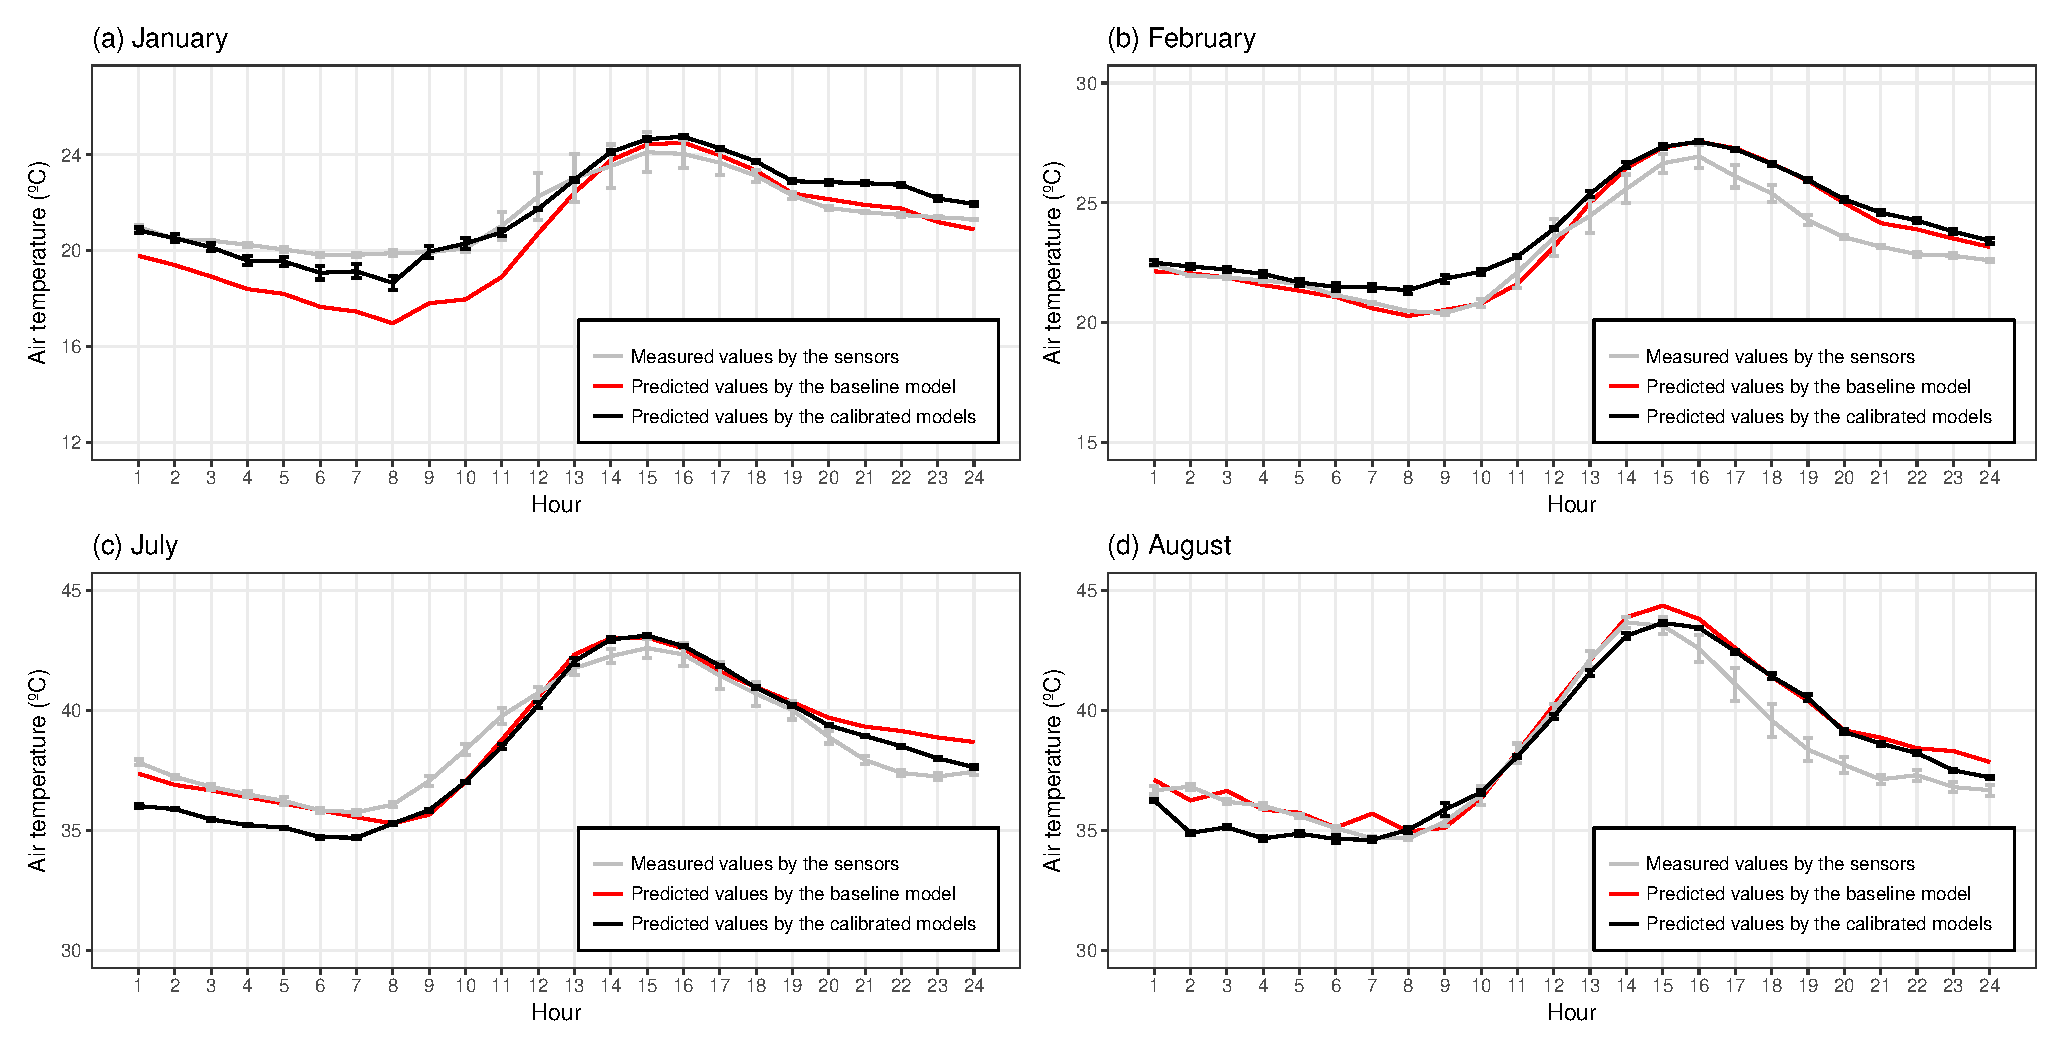
\includegraphics[width=\linewidth]{Figure5-5.eps}
\caption{Weekly-average diurnal profiles of the urban outdoor air temperature: (a) Data between January 15 and 21, 2017; (b) Data between February 8 and 14, 2017; (c) Data between July 15 and 21, 2017; (d) Data between August 8 and 14, 2017. The error bar represents one standard deviation of the measured values by the sensors and the predicted values by the 10 calibrated models, respectively. The baseline model has been manually calibrated via detailed investigations.}
\end{figure}

\begin{table}[]
\footnotesize
\begin{center}
\caption{Performance of the baseline and calibrated UWG models based on two weekly-average diurnal profiles of the urban-rural outdoor air temperature difference.}
\makebox[\linewidth]{
\begin{tabular}{llll}
\toprule
\textbf{Scenario}                                                 & \textbf{January 15-21}                          \\ \hline
Evaluation metric                                        & NMBE          & CV(RMSE) & GOF           \\ \hline
Measured values \textit{v.s.} predicted values (baseline model)   & -0.27         & 0.43     & 0.29          \\
Measured values \textit{v.s.} predicted values (calibrated model) & 0.05          & 0.21     & \textbf{0.08} \\ \hline
\rule{0pt}{2.75ex}\textbf{Scenario}                                                 & \textbf{February 8-14}                          \\ \hline
Evaluation metric                                        & NMBE          & CV(RMSE) & GOF           \\ \hline
Measured values \textit{v.s.} predicted values (baseline model)   & 0.36          & 0.69     & \textbf{0.40}  \\
Measured values \textit{v.s.} predicted values (calibrated model) & 0.77          & 0.90      & 0.78          \\ \hline
\rule{0pt}{2.75ex}\textbf{Scenario}                                                 & \textbf{July 15-21}                             \\ \hline
Evaluation metric                                        & NMBE          & CV(RMSE) & GOF           \\ \hline
Measured values \textit{v.s.} predicted values (baseline model)   & 0.18          & 1.06     & \textbf{0.38} \\
Measured values \textit{v.s.} predicted values (calibrated model) & -0.41         & 1.22     & 0.55          \\ \hline
\rule{0pt}{2.75ex}\textbf{Scenario}                                                 & \textbf{August 8-14}                            \\ \hline
Evaluation metric                                        & NMBE          & CV(RMSE) & GOF           \\ \hline
Measured values \textit{v.s.} predicted values (baseline model)   & 0.57          & 0.87     & 0.61          \\
Measured values \textit{v.s.} predicted values (calibrated model) & 0.17          & 0.89     & \textbf{0.33} \\
\bottomrule
\end{tabular}
}
\end{center}
Note: For the measured values by the sensors and predicted values by the calibrated models, we use the average to evaluate the performance. The bold type highlights which model performs better in terms of the GOF for each scenario. The baseline model has been manually calibrated via detailed investigations.
\end{table}

Overall, the calibrated solutions (black curve) produce weekly-average diurnal profiles of the urban outdoor air temperature similar to the baseline solution (red curve), as shown in \textbf{Figure 5-5}. Sometimes the calibrated models represent the observed behavior better than the baseline model (e.g., January). This is very encouraging since the baseline model has been manually refined and calibrated for over one year via exhaustive investigations of the local construction documents, regular on-site visits, and detailed discussions with experienced engineers and building management personnel. In addition to the performance guarantee from the calibrated models, one great advantage of the methodology proposed in this study lies in the time consumed to obtain them. For this case study, a total of only $\sim$1000 simulations (which take at most two days without parallel computing) on average have resulted in an improved urban microclimate model. So, it seems highly cost-effective and convenient to use the developed algorithm in the process of model calibration.

A further consideration of the hourly data is shown in \textbf{Figure 5-6}, where four days in each validation period are depicted. In general, the calibrated solutions are able to capture most trends as well as peaks and valleys of the measurements. This is impressive because in this study we calibrated the model parameters for a whole year based on just two weekly-average diurnal profiles of the urban-rural outdoor air temperature difference. More data with higher spatial and temporal resolution are being collected and it is reasonable to expect that, if these data were used to calibrate the model, the resulting solutions could achieve higher accuracies with lower uncertainties. Whether the improved performance is commensurate with the extra resources and efforts required to perform accurate measurement and conduct optimization-aided calibration on urban-scale models is not clear and should be investigated in the future.

\begin{figure}[!h]
\centering
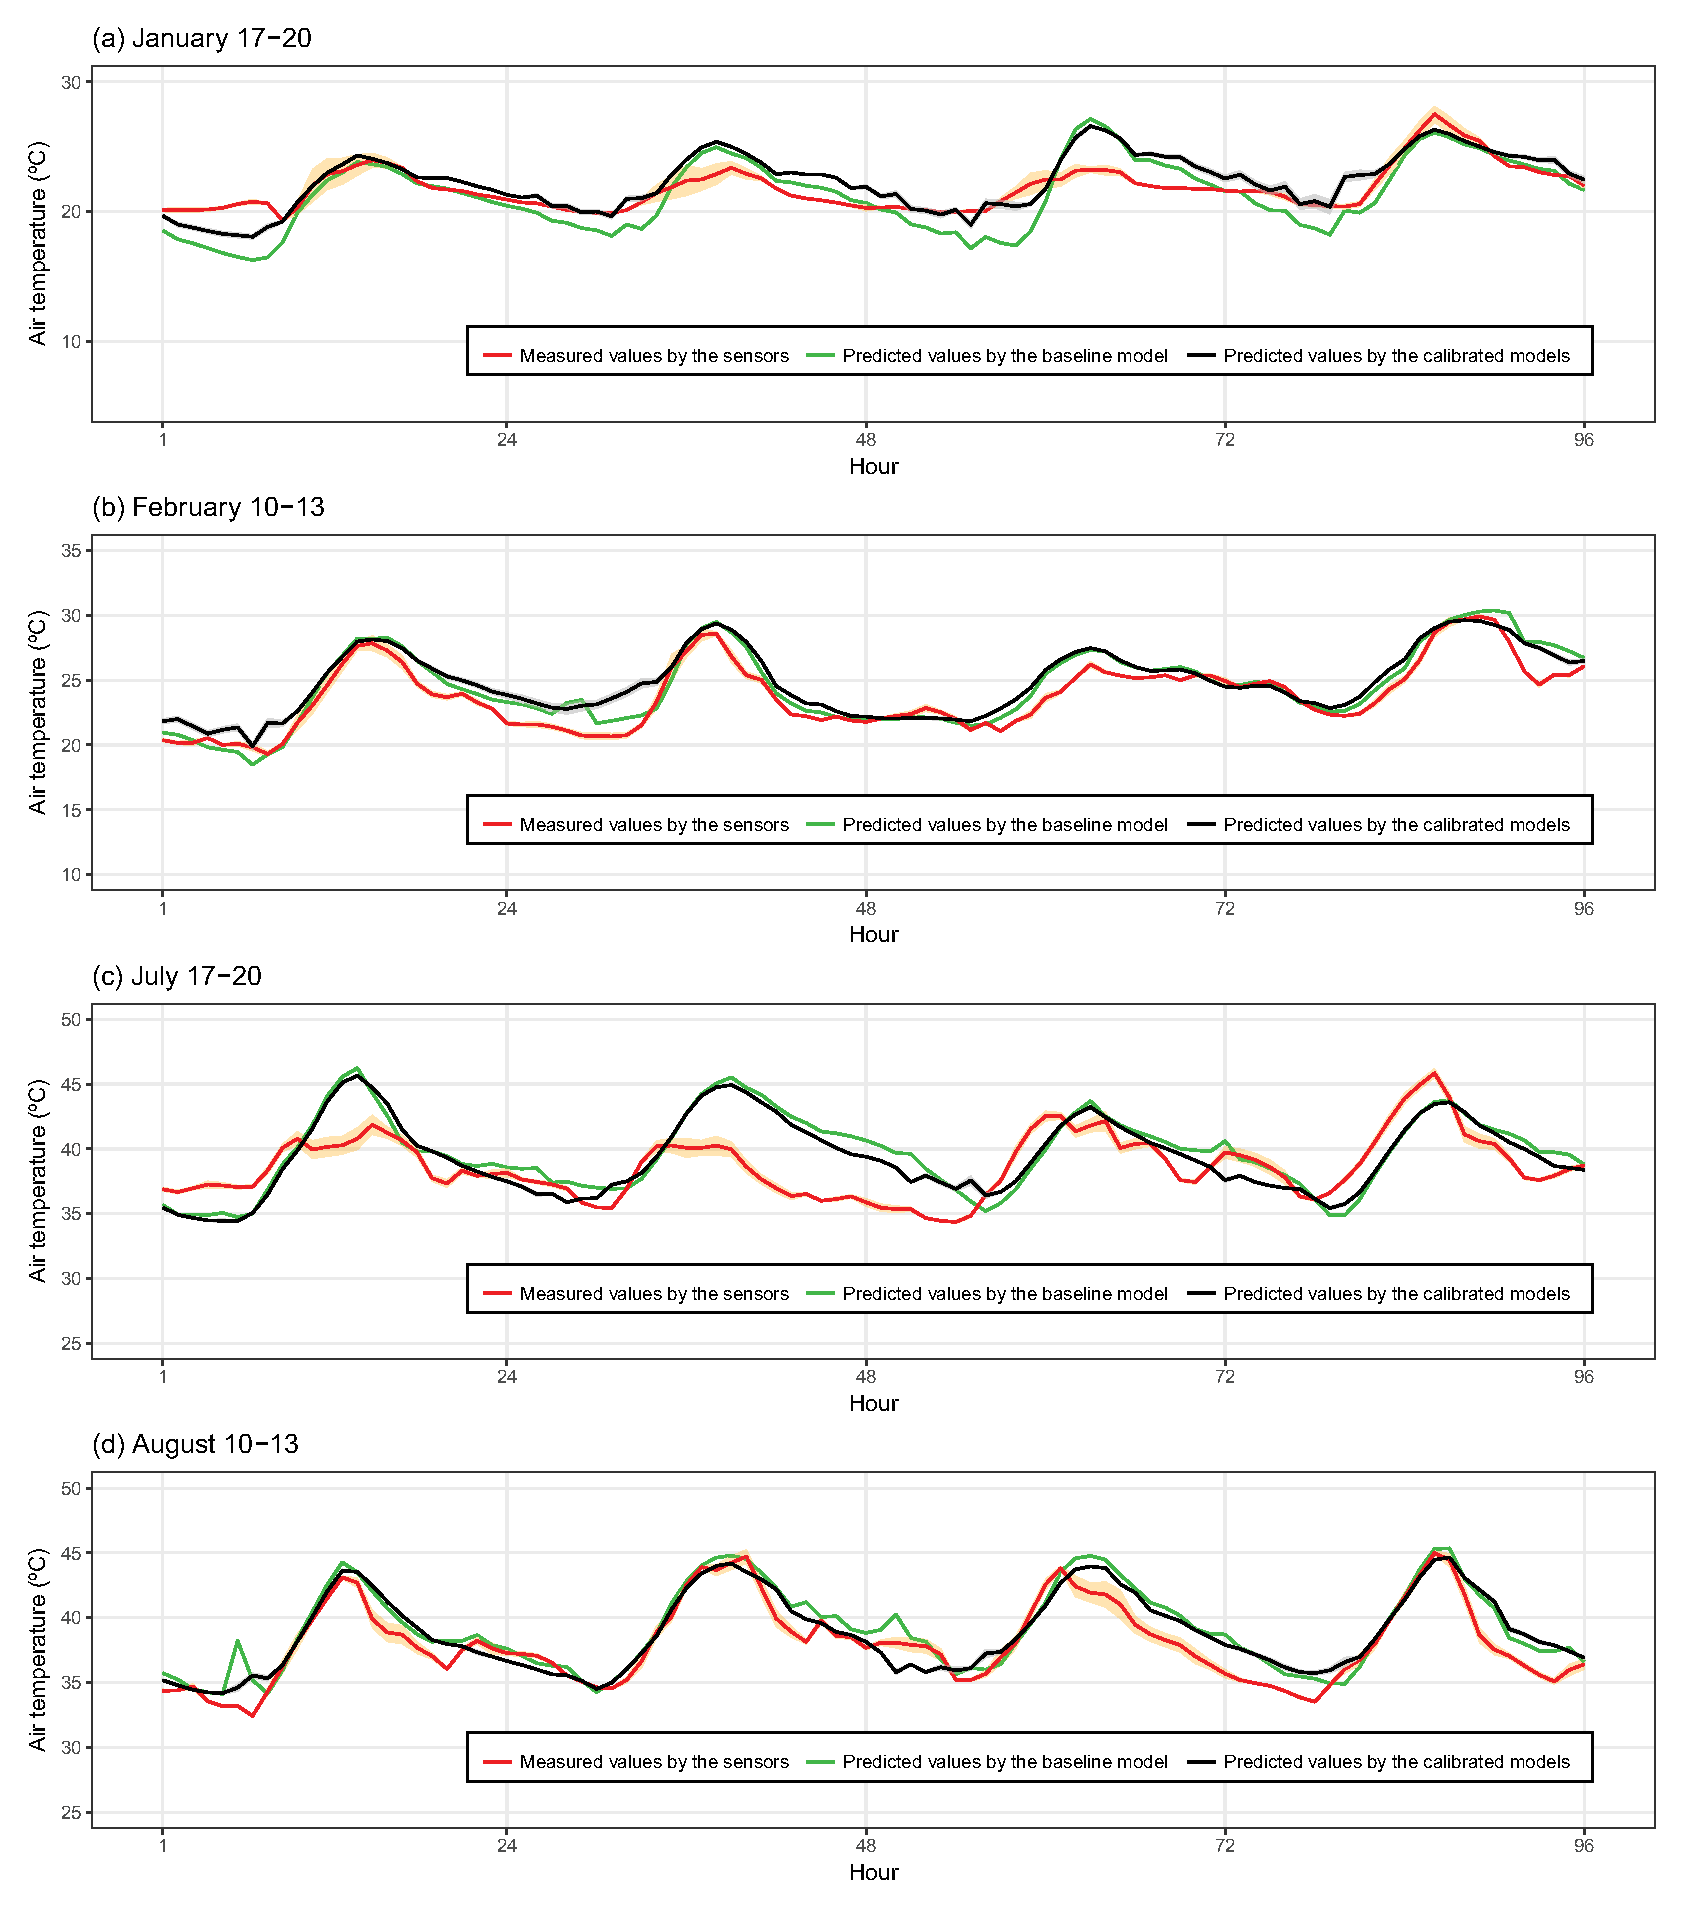
\includegraphics[width=.95\linewidth]{Figure5-6.eps}
\caption{Hourly diurnal profiles of the urban outdoor air temperature in 2017. The solid line represents the average of the measured values by the sensors and the predicted values by the 10 calibrated models, respectively. The shaded area represents one standard deviation of the measured values by the sensors and the predicted values by the 10 calibrated models, respectively. The baseline model has been manually calibrated via detailed investigations.}
\end{figure}

Finally, one particular aspect to notice in \textbf{Figure 5-6} is the unexpected behavior during July 17-18, where large discrepancies between predicted and measured data are evident. A good fit to the weekly-average diurnal profile (i.e., the one with low GOF shown in \textbf{Figure 5-5}) may not necessarily predict the hourly diurnal profile more accurately. One possible reason is that, there may be some short-term physical activities (e.g., anomalous wind patterns) during that time which can largely affect the corresponding urban microclimate condition, while such physical activities have not been adequately modeled in the current UWG or have not been reflected in the given rural weather data. This strong bias needs to be revisited in our future studies and may call into question a conclusion from a previous UWG assessment that the location of the reference station has minimal impact on the estimate of temperatures at district level because the urban-canopy energy balance is weakly influenced by advection in the urban boundary layer \cite{bueno2014computationally}. Nevertheless, in most cases, the differences are quite acceptable given the state of the art of urban microclimate modeling.




\chapter{Conclusion}

\AddToShipoutPictureBG*{%
  \AtPageUpperLeft{%
    \hspace*{18.275cm}%
    \raisebox{-3.55cm}{%
      \makebox[0pt][r]{\parbox{\textwidth}{\begin{flushright}\textit{``Now this is not the end. \\It is not even the beginning of the end. \\But it is, perhaps, the end of the beginning.''}\\
      Winston Churchill\end{flushright}}}
}}}%

The extreme complexity of a building or urban system leads to difficulties in estimating the benefits and drawbacks of present and future adaptation strategies to climate change and energy concern. The design, analysis, and optimization of modern building and urban systems may benefit significantly from the implementation of energy and environmental simulation tools at different scales. However, in many cases, studies have revealed large discrepancies between modeled and measured values, which somewhat undermines our confidence in the practical value of these simulation tools. A well-calibrated model is hence one of the key bases for practitioners to perform simulation-based analysis.

This thesis illustrates a general methodology for automatic model calibration and, for the first time, applies it to an existing urban microclimate system. This chapter summarizes the key conclusions.

\section{Summary of contributions}

We started by recognizing that calibration remains an indeterminate and/or over-parametrized problem which could yield non-unique solutions. Hence, it is more reasonable to identify a set of most plausible solutions and to incorporate uncertainty when evaluating and using a calibrated model. In general, we performed global sensitivity analysis, Monte Carlo filtering, and optimization-aided calibration on a microclimate model using the measurements in 2017. Due to the time-constrained nature of engineering applications, an online hyper-heuristic evolutionary algorithm (EA) is proposed and developed to accelerate the calibration process.  Validation of the proposed methods was more of an empirical nature.

The Urban Weather Generator (UWG) \cite{bueno2013urban} is selected as the simulation engine in the present study. The UWG can be used as a physics-based model to produce the microclimate condition at the urban street level by using the meteorological information in available rural weather files. It can also be used as a bottom-up model to estimate the urban energy consumption by aggregating the building stocks. Since the previous version in 2014 \cite{bueno2014computationally}, the UWG has been updated, especially for the urban boundary layer model and the urban canopy-building energy model \cite{yang2016curious}. In general, the newest version aims to make it more physically sound and more capable to handle increasingly detailed building definition.

The District E3 in downtown Abu Dhabi provides a test to the new UWG with an interesting case of heterogeneous building forms located in a tropical or subtropical climate zone. The comparison between the measurements and the predictions by a baseline model from October to December 2016 shows that the UWG can roughly capture the UHI pattern and can produce some plausible values regarding the urban microclimate condition. Thus, together with previous studies \cite{bueno2013urban,bueno2014computationally,nakano2015urban,yang2016curious}, the UWG model can be applied to different climate zones and urban configurations to yield an estimation of the UHI effect.

The regression-based analysis with Monte Carlo sampling is then used to quantify the model uncertainty and to identify significant parameters for summer and winter in 2017, based on 30 candidate inputs from the meteorological factors, urban characteristics, vegetation variables, and building systems. The uncertainty analysis indicates that the UWG is a fairly robust simulator to approximate the thermal behavior of the urban microclimate system in Abu Dhabi for different seasons. It is interesting to observe that both the predicted summer uncertainty band and diurnal variation are generally larger than the winter ones.

The parameter ranking based on the standardized regression coefficients (SRCs) from the linear regression suggests that no vegetation parameter has been identified as a strong parameter in Abu Dhabi during 2017. The most critical parameters are the reference height of the VDM, the UCM-UBL exchange coefficient, the fraction of waste heat into canyon, and the nighttime urban boundary layer height (for winter only). Ironically, these parameters remain the most uncertain among all the input parameters, calling for further investigations into their physical mechanism. Overall, the regression-based analysis is able to identify 12 strong parameters for summer and winter. These 12 parameters are then considered in an optimization-aided calibration process based on the measurements in one summer week and one winter week during 2017.

The proposed online hyper-heuristic EA is roughly twice as fast, on average over 10 trials for the present case study, as the traditional EA to achieve the same objective. In addition, both algorithms are able to identify the sub-ranges of most strong parameters in our current settings, while the solutions from the online hyper-heuristic EA have generally smaller uncertainties. In single-objective optimization, searching solutions mostly in a specific parameter space would act in favor of the online hyper-heuristics, which can thus help EA produce the solutions that are robustly closer to the global optimum with much less computation time.

The solutions obtained from the online hyper-heuristic EA can produce weekly-average diurnal profiles of the urban outdoor air temperature similar to the manually-calibrated baseline solution, which has been extensively investigated for over one year. This is encouraging because a total of only $\sim$1000 simulations (which take at most two days without parallel computing for the present study) could result in an improved urban microclimate model. In addition, the calibrated solutions are able to capture most trends as well as peaks and valleys of the measured data on an hourly basis for certain periods of the year. Despite some yet unexplained behaviors, the calibrated models generally perform well. Therefore, the automatic calibration method proposed in this study is expected to improve the model performance to some extent, both effectively and efficiently.



\section{Discussion and future work}

For simulation-based optimization problems, hyper-heuristics have a catalytic effect in obtaining solutions, but have been overshadowed by the success of parallel computing \cite{zhang2009parallel}. Indeed, some researchers have recently tried to improve the run-time of optimization algorithms via surrogate models \cite{eisenhower2012methodology,boithias2012genetic,vcongradac2012recognition}. However, most studies focused on offline hyper-heuristics where a surrogate or meta-model is trained in advance. This would require additional effort to build a database for a specific case study and the algorithm cannot fully guarantee equivalent quality solutions if the true simulation engine is discarded. Online hyper-heuristics, on the other hand, have a self-updating mechanism without any pre-simulated database to produce well-verified solutions \cite{brownlee2015constrained,xu2016improving}. Therefore, we advocate the use of online hyper-heuristics among relevant research communities that are interested in simulation-based optimization.

The present study only considered a model calibration based on the urban outdoor air temperature via single-objective optimization. Energy use or other urban microclimate conditions (e.g., air humidity) at multi-layer level could be further incorporated into the calibration process if the corresponding data were available at sufficiently high frequency. Given hourly or sub-hourly data of the outdoor microclimate and/or building energy use in an urban neighborhood, one could conduct simultaneous model calibration via multi-objective optimization (MOO) \cite{santos2018evaluating}. The performance of the online hyper-heuristic EA could be further evaluated in this MOO setting. Another direction for future studies would be to develop automatic pattern-based calibration methods \cite{sun2016pattern} or Bayesian calibration methods \cite{heo2012calibration} in order to further improve the results from a purely heuristic-based search. A joint mathematics- and physics-based calibration approach that is able to effectively integrate the actual measurements and computer simulations has the potential to improve the way building and urban systems are designed and operated.

At a more fundamental and philosophical level, any comparison between the predicted and measured performance could be viewed in terms of not only how well the simulation agrees with the measurement, but also \textit{whether the simulation program is good enough for its intended purposes} \cite{reddy2007calibrating}. The question of interest is, then, how to determine a ``good enough'' solution? In particular, there should be a broad consensus among the scientific and engineering communities when it comes to the specification of the accuracy bound at different scales for the calibration to be deemed satisfactory. Scientists prefer to describe such bound as \textit{uncertainty}, which is one key idea we want to deliver in this thesis. The input uncertainties indicate the difficulties in capturing the inherent physical properties (e.g., model parameter values) during a specific simulation setting. It is assumed that, if the model is calibrated within the prescribed criteria, it seems closer to the physical reality as the input parameters (i.e., the ``knobs'') are tuned properly.

However, just because all the selected knobs yield a desired output, we cannot guarantee that each knob is tuned correctly \cite{reddy2007calibrating}. Most simulation models have many degrees of freedom and, with judicious fiddling, can be easily manipulated to produce any desired behavior with both plausible model structures and parameter values. More often than not, this calibration process can be seen as GIGO (garbage in, garbage out) \cite{saltelli2008global}. The reason may lie in the fact that, during an optimization process, we usually obtain one specific parameter combination leading to a ``local'' optimum within the search space. Thus, the output (or solution) uncertainties, which demonstrate the consistency of a calibration process, should also be considered with great care after calibration. Earlier, Kaplan et al. \cite{kaplan1990reconciliation} looked at this issue and concluded that one can never hope to identify the parameters correctly, in part because we do not know what is correct. Given this unanswerable (and maybe hopeless) situation, limiting ourselves to one plausible solution would be quite misleading. It is hence much more reasonable to incorporate both the input and output uncertainties when evaluating and using a calibrated model. 

The present study has not considered the parameters of the rural measurement, which might be an interest of research in the future if sufficient data is available. In addition, to incorporate the actual effect on an urban system due to occupancy, we might need to combine the UWG with reliable stochastic occupant behavior models \cite{hong2017ten}. Finally, the energy flow process modeled by the current UWG from the rural station to the urban canopy may not be a complete mechanism to depict the physics of the urban microclimate, even though most UWG outputs seem reasonable and the intended purposes of UWG have been fulfilled to some extent. Numerical CFD simulations might be further needed to illustrate whether the actual interaction between the air masses in the rural and urban area has been accurately formulated for a specific city.

%\let\cleardoublepage\clearpage
\newpage
\mbox{}
%\appendix
\chapter*{Nomenclature}
\addcontentsline{toc}{chapter}{Nomenclature}
\noindent
\begin{tabular}{p{3.5cm}p{11.5cm}}
$A_f$ & lateral heat exchange area (m$^2$) \\
$c_p$ & specific heat of air at constant pressure (J kg$^{-1}$ K$^{-1}$) \\
$c_v$ & specific heat of air at constant volume (J kg$^{-1}$ K$^{-1}$) \\
$D$ & training database \\
$F_{E,P}/F_{E,Q}$ & expensive objective and constraint values in $P/Q$ \\
$F_S$ & approximated objective and constraint values in $S$ \\
$h_{bld}$ & average building height (m) \\
$H_u$ & sensible heat flux at the surface of the control volume (W) \\
$K_{r,dir}/K_{w,dir}$ & fraction of the direct solar radiation received by the road/wall\\
$\bar{m}$ & mean of the absolute measured urban-rural temperature differences \\
$m_i$ & measured data point $i$ of the urban-rural temperature difference \\
$n$ & number of the data points \\
$P$ & parent population \\
$Q$ & offspring population \\
$Q_{LW,down}$ & down-welling infrared radiation specified in the EPW file (W) \\
$Q_{LW,road}/Q_{LW,roof}/Q_{LW,wall}$ & \qquad \qquad \qquad long-wavelength heat exchange between the atmosphere and the road/roof/wall (W) \\
R$^2$ & coefficient of determination\\
$r_{aspect}$ & aspect ratio\\
$r_{shade}$ & fraction of the road shaded by trees\\
$S$ & surrogate population \\
$S_{hor,dir}$ & direct solar radiation on a horizontal surface (W m$^{-2}$)\\
$S_{norm,dir}$ & direct normal solar radiation (W m$^{-2}$)\\
$s_i$ & simulated data point $i$ of the urban-rural temperature difference \\
$t$ & generation counter \\
$T_{road}/T_{roof}/T_{wall}$ & surface temperature of the road/roof/wall (K)\\
\multicolumn{2}{c}{}
\end{tabular}

\noindent
\begin{tabular}{p{3.5cm}p{11.5cm}}
$u_{ref}$ & reference air velocity (m s$^{-1}$)\\
$V_{CV}$ & control volume (m$^3$)\\
$VF_{i-j}$ & view factor from $i$ to $j$\\
$w_{\textrm{CV(RMSE)}}/w_{\textrm{NMBE}}$ & weight assigned to CV(RMSE)/NMBE \\
$w_r$ & average road width (m)\\
\multicolumn{2}{c}{}
\end{tabular}


\section*{Greek symbol}

\begin{tabular}{p{3.5cm}p{11.5cm}}
$\epsilon_{road}/\epsilon_{roof}/\epsilon_{wall}$ & emissivity of the road/roof/wall \\
$\theta_0$ & critical canyon orientation \\
$\theta_{ref}$ & reference potential temperature outside the control volume (K)\\
$\theta_u$ & average potential temperature of the control volume (K)\\
$\lambda$ & solar zenith angle\\
$\rho$ & air density (kg m$^{-3}$)\\
$\sigma$ & Stefan-Boltzmann constant (W m$^{-2}$ K$^{-4}$) \\
\multicolumn{2}{c}{}
\end{tabular}

\section*{Abbreviation}

\begin{tabular}{p{3.5cm}p{11.5cm}}
AEC & architecture, engineering, and construction \\
AM & averaged model\\
ASHRAE & American Society of Heating, Refrigerating, and Air-condition-ing Engineers\\
BTEX & Benzene, Toluene, Ethylbenzene, and m-, p-, o-Xylenes\\
CFD & computational fluid dynamics \\
CO$_2$ & carbon dioxide\\
COP & coefficient of performance\\
CV(RMSE) & coefficient of variation of the root-mean-square error\\
DM & detailed model\\
DOE & Department of Energy\\
EA & evolutionary algorithm\\
EPW & EnergyPlus Weather\\
ES & evolutionary strategy \\
FPC & fitness prediction correlation\\
\multicolumn{2}{c}{}
\end{tabular}

\noindent
\begin{tabular}{p{3.5cm}p{11.5cm}}
GHG & greenhouse gas\\
GIGO & garbage in, garbage out\\
GOF & goodness-of-fit\\
HVAC & heating, ventilation, and air conditioning\\
IPCC & Intergovernmental Panel on Climate Change\\
IR & infrared radiation\\
LH & Latin Hypercube\\
LW & long-wavelength\\
MC & Monte Carlo\\
MODIS & Moderate Resolution Imaging Spectroradiometer \\
MOO & multi-objective optimization\\
NMBE & normalized mean bias error\\
RMSE & root-mean-square error \\
RSM & rural station model \\
SA & sensitivity analysis \\
SHGC & solar heat gain coefficient \\
SRC & standardized regression coefficient \\
SRRC & standardized rank regression coefficient \\
SVR & support vector regression\\
TEB & Town Energy Balance\\
UBL & urban boundary layer \\
UCL & urban canopy layer\\
UCM & urban canopy model \\
UHI & Urban Heat Island\\
UWG & Urban Weather Generator\\
VDM & vertical diffusion model\\
VOC & volatile organic compound\\
\multicolumn{2}{c}{}
\end{tabular}


%\let\cleardoublepage\clearpage
\newpage
\mbox{}
%% This defines the bibliography file (main.bib) and the bibliography style.
%% If you want to create a bibliography file by hand, change the contents of
%% this file to a `thebibliography' environment.  For more information 
%% see section 4.3 of the LaTeX manual.
%\let\cleardoublepage\clearpage
%\newpage
%\mbox{}
\addcontentsline{toc}{chapter}{Bibliography}
\begin{singlespace}
\small
\bibliography{main}
\bibliographystyle{unsrt}
\end{singlespace}

\end{document}

